\documentclass[11pt,a4paper]{article}

\usepackage{fontspec}
\setmainfont{Arial}
\setsansfont{Arial}
\usepackage[a4paper,margin=20mm,headheight=15pt,footskip=12mm]{geometry}
\usepackage{microtype}
\usepackage{graphicx}
\usepackage{booktabs,longtable,array,tabularx}
\usepackage{ragged2e}
\usepackage{pdflscape}
\usepackage{xcolor}
\usepackage{hyperref}
\usepackage{fancyhdr}
\usepackage{caption}
\usepackage{enumitem}
\usepackage{amsmath}

\definecolor{VdaBlue}{HTML}{1F6FB2}
\definecolor{VdaPurple}{HTML}{8E44AD}
\definecolor{VdaGreen}{HTML}{009E73}
\definecolor{VdaOrange}{HTML}{D55E00}
\definecolor{VdaGray}{HTML}{4C566A}
\definecolor{VdaLight}{HTML}{F3F6F8}
\hypersetup{colorlinks=true,linkcolor=VdaBlue,citecolor=VdaPurple,urlcolor=VdaBlue,breaklinks=true,pdftitle={Value-Directed Attention in a Recurrent Vision Transformer},pdfauthor={Jonathan Morgan}}
\graphicspath{{../figures/task/}{../figures/architecture/}{../figures/behavior/}{../figures/first_wave/}{../figures/matched_width/}{../figures/vda16/}{../figures/psychometric_fits/}}
\captionsetup{font=small,labelfont=bf,justification=justified,singlelinecheck=false}
\setlist{nosep,leftmargin=1.35em}
\setlength{\parindent}{0pt}
\setlength{\parskip}{0.55em}
\raggedbottom
\emergencystretch=2em
\widowpenalty=10000
\clubpenalty=10000
\displaywidowpenalty=10000

\pagestyle{fancy}
\fancyhf{}
\fancyhead[L]{\small Value-directed attention in a recurrent vision transformer}
\fancyhead[R]{\small \S\thesection}
\fancyfoot[C]{\small \thepage}
\renewcommand{\headrulewidth}{0.3pt}

\newcommand{\eclass}[1]{\textcolor{VdaPurple}{\textbf{#1}}}
\newcommand{\boundary}[1]{\par\smallskip\noindent\colorbox{VdaLight}{\parbox{0.96\linewidth}{\textbf{Evidence boundary.} #1}}\par\smallskip}
\newcommand{\pending}[1]{\par\smallskip\noindent\colorbox{VdaLight}{\parbox{0.96\linewidth}{\textbf{Pending.} #1}}\par\smallskip}
\newcommand{\blocked}[1]{\par\smallskip\noindent\colorbox{VdaLight}{\parbox{0.96\linewidth}{\textbf{Blocked.} #1}}\par\smallskip}
\newcommand{\env}[1]{\texttt{#1}}
\newcolumntype{Y}{>{\RaggedRight\arraybackslash}X}

\begin{document}

\begin{titlepage}
\thispagestyle{empty}
\vspace*{18mm}
{\color{VdaBlue}\rule{\textwidth}{2.2pt}}\\[10mm]
{\fontsize{26}{31}\selectfont\bfseries Value-Directed Attention in a Recurrent Vision Transformer\par}
\vspace{5mm}
{\fontsize{15}{19}\selectfont Psychometric, attentional, and causal signatures of visual attention and working memory across set size\par}
\vspace{16mm}
{\large Jonathan Morgan\par}
\vspace{2mm}
{\normalsize AttentionManuscript evidence program\par}
\vfill
\begin{tabularx}{\textwidth}{@{}lY@{}}
\toprule
\textbf{Reference source} & Morgan, Albanna, and Herman (2025), arXiv:2502.10955v1, ``Recurrent vision transformers model visual attention through feedback,'' including its source supplement.\\
\textbf{Model} & A recurrent vision transformer (visual tokens, memory-conditioned routing, spatial xLSTM, actor--critic) trained by reinforcement learning on cued visual change detection at set sizes 1--16.\\
\textbf{Approach} & Every quantitative claim is tied to an explicit task, checkpoint, and evidence class (Section~\ref{sec:evidence-classes}); provenance, coverage counts, and full historical plates are retained in the appendices rather than deleted.\\
\bottomrule
\end{tabularx}
\vfill
{\color{VdaBlue}\rule{\textwidth}{2.2pt}}\\[3mm]
{\small 19 July 2026}
\end{titlepage}

\begin{abstract}
A spatial cue can make an observer report ``change'' more often either because the cued item is discriminated better or because the observer becomes more willing to say ``change.'' Response probability alone cannot separate those explanations, in biology or in a trained model. We study a recurrent vision transformer trained by reinforcement learning to detect an orientation change at a cued location among 1--16 visual items (value-directed attention, VDA), and ask three questions in sequence. First, does the model show the behavioral hallmarks of spatial cueing -- psychometric and chronometric functions that shift with cue validity -- and how does that cueing benefit depend on set size? Second, where does the model's internal routing allocate weight over the trial timeline, and does that allocation track the cue, the array, and the change event? Third, is that routing causally load-bearing: does biasing it at a chosen location change behavior, and can biasing the true change location on an invalid-cue trial recover detection? Two newly admitted, checkpoint-verified controlled models at set size 16 -- one cross-attention, one affine element-wise -- show the cueing benefit is real at the largest set size in both, but its growth with set size is routing-family-specific rather than a universal law: cross-attention's valid-minus-invalid qualifying-response-rate gap near an $18^\circ$ change grows monotonically from set size 4 to 16 (fitted psychometric threshold $12.0^\circ$ valid vs.\ $17.3^\circ$ invalid at set size 4, widening to $16.0^\circ$ vs.\ $26.9^\circ$ at set size 16), directly supporting the intuition that larger set sizes are needed to see a dramatic cueing effect, while the affine checkpoint's gap peaks at set size 9 and is essentially unchanged from set size 9 to set size 16 (threshold shift $3.4^\circ$ at set size 4, $6.5^\circ$ at set size 9, $6.2^\circ$ at set size 16). Event-aligned routing maps show cue-localized weight emerging during the cue-to-array delay and persisting toward the response window, more strongly so at larger set sizes; a separate memory-decay manipulation shows that recurrent state persistence trades off against moment-to-moment attentional stability. An additive routing-key intervention already changes model sensitivity within checkpoints. A paired test that instead biases the true change location on invalid-cue trials shows this routing is spatially causal on the VDA16 checkpoint: suppressing it collapses the qualifying response rate from 0.51 to 0.07, and boosting it recovers 0.95, closing 92\% of the gap to the valid-trial ceiling; boosting the wrong cued location or a neutral location instead does not rescue detection and lowers it, showing the effect is spatially specific rather than a generic gain change. The identical battery is blocked for VDA4 and VDA9 in this environment by missing checkpoint files, not by design. Every claim is scoped to what a single checkpoint and finite evaluation trials support; population-level, training-seed, and biological-equivalence claims are explicitly not made.
\end{abstract}

\tableofcontents
\clearpage

\section{Introduction}
Spatial cues change what an observer reports and when a decision is made. In human and non-human primate psychophysics this is a settled empirical pattern: valid cues shift the psychometric function toward smaller detectable changes, shorten reaction times, and are accompanied by measurable shifts in neural gain, decision criterion, or both \cite{carrasco2011}. What remains contested is mechanism -- whether a cueing benefit reflects improved sensory discriminability, a more liberal decision criterion, or a change in what is held in working memory while other locations are ignored \cite{luo2018,luck1997,awh2001}. Causal intervention studies resolve part of that ambiguity: spatially specific microstimulation of frontal eye fields improves discrimination at the stimulated location \cite{moore2003}, and subcortical stimulation can counteract change blindness by restoring detection at an otherwise-missed location \cite{cavanaugh2004}. These results only became interpretable once behavior, neural signal, and intervention were tied to the same location, the same trial, and an explicit sensitivity/criterion decomposition.

A trained recurrent model lets us ask the same three questions of an artificial system under full experimental control: every trial, weight, and intervention is recorded, and a manipulation can be repeated on the identical frozen model as many times as needed. It also adds a layer of ambiguity that biological work does not have to face. A cue-dependent tensor may be decodable without being used by the policy; a routing weight may look like ``attention'' without being response-causal; and a family of differently trained checkpoints can look like a capacity series while confounding set size with grid geometry, token count, and training history. This paper is organized to keep those two facts -- real correspondence to a documented experimental tradition, and the specific ways a trained model can fool an unwary reader -- in view together.

We study value-directed attention (VDA): a family of cued visual change-detection tasks, following Morgan, Albanna, and Herman (2025) \cite{mah2025}, in which a recurrent vision transformer is trained by reinforcement learning to report an orientation change among $K$ visual items while a spatial cue indicates the likely change location with a controlled validity. Section~\ref{sec:task-model} specifies the task and the recurrent architecture. The results are organized in the same order MAH used, because it is the order that keeps sensitivity, representation, and causal claims from collapsing into one another:

\begin{enumerate}
\item \textbf{Behavioral signatures} (Section~\ref{sec:behavior}): psychometric functions (response probability vs.\ change magnitude), chronometric functions (response latency, measured in discrete logical frames rather than continuous time), and how the cueing benefit on both depends on set size.
\item \textbf{Attention dynamics} (Section~\ref{sec:attention-dynamics}): where the model's internal routing allocates weight across the full trial timeline -- cue, delay, array, change, response -- split by cue validity and set size, and what a held-out probe can read from the recurrent state at each point.
\item \textbf{Attention manipulation} (Section~\ref{sec:intervention}): whether that routing is causally load-bearing. An additive routing-key bias at the cued location already changes sensitivity within a checkpoint; a paired injection/inhibition test at the \emph{true change location} under invalid cues -- the model-level analogue of the Moore--Armstrong and Cavanaugh--Wurtz logic above -- shows misdirected attention can be causally rescued, and that the rescue is spatially specific.
\end{enumerate}

Set size is the thread running through all three: the clearest behavioral cueing effect, the clearest attentional divergence between valid and invalid trials, and the most interesting causal test are all expected -- and, in Section~\ref{sec:behavior}, observed -- to sharpen as set size grows from 4 to 16. Section~\ref{sec:architecture-thread} reports a second, narrower finding about the architecture itself: recurrent memory decay rate trades off against attentional stability, independent of set size, connecting to the persistent-activity literature on working-memory maintenance. Section~\ref{sec:discussion} discusses what the combined evidence does and does not establish, including a specific open question raised by this design: whether the set-size effect in Section~\ref{sec:behavior} is really about the number of competing items, or about the finer spatial discretization that came bundled with the larger, fixed $4\times4$ grids used at set size 16. Section~\ref{sec:methods} documents evidence classes, provenance, and quality control; Section~\ref{sec:evidence-classes} and the appendices retain the full coverage and provenance record.

\section{Task and model}\label{sec:task-model}
\subsection{The value-directed-attention task family}\label{sec:task-family}
The reference is arXiv:2502.10955v1 \cite{mah2025}, preserved locally as both PDF and source archive; Section~\ref{sec:source-workflow} and the appendices report the complete source panel inventory. Table~\ref{tab:environments} lists the fourteen registered VDA environments. Two lineages are not interchangeable. In \textbf{historical} VDA4 and VDA9, the generator first places the change at the cue with probability $p$; with probability $1-p$ it samples from all $N$ locations, which can select the cue again with probability $1/N$. Displayed validity $p$ therefore yields realized cue probability $p+(1-p)/N$ -- for $p=.25$ and $N=4$, the realized probability is $.4375$. \textbf{Controlled} fixed-grid tasks instead sample the invalid branch only from the $N-1$ non-cued active locations, so displayed and realized validity are exactly equal. Singleton tasks are degenerate because every target is necessarily the cue.

\begingroup\small
\begin{longtable}{@{}>{\RaggedRight\arraybackslash}p{3.2cm}p{2.2cm}p{2.3cm}p{2.0cm}p{5.4cm}@{}}
\caption{Registered VDA experimental universe. Geometry and token counts are task specifications, not behavioral results.}\label{tab:environments}\\
\toprule
Environment & Lineage & Grid / tokens & Active items & Validity and evidential status\\
\midrule\endfirsthead
\toprule Environment & Lineage & Grid / tokens & Active items & Validity and evidential status\\\midrule\endhead
\env{validity4} & comparator & $2\times2$ / 4 & 4 & Historical neutral-cue comparator; cue validity realized through a cue-including branch.\\
\env{vda1} & historical & $2\times2$ / 4 & 1 & Degenerate singleton; opposing-location estimands are undefined.\\
\env{vda2} & historical & $2\times2$ / 4 & 2 & Exact cue-excluding invalid sampling in the registered task semantics.\\
\env{vda4} & historical & $2\times2$ / 4 & 4 & Archived cue-including semantics; realized cue probability exceeds displayed $p$ except at 1.\\
\env{vda9} & historical & $3\times3$ / 9 & 9 & Archived cue-including semantics; geometry and interface differ from smaller tasks.\\
\env{vda16} & historical & $4\times4$ / 16 & 16 & Incomplete training; iteration-599 behavioral arrays are degenerate and blocked (Section~\ref{sec:vda16-behavior}).\\
\env{vda\_excl} & historical special task & $1\times2$ / 2 & 2 & Target-alone versus distractor-present exclusion construction; ordinary four-level cue panels are inapplicable.\\
\env{vda\_probe\_cued} & registered probe & $2\times2$ / 4 & 4 & Passive cued-location delay probe; no dedicated trained checkpoint.\\
\env{vda\_probe\_uncued} & registered probe & $2\times2$ / 4 & 4 & Passive uncued-location delay probe; no dedicated trained checkpoint.\\
\env{vda\_fixed1} & controlled & $4\times4$ / 16 & 1 & Degenerate singleton on fixed geometry.\\
\env{vda\_fixed2} & controlled & $4\times4$ / 16 & 2 & Exact cue-excluding invalid sampling; checkpoint family blocked.\\
\env{vda\_fixed4} & controlled & $4\times4$ / 16 & 4 & Exact cue-excluding invalid sampling; checkpoint family blocked.\\
\env{vda\_fixed9} & controlled & $4\times4$ / 16 & 9 & Exact cue-excluding invalid sampling; checkpoint family blocked.\\
\env{vda\_fixed16} & controlled & $4\times4$ / 16 & 16 & Affine and cross-attention $d_\mathrm{mem}=128$, seed-0 checkpoints reached terminal iteration 19{,}999 and are admitted as competence-gated diagnostics (Section~\ref{sec:vda16-behavior}).\\
\bottomrule
\end{longtable}
\endgroup

Historical \env{vda16} and controlled \env{vda\_fixed16} are distinct evidence lineages and are never pooled. The preserved historical VDA16 archive is incomplete -- its iteration-599 psychology arrays produce response and false-alarm rates equal to one and undefined thresholds, which reflects a pathological partial checkpoint rather than a completed negative result -- and it is not used anywhere in this paper. Every VDA16 result below instead comes from newly admitted controlled checkpoints. \boundary{No historical result is assigned the corrected controlled semantics merely because the current task implementation contains them. Artifact lineage, not current code presence, governs historical interpretation.}

\subsection{Trial structure and response scoring}\label{sec:trial-structure}
Each trial has seven logical frames: blank at frame 0, cue at frame 1, blank delay at frame 2, and a stimulus array at frames 3--6. Half of ordinary trials contain one orientation change, fixed at frame 5 in the audited protocol; the other half contain no change. At every frame the agent chooses either wait or declare change, and a declaration terminates the trial. A declaration at or after the change on a change trial is a correct detection; reaching trial termination without declaring on a reportable change trial is a miss; declaring before the change or on a no-change trial is a false alarm; and waiting to termination on a no-change trial is a correct rejection. Intermediate wait actions receive zero reward. The displayed validity cue indicates how likely the cued active location is to change under the task's natural sampling rule. The value cue indicates the reward magnitude for a correct response but does not determine change location. Correct detections and correct rejections receive the task's value-scaled reward; misses, premature declarations, and false alarms receive zero.

Behavioral evaluation below uses a narrower, change-conditioned score: at each curve point, 300 change-present trials are evaluated while forcing the changed location to the cued or the opposite condition, rather than sampling target location from the task's natural validity distribution. The denominator of change-response probability is all 300 forced-location change trials; the first greedy declare action is recorded, and a scored change response counts only when that declaration occurs at or after logical frame 5. An earlier or absent declaration contributes zero; the conditional mean response frame -- our chronometric measure -- averages only trials with a scored change response. \textbf{Response frame is a logical frame index, not reaction time in milliseconds}: with seven frames and a change fixed at frame 5, the chronometric range is two frames (5 or 6, conditional on a qualifying response) plus the psychometric information carried by \emph{whether} a response occurred at all. We report response-frame effects with that resolution explicit throughout, rather than describing them with continuous-time language borrowed from human psychophysics.

Computationally, each RGB frame is divided into patch vectors, one per active item. The previous recurrent state changes how current patch information is routed; shared recurrent rules then update one state per patch location. The actor converts the combined state into wait/change scores; the critic shapes training, and an optional auxiliary joint-embedding predictive (JEPA) loss can shape training when enabled. In implementation terms these stages are the visual tokens, feedback router, spatial extended long short-term memory (xLSTM), actor, quantile-regression critic, and optional auxiliary JEPA head.

Figures~\ref{fig:m1-historical} and \ref{fig:m1-controlled} show a matched four-item example. The visual resemblance hides a crucial difference: historical VDA4 uses cue-including realized validity, whereas controlled fixed-grid VDA4 uses sixteen fixed tokens and cue-excluding exact validity.

\begin{landscape}
\thispagestyle{plain}
\begin{center}
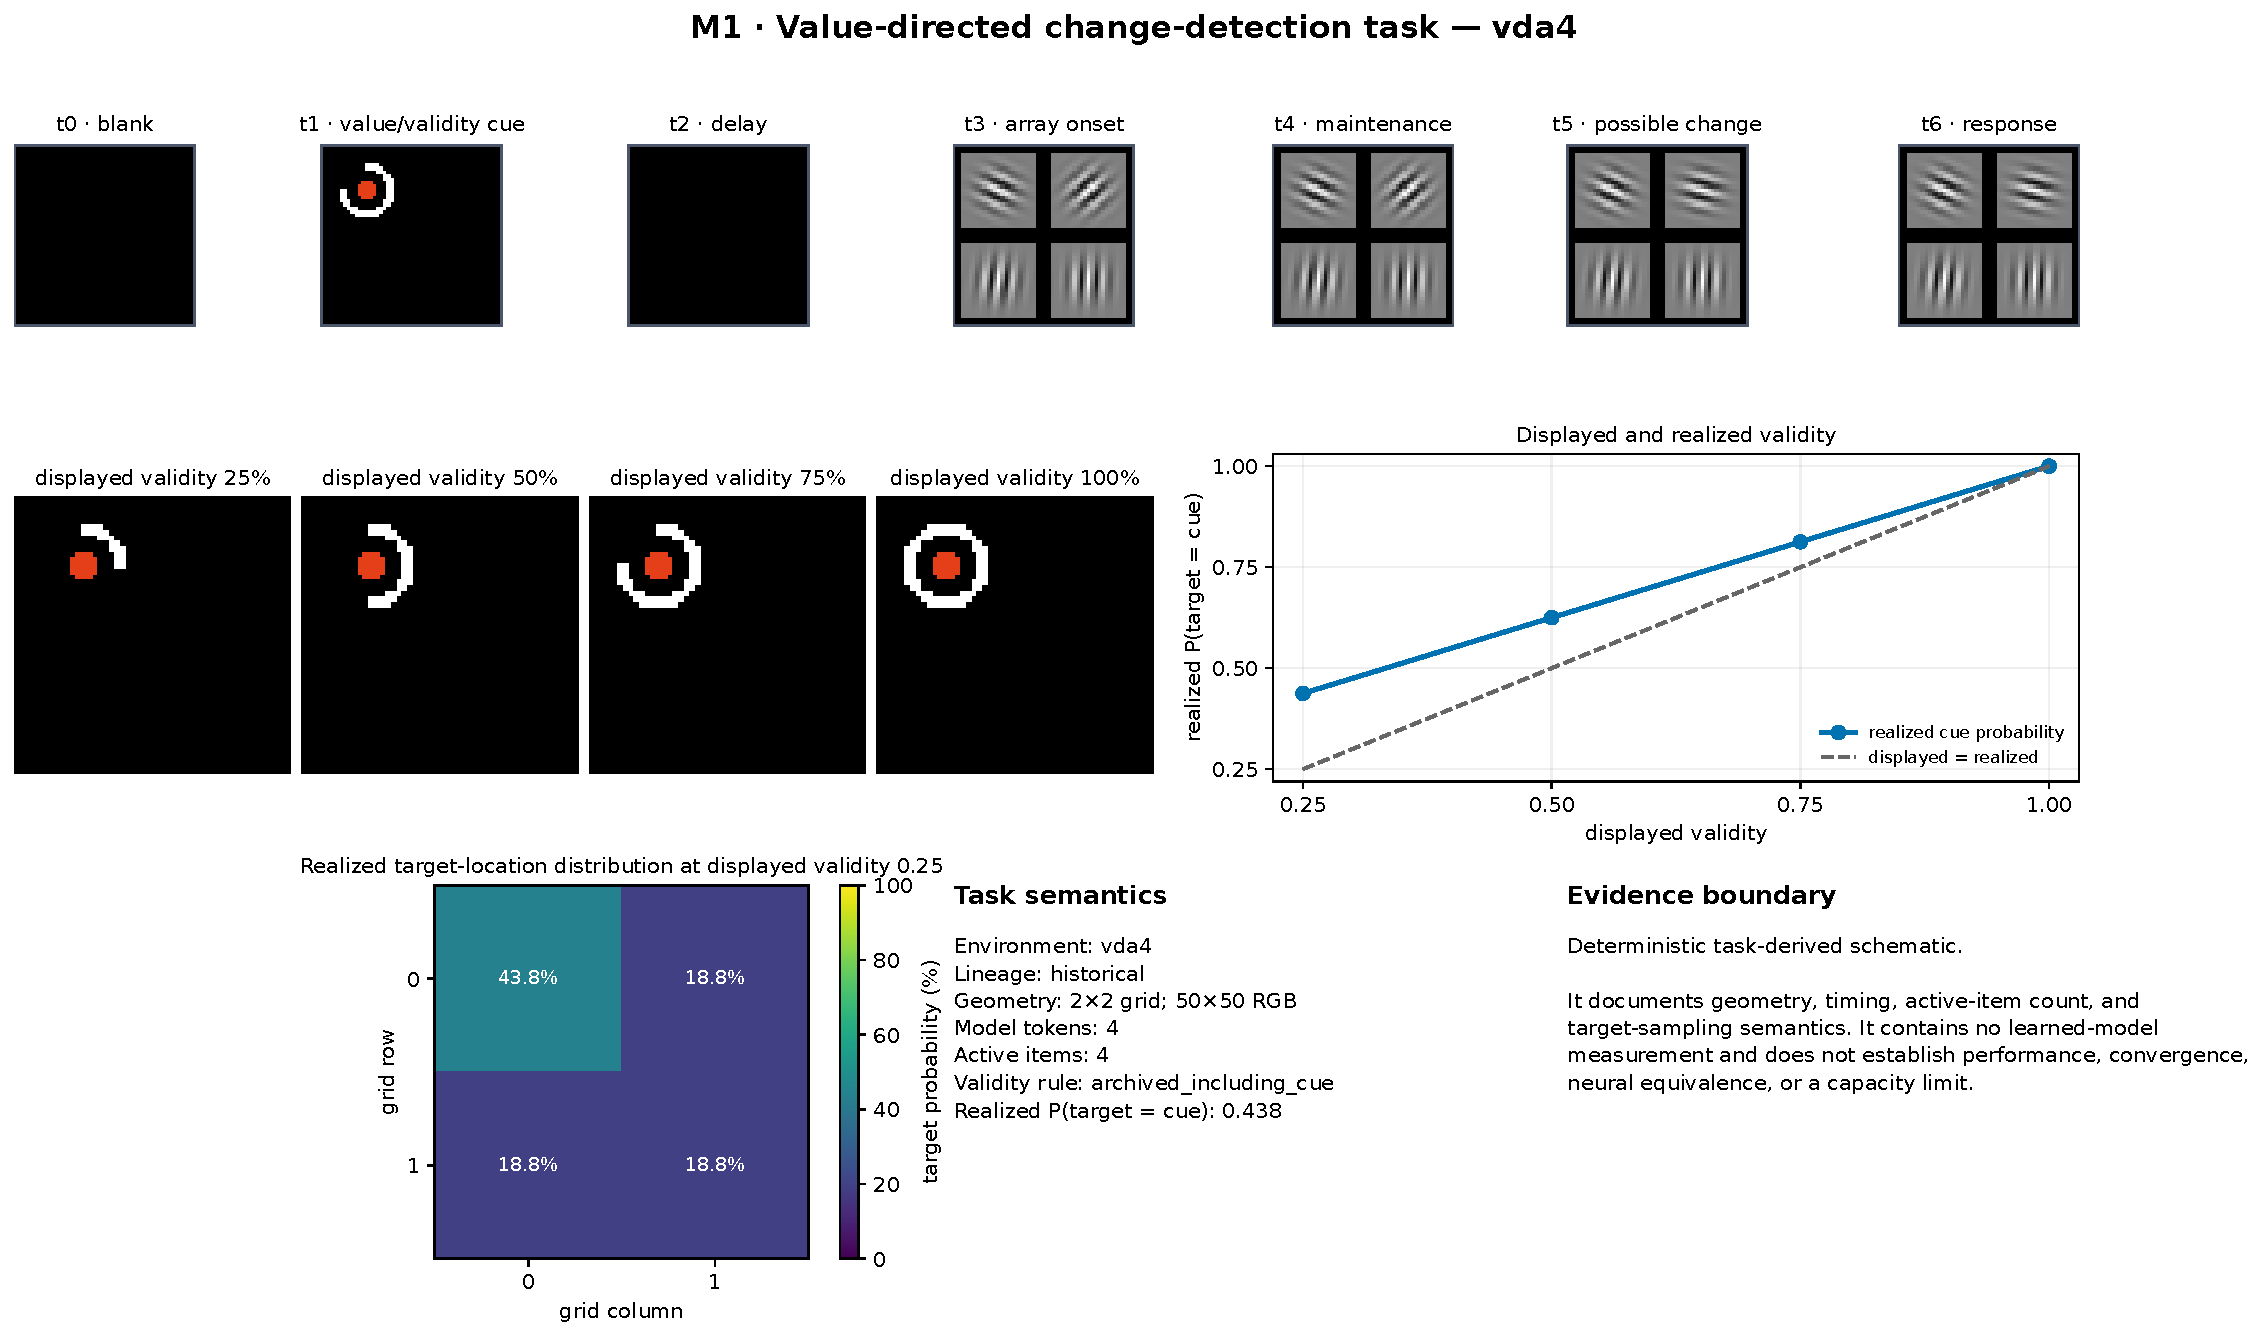
\includegraphics[width=0.97\linewidth]{m1_task_vda4.pdf}
\captionof{figure}{\textbf{Historical VDA4 task specification.} \eclass{Deterministic task-derived schematic.} The figure documents the seven-frame sequence, $2\times2$ geometry, four active items, four model tokens, and archived cue-including validity. At displayed validity 0.25, the realized cue probability is 0.438.}\label{fig:m1-historical}
\end{center}
\end{landscape}

\begin{landscape}
\thispagestyle{plain}
\begin{center}
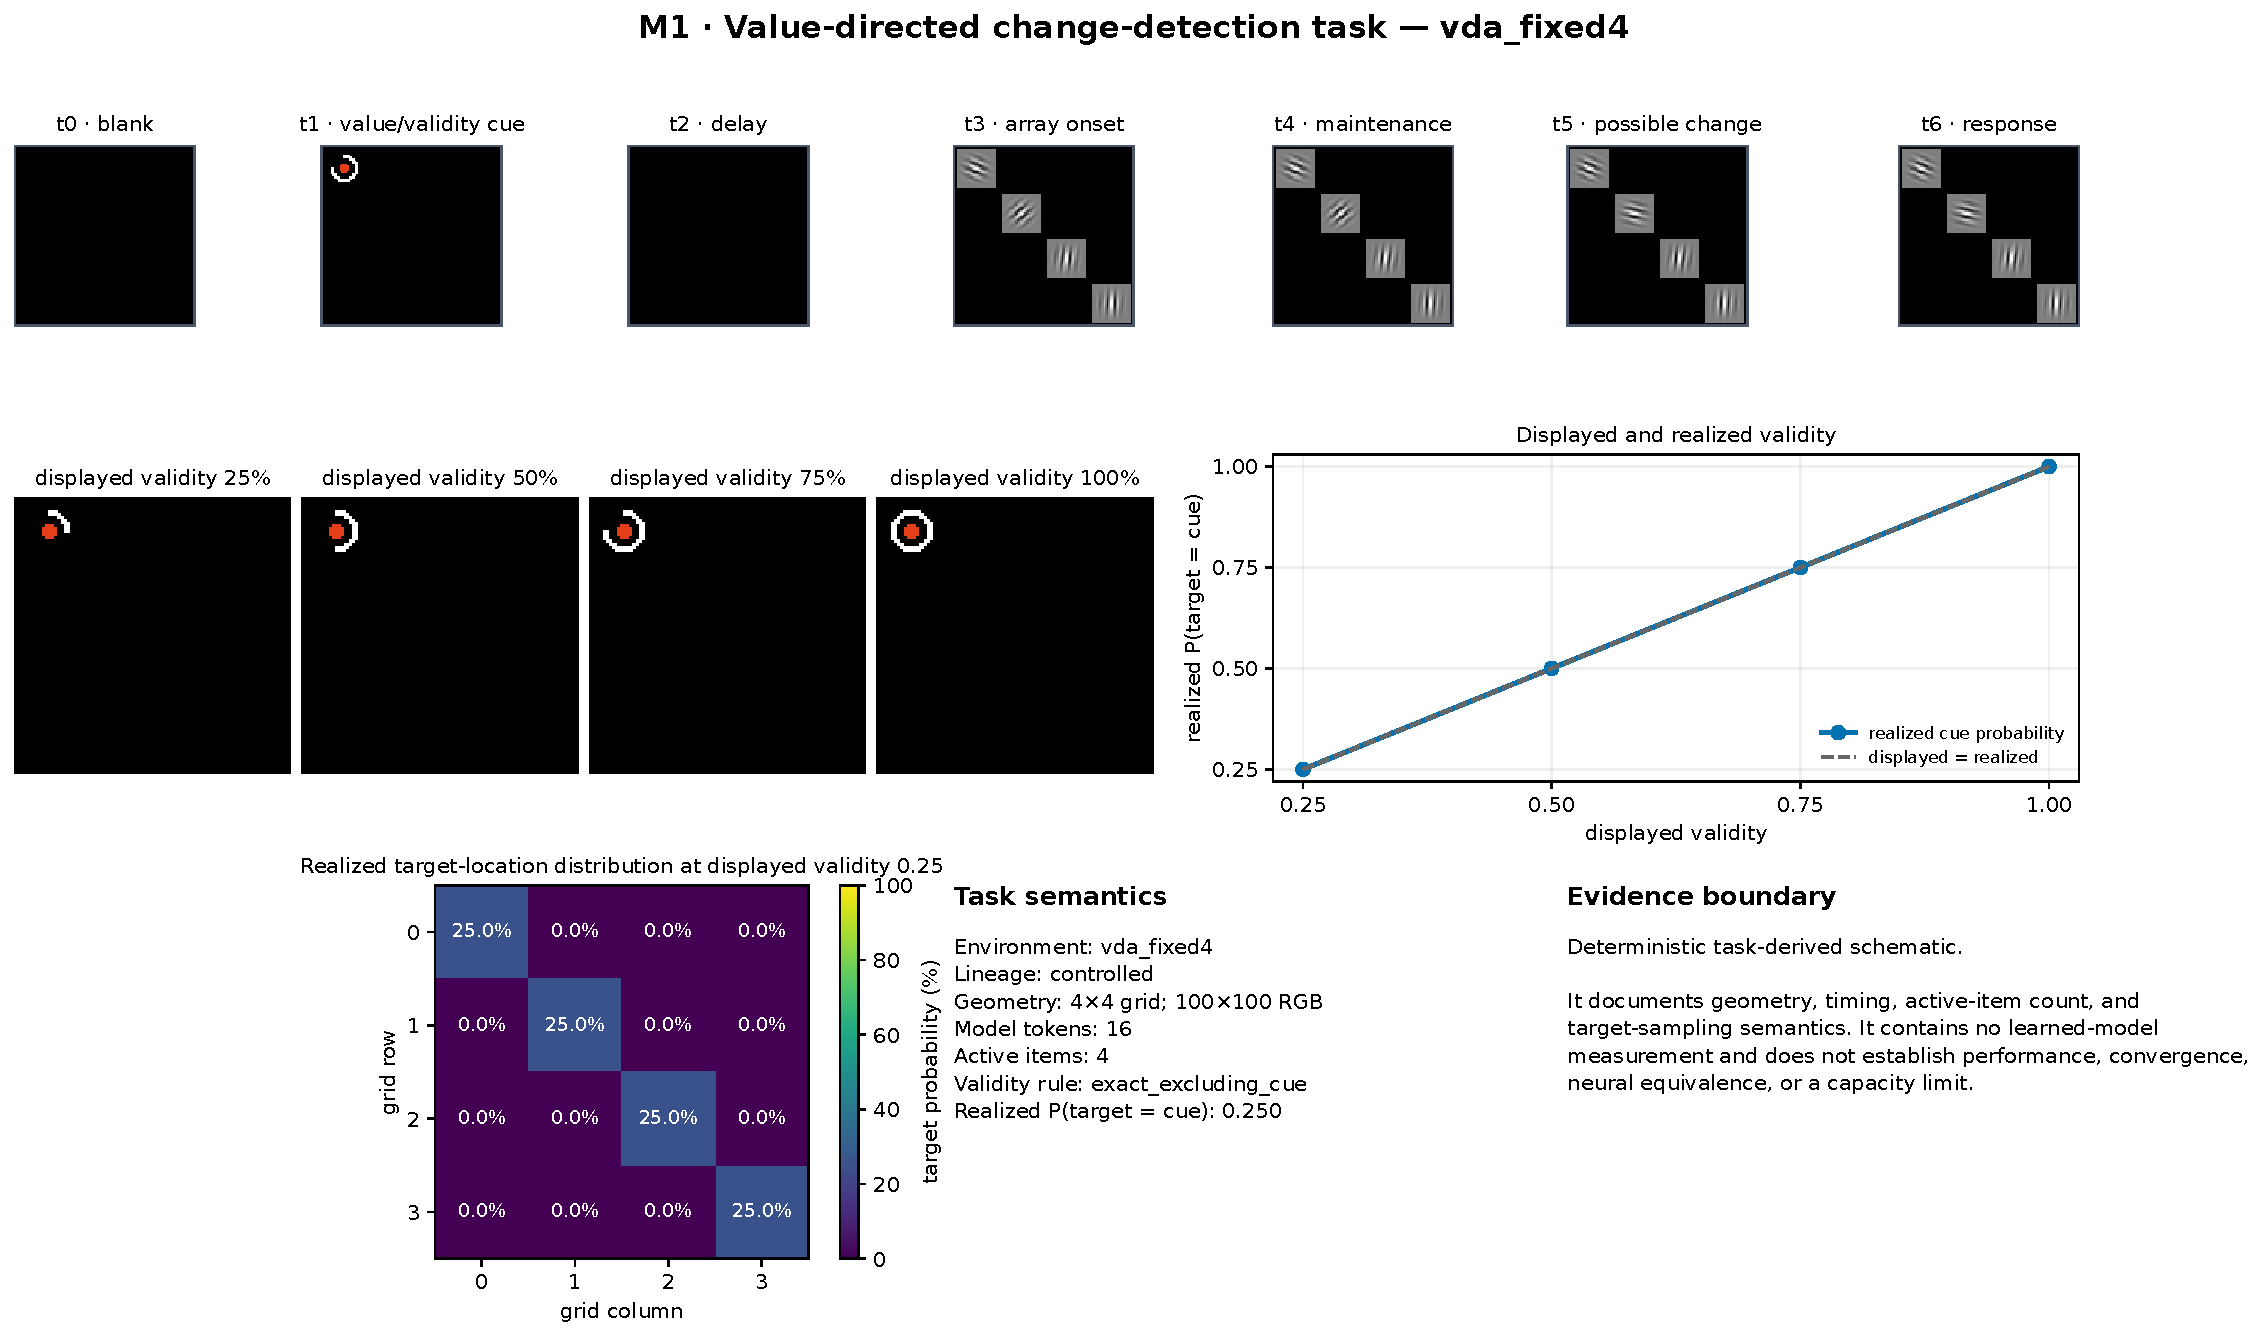
\includegraphics[width=0.97\linewidth]{m1_task_vda_fixed4.pdf}
\captionof{figure}{\textbf{Controlled fixed-grid VDA4 task specification.} \eclass{Deterministic task-derived schematic.} Across the controlled fixed-grid series, geometry is held at $4\times4$; unlike historical VDA4, this four-active-item task therefore has sixteen model tokens. Invalid targets exclude the cue, making displayed and realized validity equal.}\label{fig:m1-controlled}
\end{center}
\end{landscape}

\subsection{Recurrent architecture}\label{sec:architecture}
The architecture figures were generated from source-hashed specifications of \path{model.py}, \path{paper_encoder.py}, \path{paper_heads.py}, and \path{conv_frontend.py}. The shared pipeline preserves patch structure through routing and recurrent memory, then removes it at the actor/critic readout (Figure~\ref{fig:m2a}). In \env{affine\_ew}, memory produces element-wise scale and shift terms before self-attention (Figure~\ref{fig:m2b}). The spatial xLSTM updates a recurrent state independently at each patch position with shared parameters and feeds the next routing step (Figure~\ref{fig:m2c}). The \env{crossattn1} comparator instead queries with current visual tokens and concatenates visual and memory keys and values (Figure~\ref{fig:m2d}).

\captionof{table}{\textbf{Source-grounded architecture components.} Each row identifies the current-source anchor and the computational property audited from it.}\label{tab:architecture-components}
\begin{tabularx}{\textwidth}{@{}p{2.8cm}p{4.2cm}Y@{}}
\toprule
Component & Source anchor & Audited property\\
\midrule
Visual stem & \path{conv_frontend.py} & Converts the current RGB frame to a spatial token sequence; token count follows task geometry.\\
Affine router & \path{paper_encoder.py} & Applies memory-conditioned element-wise scale and shift before self-attention.\\
Cross-attention router & \path{paper_encoder.py} & Uses visual queries with visual and recurrent-memory keys and values.\\
Spatial recurrent state & \path{paper_encoder.py} & Updates xLSTM hidden and cell states independently by patch position with shared weights.\\
Policy/value readout & \path{paper_heads.py} & Flattens recurrent patch state for the two-action actor and quantile-regression critic.\\
Auxiliary predictor & \path{model.py} & Can add a training-only JEPA objective when enabled with nonzero loss weight; it is not part of inference-time behavior.\\
\bottomrule
\end{tabularx}

Both routers, and the multiplicative and matrix-affine variants used only in the intervention battery (Section~\ref{sec:intervention}), expose the same additive key-logit hook: any attention score can be biased at any chosen spatial key before the softmax, independent of the input used to construct the trial. That hook is what makes the causal-intervention program in Section~\ref{sec:intervention} possible on this architecture in the first place -- there is exactly one token per active item, so the attention map is a legible $N$-way array rather than a hundred-way patch grid, and a bias can be pointed at a single named location (the cue, the true change site, or an uninvolved control site) rather than at an anonymous patch.

\begin{landscape}\thispagestyle{plain}\begin{center}
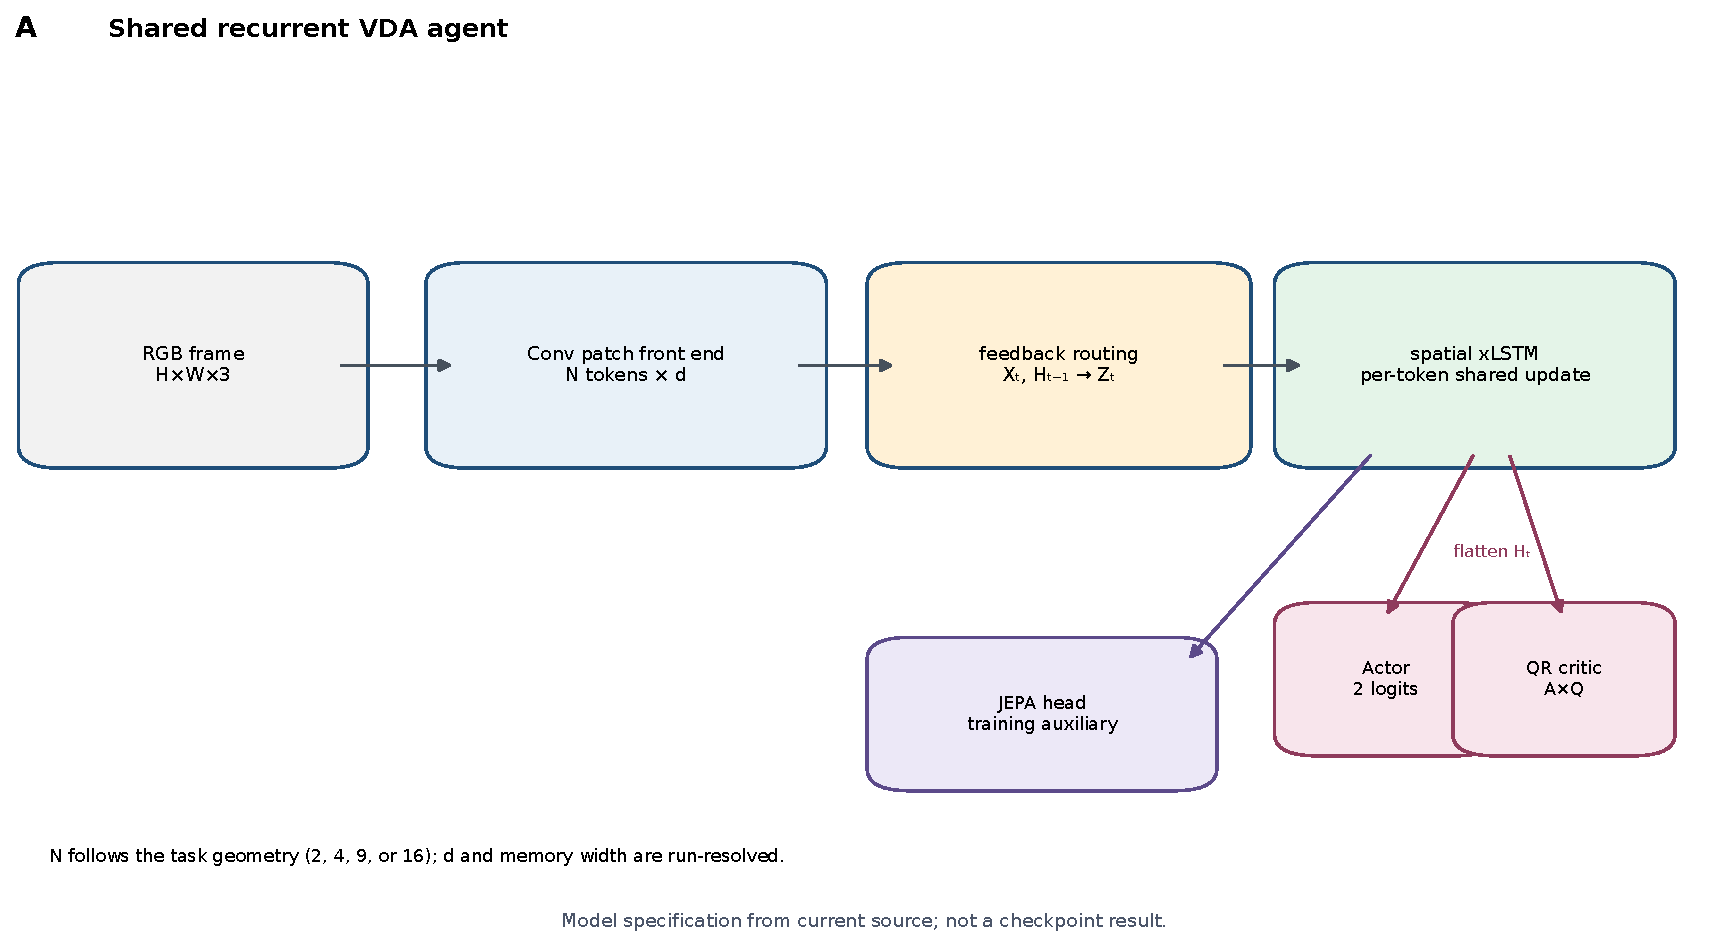
\includegraphics[width=0.97\linewidth]{m2_architecture_a.pdf}
\captionof{figure}{\textbf{M2A: shared recurrent agent.} \eclass{Source-derived model specification.} RGB frames become spatial patch tokens, undergo feedback routing, update a shared spatial xLSTM, and feed actor, quantile-regression critic, and an optional training-only JEPA readout.}\label{fig:m2a}
\end{center}\end{landscape}

\begin{landscape}\thispagestyle{plain}\begin{center}
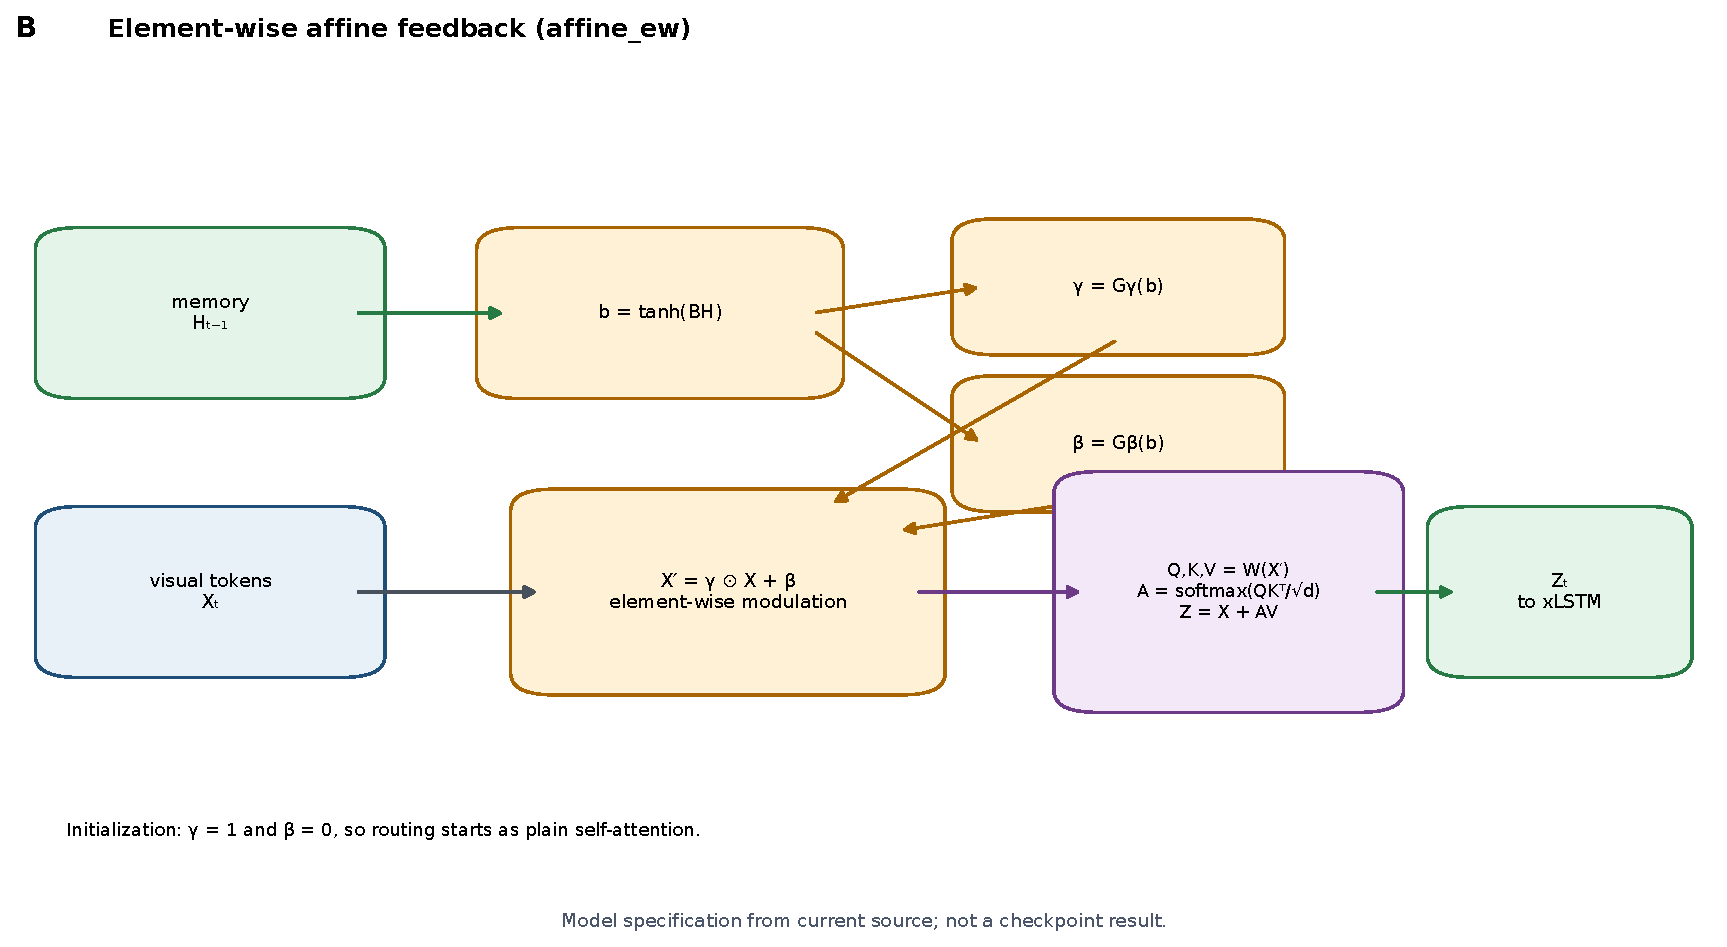
\includegraphics[width=0.97\linewidth]{m2_architecture_b.pdf}
\captionof{figure}{\textbf{M2B: element-wise affine feedback.} \eclass{Source-derived model specification.} Previous memory generates scale $\gamma$ and shift $\beta$, producing $X'=\gamma\odot X+\beta$ before self-attention. Identity initialization starts with $\gamma=1$ and $\beta=0$.}\label{fig:m2b}
\end{center}\end{landscape}

\begin{landscape}\thispagestyle{plain}\begin{center}
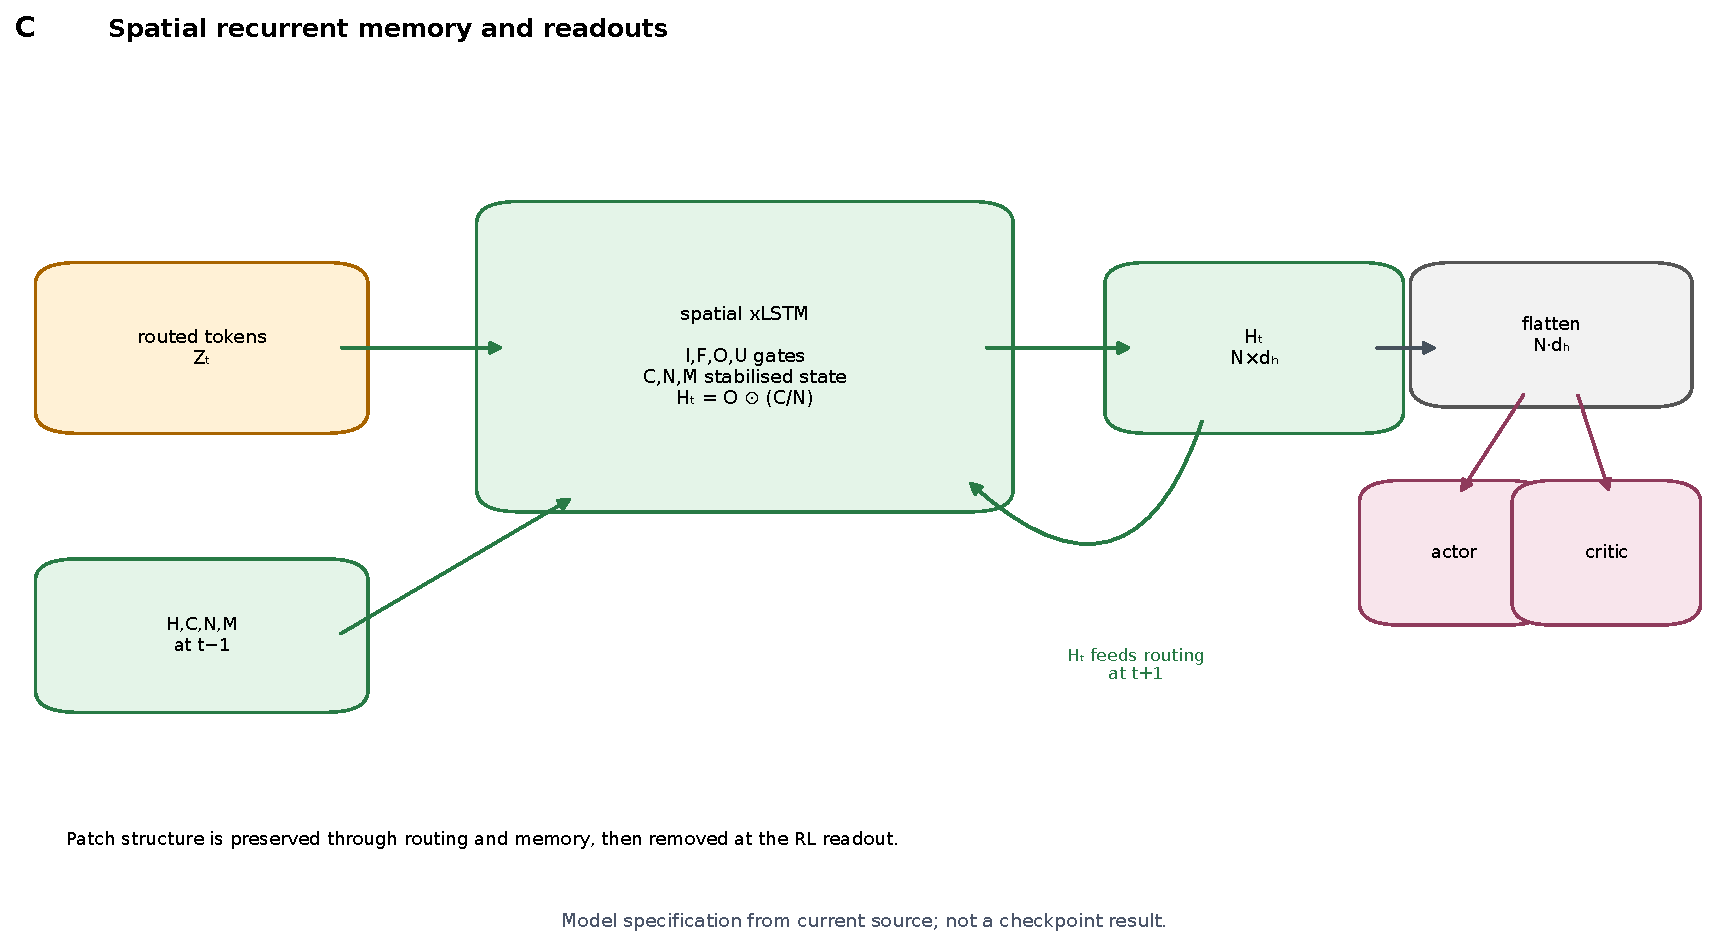
\includegraphics[width=0.97\linewidth]{m2_architecture_c.pdf}
\captionof{figure}{\textbf{M2C: spatial recurrent memory and readouts.} \eclass{Source-derived model specification.} Routed tokens and prior recurrent states enter the spatial xLSTM; the new hidden state both supplies the next routing step and, after flattening, feeds actor and critic.}\label{fig:m2c}
\end{center}\end{landscape}

\begin{landscape}\thispagestyle{plain}\begin{center}
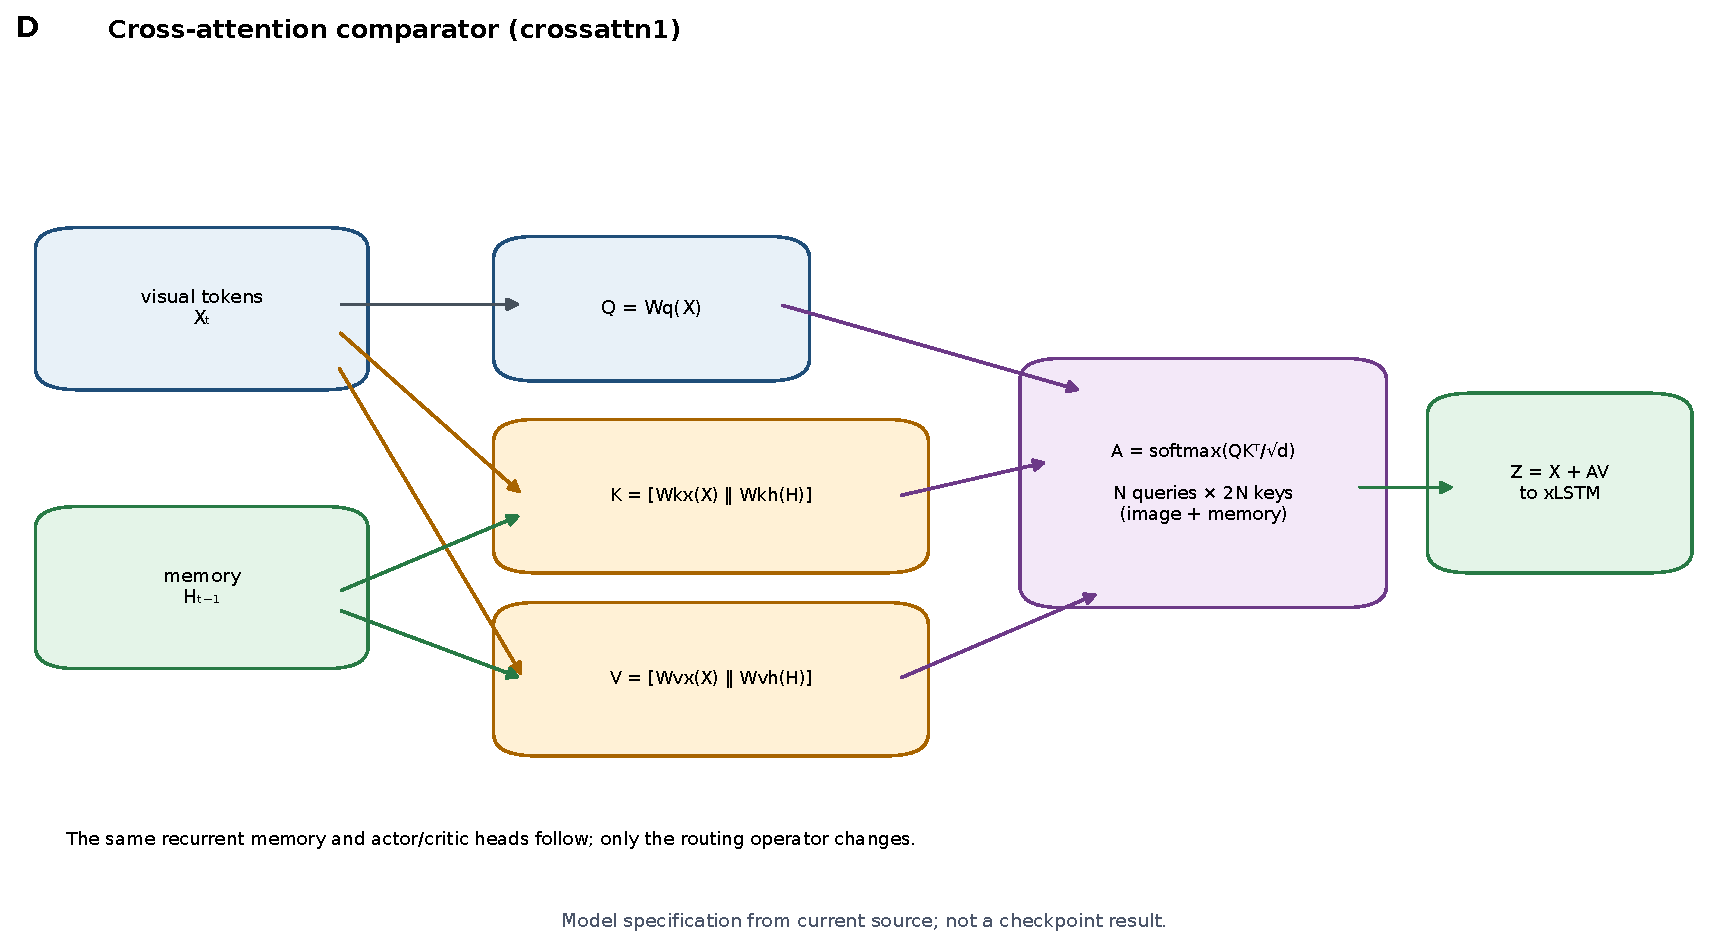
\includegraphics[width=0.97\linewidth]{m2_architecture_d.pdf}
\captionof{figure}{\textbf{M2D: cross-attention comparator.} \eclass{Source-derived model specification.} Current visual tokens provide queries while visual and recurrent-memory streams jointly provide keys and values. The same recurrent memory and policy heads follow; only the routing operator changes.}\label{fig:m2d}
\end{center}\end{landscape}

\section{Behavioral signatures: psychometric and chronometric functions, cueing effects}\label{sec:behavior}
This section asks the question the field has always started with: does the model behave like a cued observer, and how large is that benefit? We build the argument from the broadest, lowest-evidence-tier data to the narrowest, most rigorously controlled data, because the pattern is consistent across that whole range and the strength of the claim should track the strength of the evidence. Sensitivity and criterion are addressed together with response probability wherever the underlying signal-detection decomposition is available, following Carrasco's separation of discriminability from response bias and Luo and Maunsell's demonstration that a more liberal declaration policy can raise hit rate without improving sensory evidence \cite{carrasco2011,luo2018}; where only response probability is available, we say so rather than calling it sensitivity.

\subsection{Historical set-size series: a broad but loosely controlled landscape}\label{sec:historical-behavior}
The admitted historical figures read only the preserved \path{vda_sweep/figs/psych.npz} cache, an aggregate archive with no producer hash, checkpoint hash, or per-point trial count; plotting does not import Torch or execute a checkpoint. Each figure displays change-response probability and conditional mean response frame over ten orientation-change magnitudes and four displayed validity levels. Across included entries, larger orientation changes are generally associated with higher change-response probability and a lower conditional mean response frame, and some VDA4 and VDA9 entries show descriptive cued-vs-uncued separation (Figure~\ref{fig:m3-overview}; full-resolution plates in Appendix~\ref{app:m3-full}). VDA1 has only one active item, so an uncued comparator is undefined (Figure~\ref{fig:m3-overview}, and Appendix~\ref{app:m3-full} Figures~\ref{fig:m3-vda1-affine}--\ref{fig:m3-vda1-cross}); in VDA2 the cued and archived-uncued curves are close in several panels, which is a descriptive property of these cache entries rather than a precision-tested null. Because these are separately trained checkpoints represented as aggregate point estimates with no reconstructable interval, this series establishes a qualitative landscape -- cueing looks behaviorally real across the historical ladder -- and nothing quantitative beyond it.

\clearpage
\thispagestyle{plain}
\begin{center}
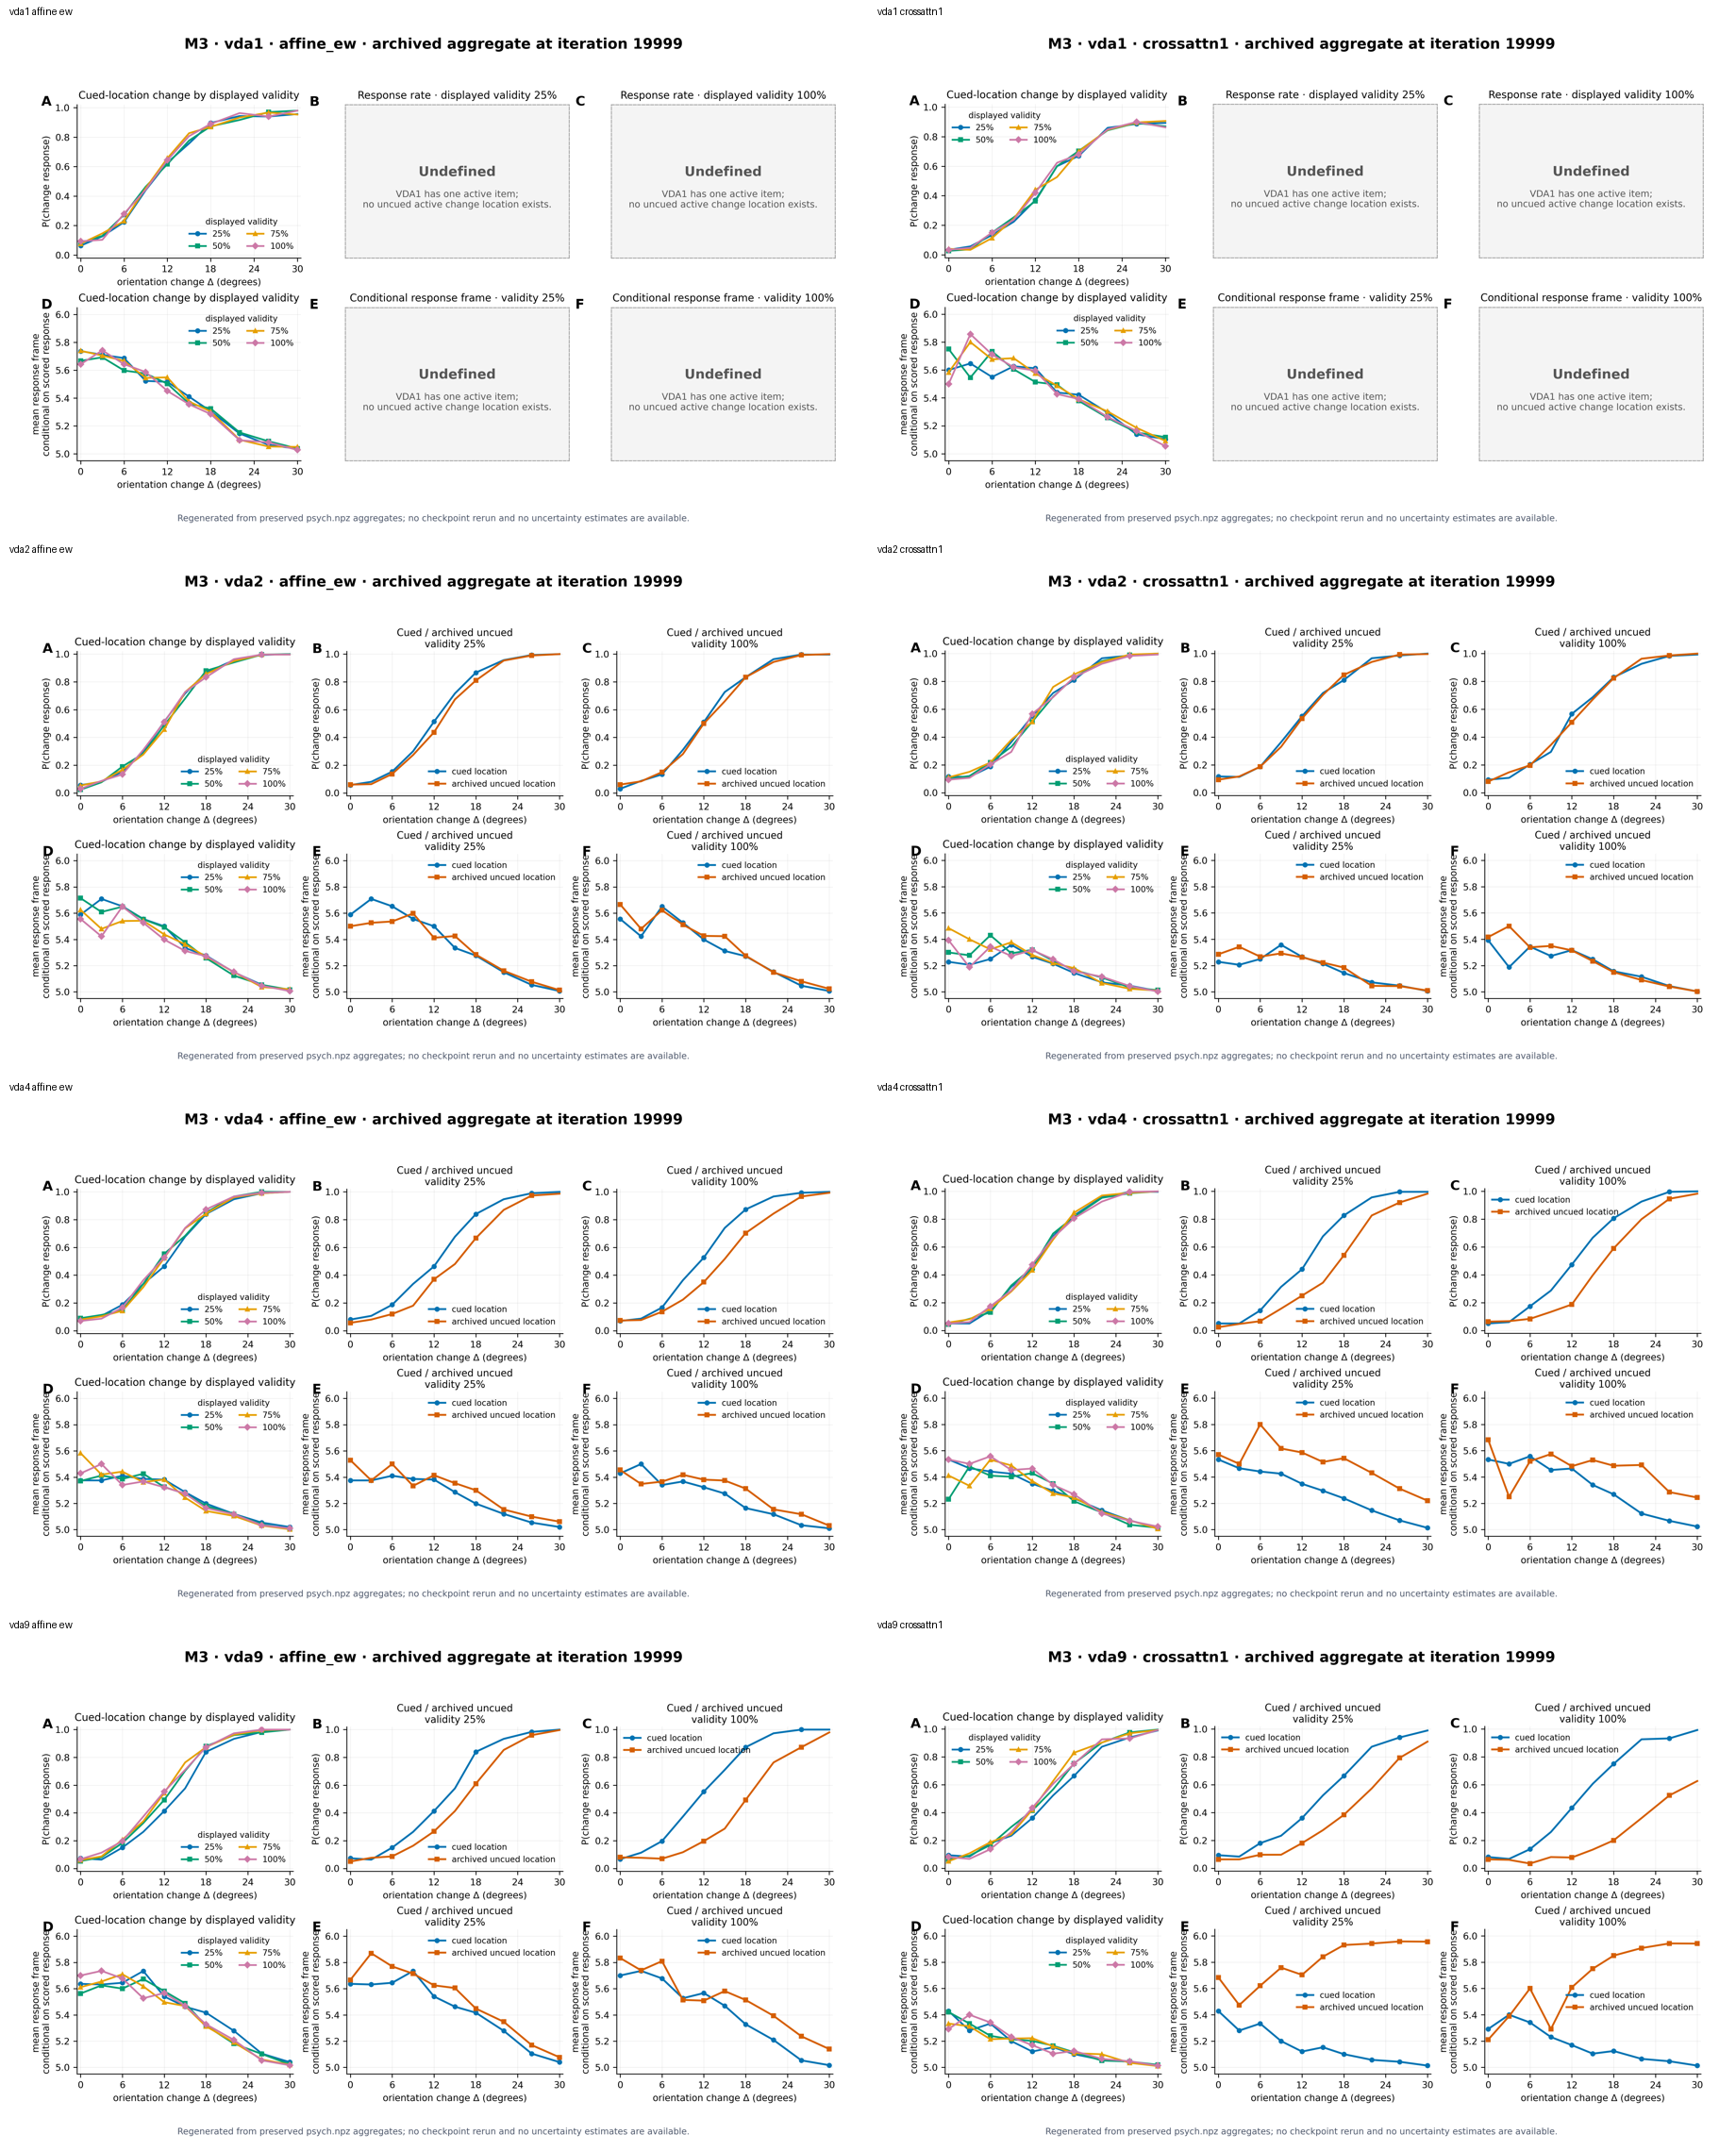
\includegraphics[width=0.96\linewidth]{m3_behavior_contact_sheet.png}
\captionof{figure}{\textbf{Comparative historical behavior overview.} \eclass{Regenerated from preserved aggregate NPZ; checkpoints not rerun.} Rows descend through VDA1, VDA2, VDA4, and VDA9; columns show affine then cross-attention routing. Panels A--C show response probability and D--F conditional mean response frame; color encodes displayed validity in cued panels and spatial condition in cued-vs-archived-uncued panels. VDA1 uncued estimands are undefined; VDA2 cued and archived-uncued curves are often close without establishing a precise null; some VDA4/VDA9 entries show descriptive separation. Appendix~\ref{app:m3-full} contains the eight full-resolution plates.}\label{fig:m3-overview}
\end{center}
\clearpage

\subsection{Checkpoint-verified psychometrics: VDA4 and VDA9}\label{sec:first-wave-behavior}
The first wave is a separate, provenance-closed recomputation from one independently selected iteration-19{,}999 checkpoint for each task--routing label (historical VDA4 and VDA9 crossed with \env{affine\_ew} and \env{crossattn1}), with an immutable 77-file production tree binding executable source, dependencies, checkpoints, runtime, and deterministic caches (manifest SHA-256 \texttt{c58a864a\ldots8c45706}). All first-wave protocols fix the red cue at S1; the bottom-right invalid comparator is S4 for VDA4 and S9 for VDA9 (Figures~\ref{fig:first-wave-env-vda4}--\ref{fig:first-wave-env-vda9}).

\begin{landscape}\thispagestyle{plain}\begin{center}
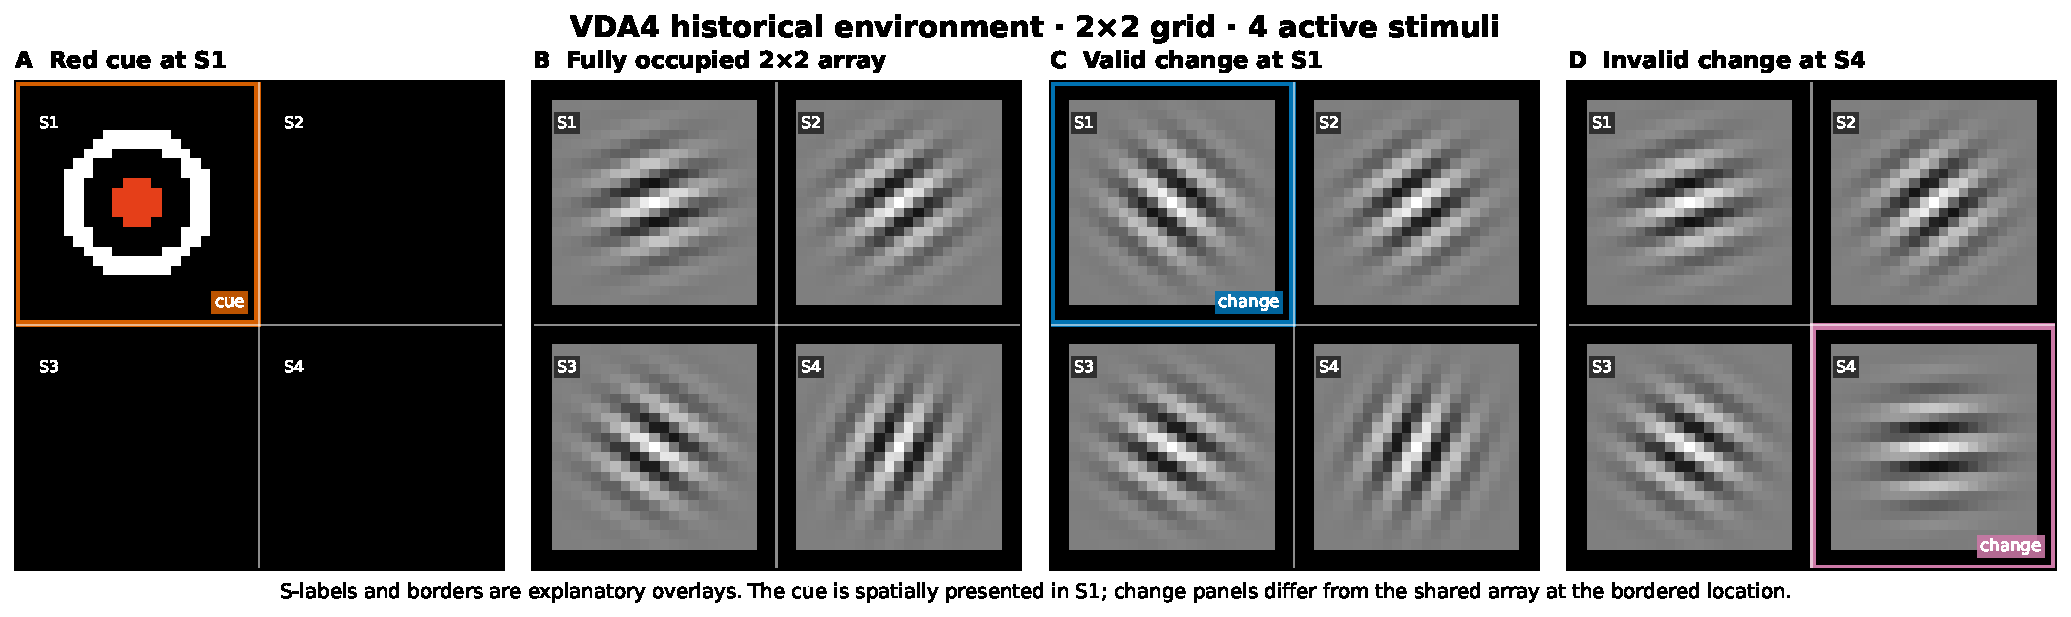
\includegraphics[width=0.90\linewidth]{first_wave_environment_vda4.pdf}
\captionof{figure}{\textbf{Verified historical VDA4 condition.} \eclass{Deterministic first-wave environment product.} The four occupied positions form the historical $2\times2$ geometry. S1 receives the red cue and the valid change; S4 is the registered bottom-right invalid location.}\label{fig:first-wave-env-vda4}
\vspace{0.6em}
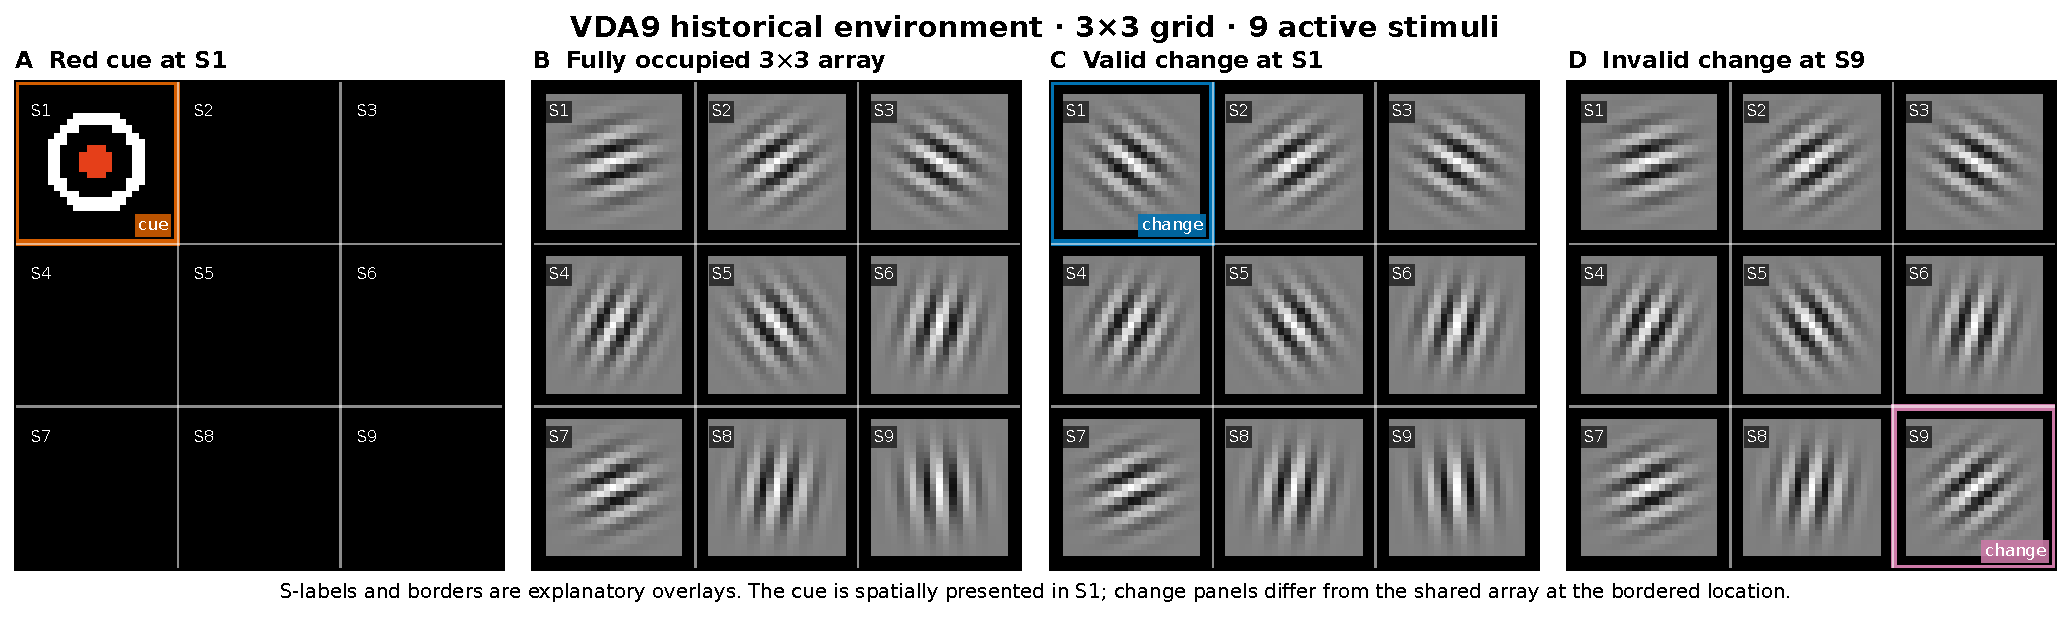
\includegraphics[width=0.90\linewidth]{first_wave_environment_vda9.pdf}
\captionof{figure}{\textbf{Verified historical VDA9 condition.} \eclass{Deterministic first-wave environment product.} The nine occupied positions form the historical $3\times3$ geometry. S1 receives the red cue and the valid change; S9 is the true bottom-right invalid location.}\label{fig:first-wave-env-vda9}
\end{center}\end{landscape}

Each psychometric point uses 300 evaluation trials; the ordinate is the probability of a qualifying change response (first declaration at logical frame 5 or later, divided by all 300 trials). Panels A and B fix the change at S1 or the bottom-right location, respectively, while sweeping displayed cue proportion; Panel C re-plots the 100\%-displayed endpoints of A and B as a within-checkpoint fixed-location contrast. Wilson 95\% intervals describe finite evaluation-trial uncertainty for one checkpoint, not training-seed variation. Change-response probability generally rises with orientation change, and fixed-S1 estimates generally exceed fixed-bottom-right estimates at intermediate magnitudes (Figures~\ref{fig:first-wave-psych-vda4-affine}--\ref{fig:first-wave-psych-vda9-cross}).

\begin{landscape}\thispagestyle{plain}\begin{center}
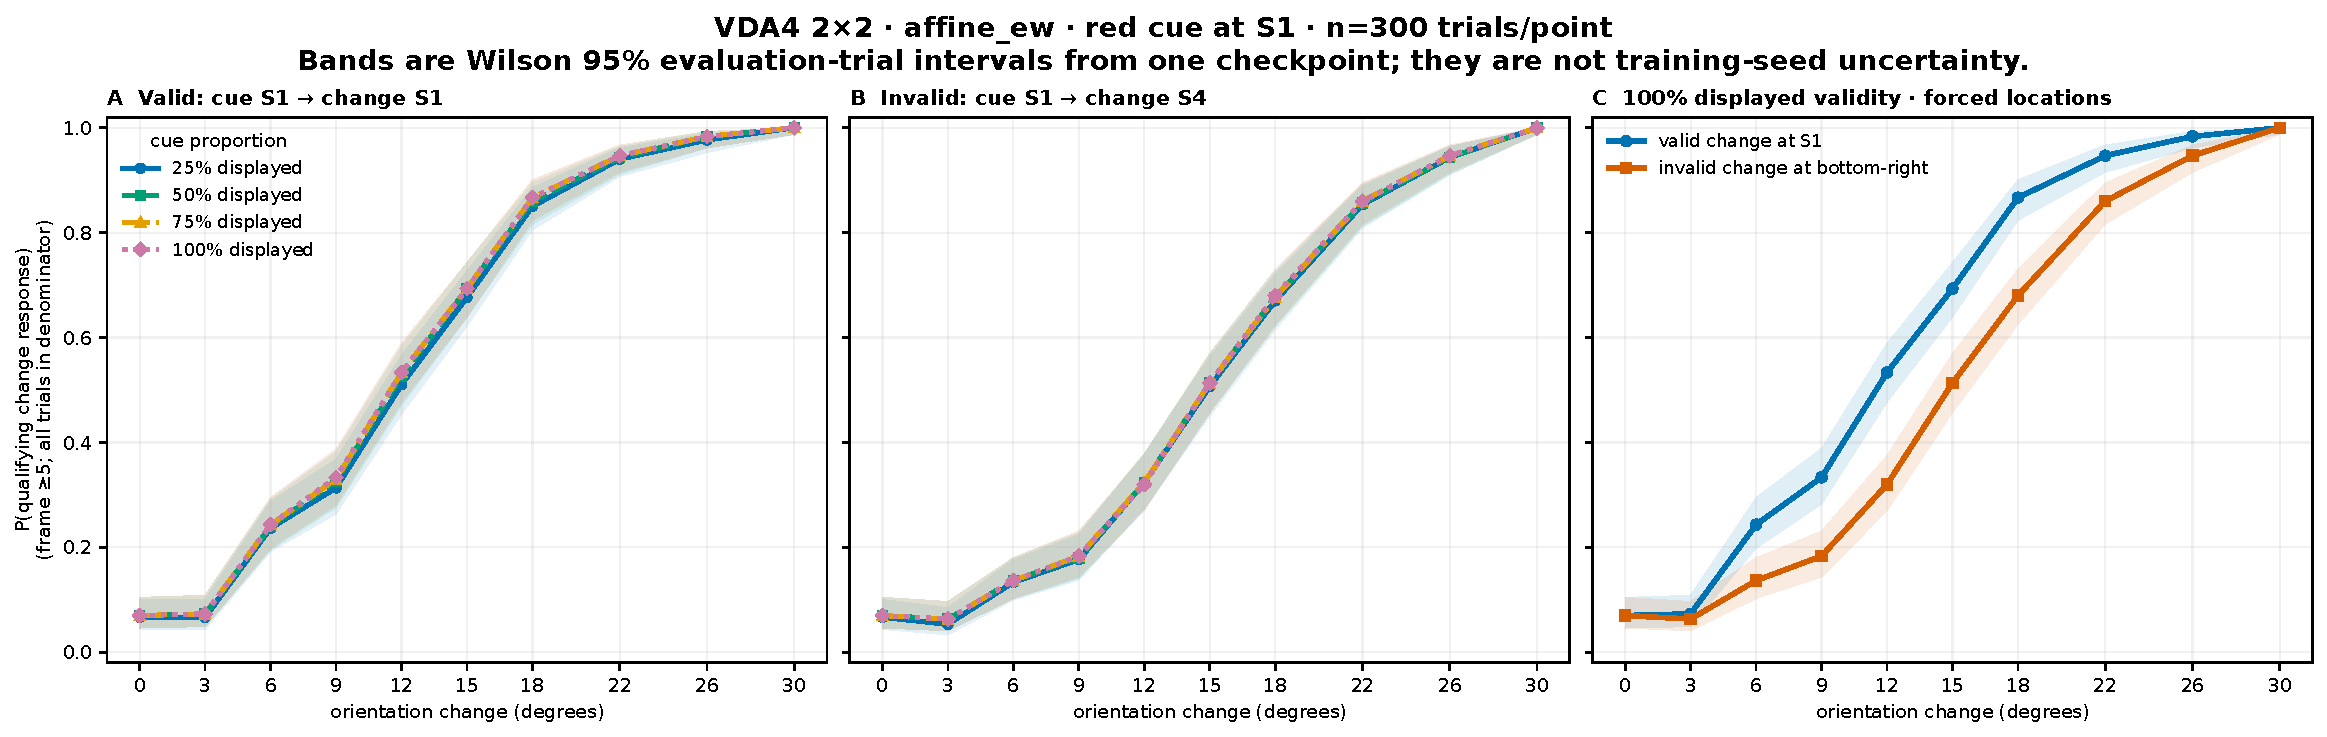
\includegraphics[width=0.84\linewidth]{first_wave_psychometric_vda4_affine_ew.pdf}
\captionof{figure}{\textbf{VDA4 affine psychometrics.} \eclass{Checkpoint-recomputed evaluation; 300 trials per point.} Panels A and B fix the change at S1 and S4, respectively, while sweeping displayed cue proportion. Panel C re-plots their 100\%-displayed endpoints. Bands are Wilson evaluation-trial intervals for one checkpoint.}\label{fig:first-wave-psych-vda4-affine}
\vspace{0.7em}
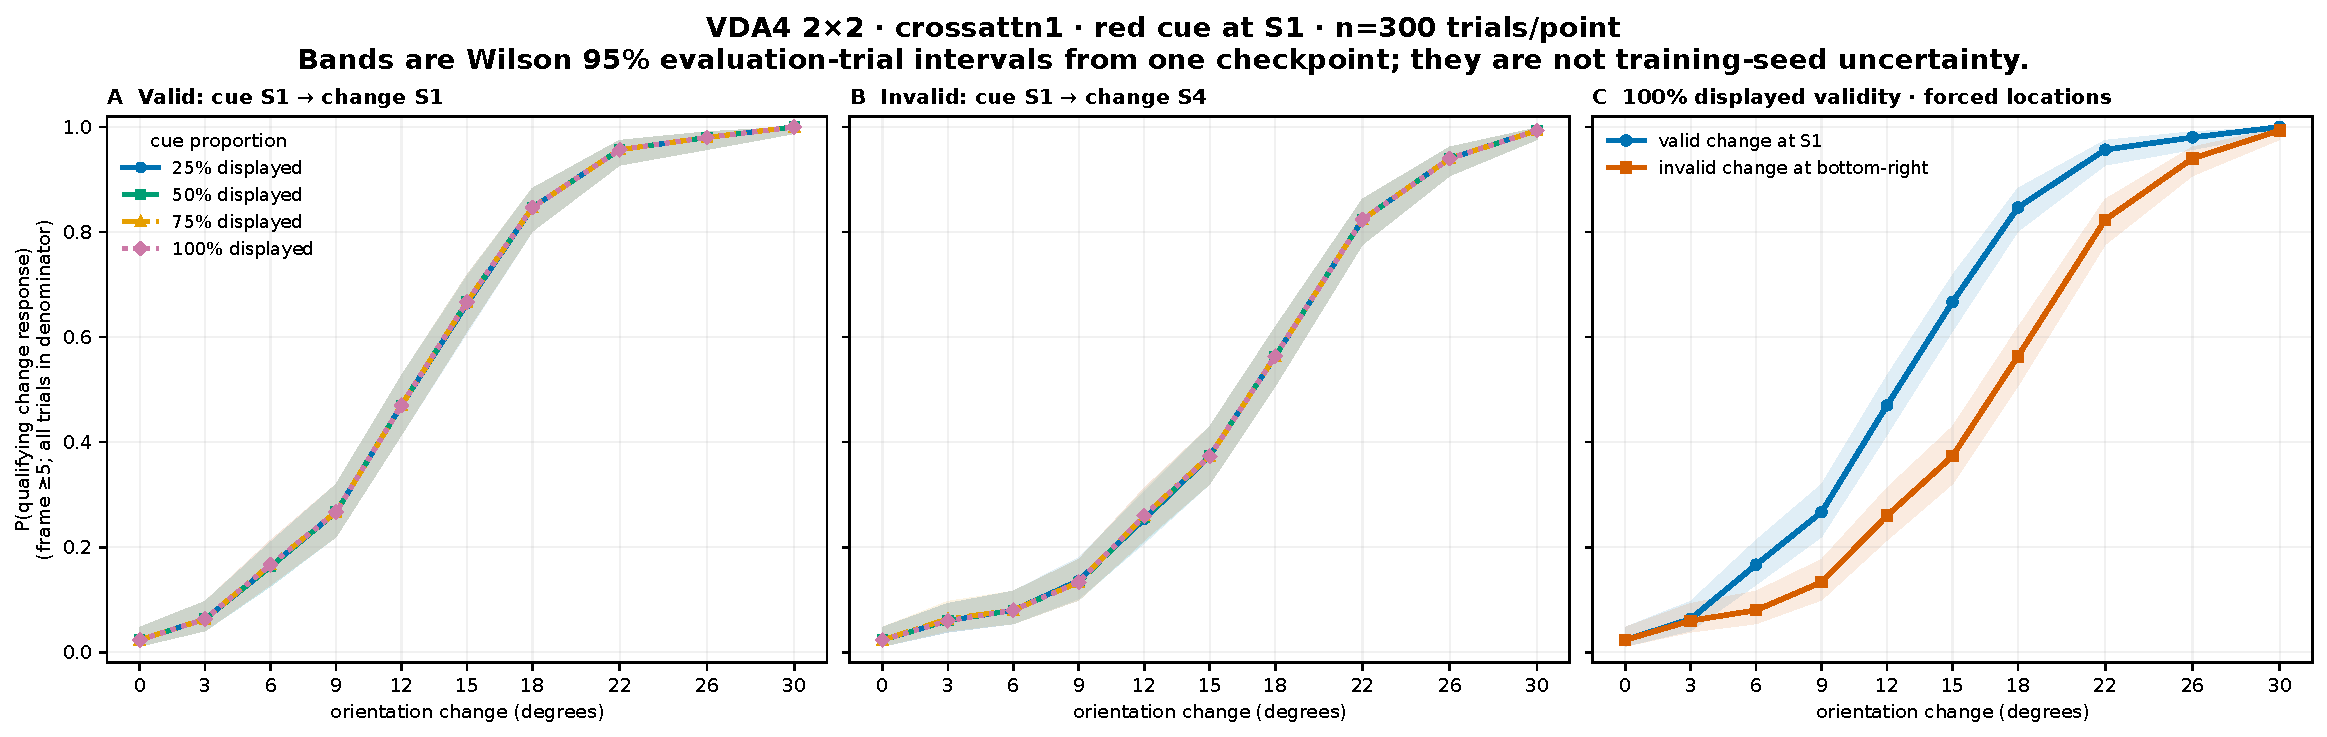
\includegraphics[width=0.84\linewidth]{first_wave_psychometric_vda4_crossattn1.pdf}
\captionof{figure}{\textbf{VDA4 cross-attention psychometrics.} \eclass{Checkpoint-recomputed evaluation; 300 trials per point.} Same protocol as Figure~\ref{fig:first-wave-psych-vda4-affine}. Separate checkpoints preclude a causal affine--cross-attention contrast.}\label{fig:first-wave-psych-vda4-cross}
\end{center}\end{landscape}

\begin{landscape}\thispagestyle{plain}\begin{center}
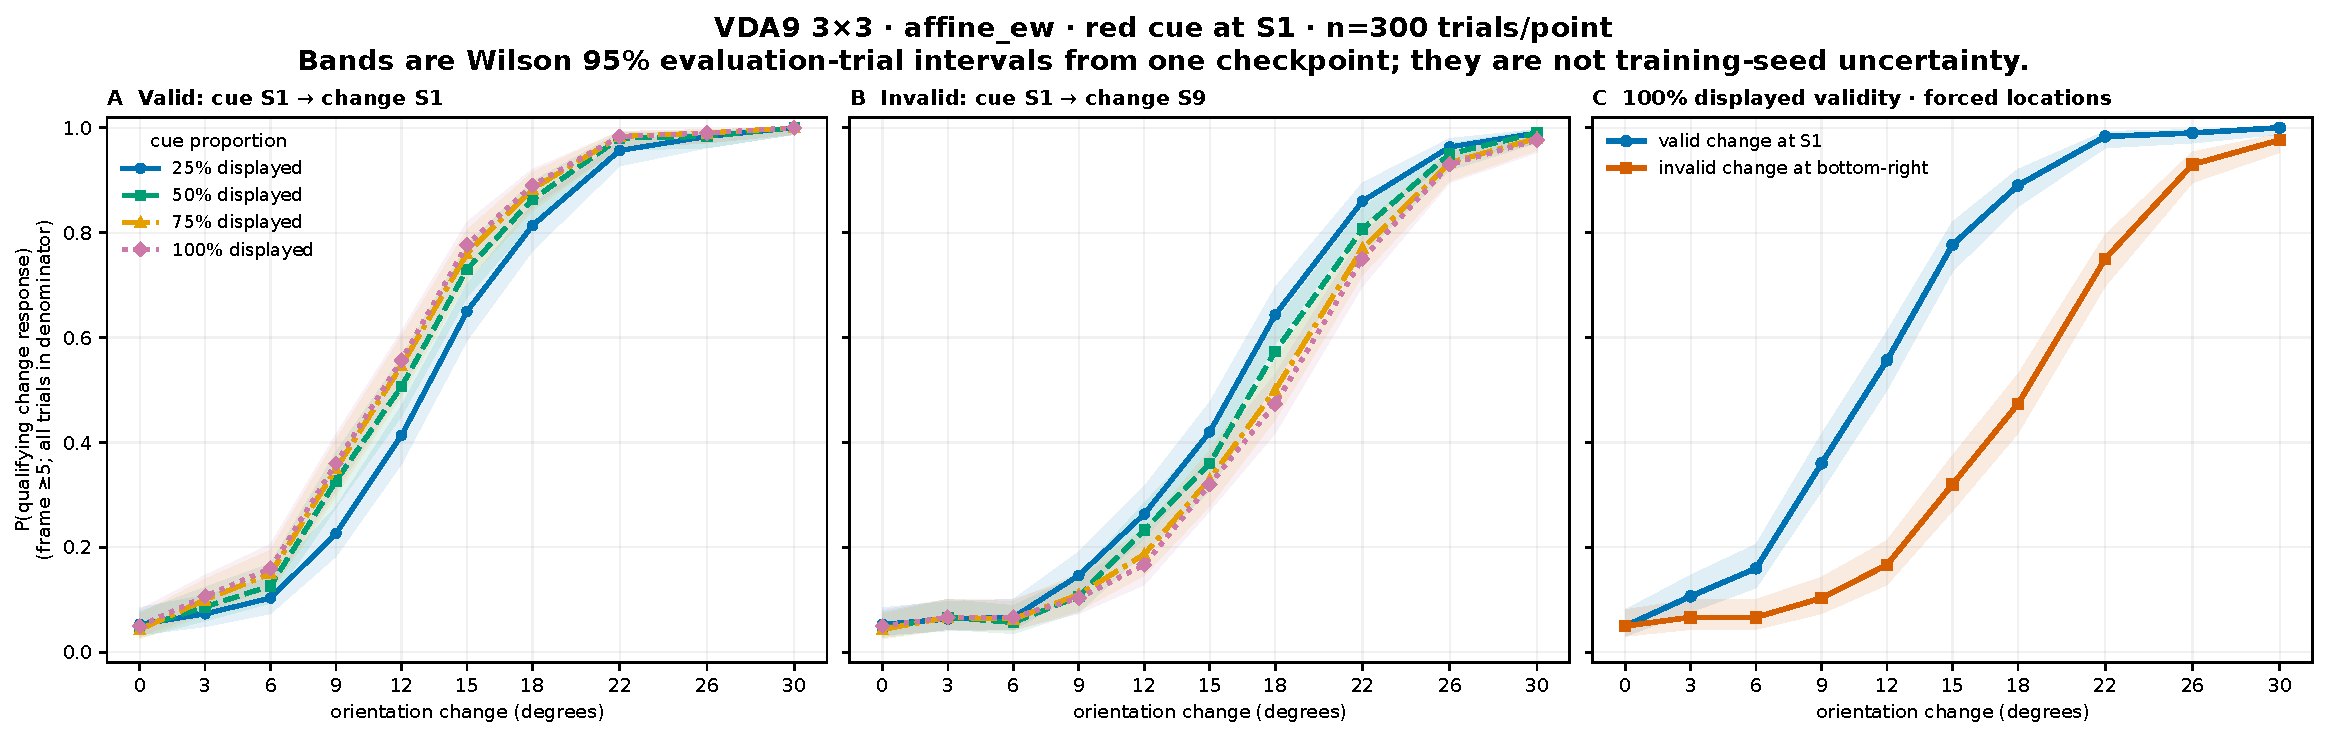
\includegraphics[width=0.80\linewidth]{first_wave_psychometric_vda9_affine_ew.pdf}
\captionof{figure}{\textbf{VDA9 affine psychometrics.} \eclass{Checkpoint-recomputed evaluation; 300 trials per point.} Panels A and B fix the change at S1 and S9, respectively; Panel C re-plots their 100\%-displayed endpoints. S9 is a specified bottom-right location, not a geometry-free ``opposing'' label.}\label{fig:first-wave-psych-vda9-affine}
\vspace{0.7em}
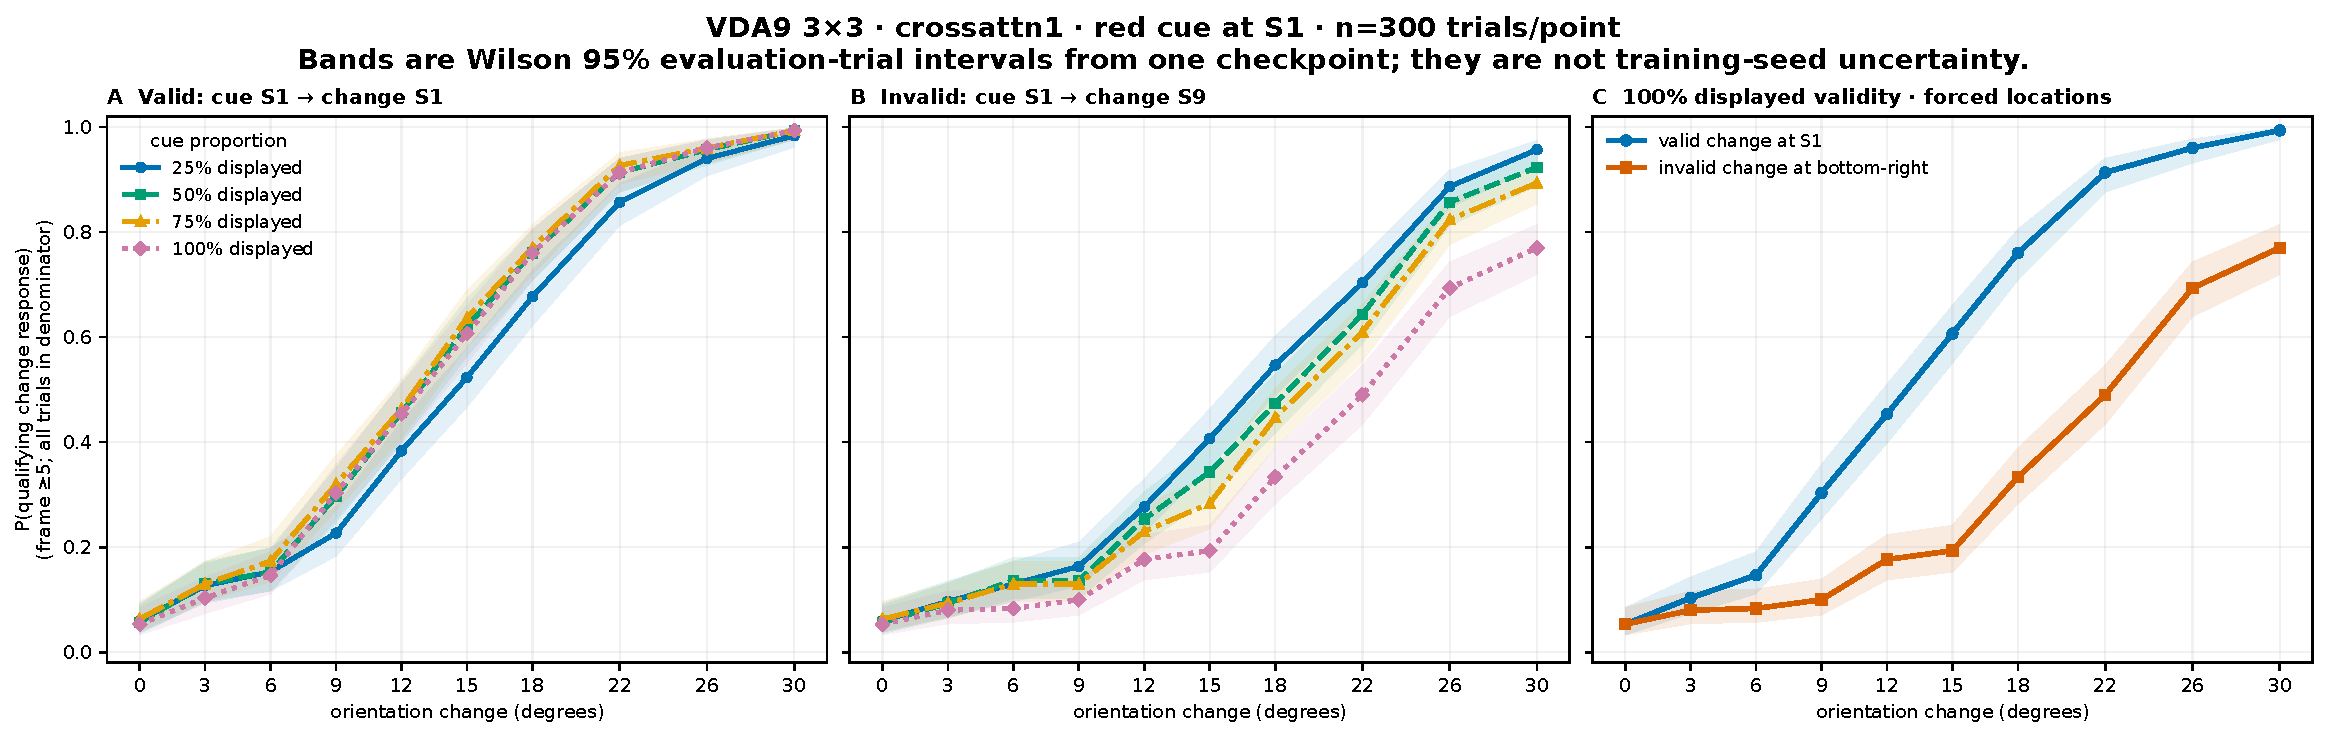
\includegraphics[width=0.80\linewidth]{first_wave_psychometric_vda9_crossattn1.pdf}
\captionof{figure}{\textbf{VDA9 cross-attention psychometrics.} \eclass{Checkpoint-recomputed evaluation; 300 trials per point.} The lower fixed-S9 response at large changes appears in both Panel B and its Panel C re-plot by construction, not replication.}\label{fig:first-wave-psych-vda9-cross}
\end{center}\end{landscape}

\subsection{Does recurrent width change the cueing benefit?}\label{sec:width-behavior}
A matched battery reuses the exact first-wave VDA4 and VDA9 checkpoints, adds VDA1, and pairs each with a separately trained checkpoint carrying twice the recurrent width ($d_\mathrm{mem}=256$ vs.\ 128; Table~\ref{tab:width-comparison}). Width is a descriptive grouping contrast here, not a causal manipulation: the paired checkpoints were trained separately, so a width difference is confounded with training-run variation. At $14^\circ$, the clearest opposing contrast is a 21-percentage-point increase for VDA1 cross-attention versus a 13-percentage-point decrease for VDA4 cross-attention when d256 is compared with d128 (300 forced-valid-location trials per point at displayed validity 0.75; Table~\ref{tab:absolute-behavior} gives every constituent curve behind Figure~\ref{fig:matched-width}A). The other three admitted pairs likewise do not share a common direction: \textbf{a wider recurrent state does not consistently produce a larger cueing benefit} in this battery. Two VDA2 pairs are blocked by a token-geometry mismatch and VDA9 cross-attention d256 fails the registered behavioral acceptance threshold, leaving five admitted pairs -- five checkpoint comparisons, not an independent-seed population.

\begingroup\small
\captionof{table}{\textbf{Configured d128/d256 checkpoint comparison.} Task geometry, routing family, sensory token width, and iteration are held fixed within each admitted pair; recurrent width, flattened readout dimension, parameter count, learned weights, and training trajectory are not all matched.}\label{tab:width-comparison}
\begin{tabularx}{\textwidth}{@{}p{4.0cm}Y Y Y@{}}
\toprule
Quantity & d128 checkpoint & d256 checkpoint & Pairwise status\\
\midrule
Per-location recurrent state & $H,C,N,M$: 128 coordinates & $H,C,N,M$: 256 coordinates & Configured difference\\
Flattened actor/critic input & 512 (four tokens) or 1152 (nine) & 1024 (four tokens) or 2304 (nine) & Consequence of \texttt{d\_mem}\\
Sensory token width & 140 (four-token tasks) or 145 (VDA9) & Same as d128 & Held fixed within pair\\
Trainable parameters & 2.200--2.545 million & 2.805--3.509 million & Task- and routing-dependent\\
Task geometry and tokens & VDA1/VDA4: four; VDA9: nine & Same as d128 & Held fixed within admitted pair\\
Checkpoint & Iteration 19999 & Iteration 19999 & Separately trained weights\\
\bottomrule
\end{tabularx}
\endgroup

\begin{landscape}\thispagestyle{plain}\begin{center}
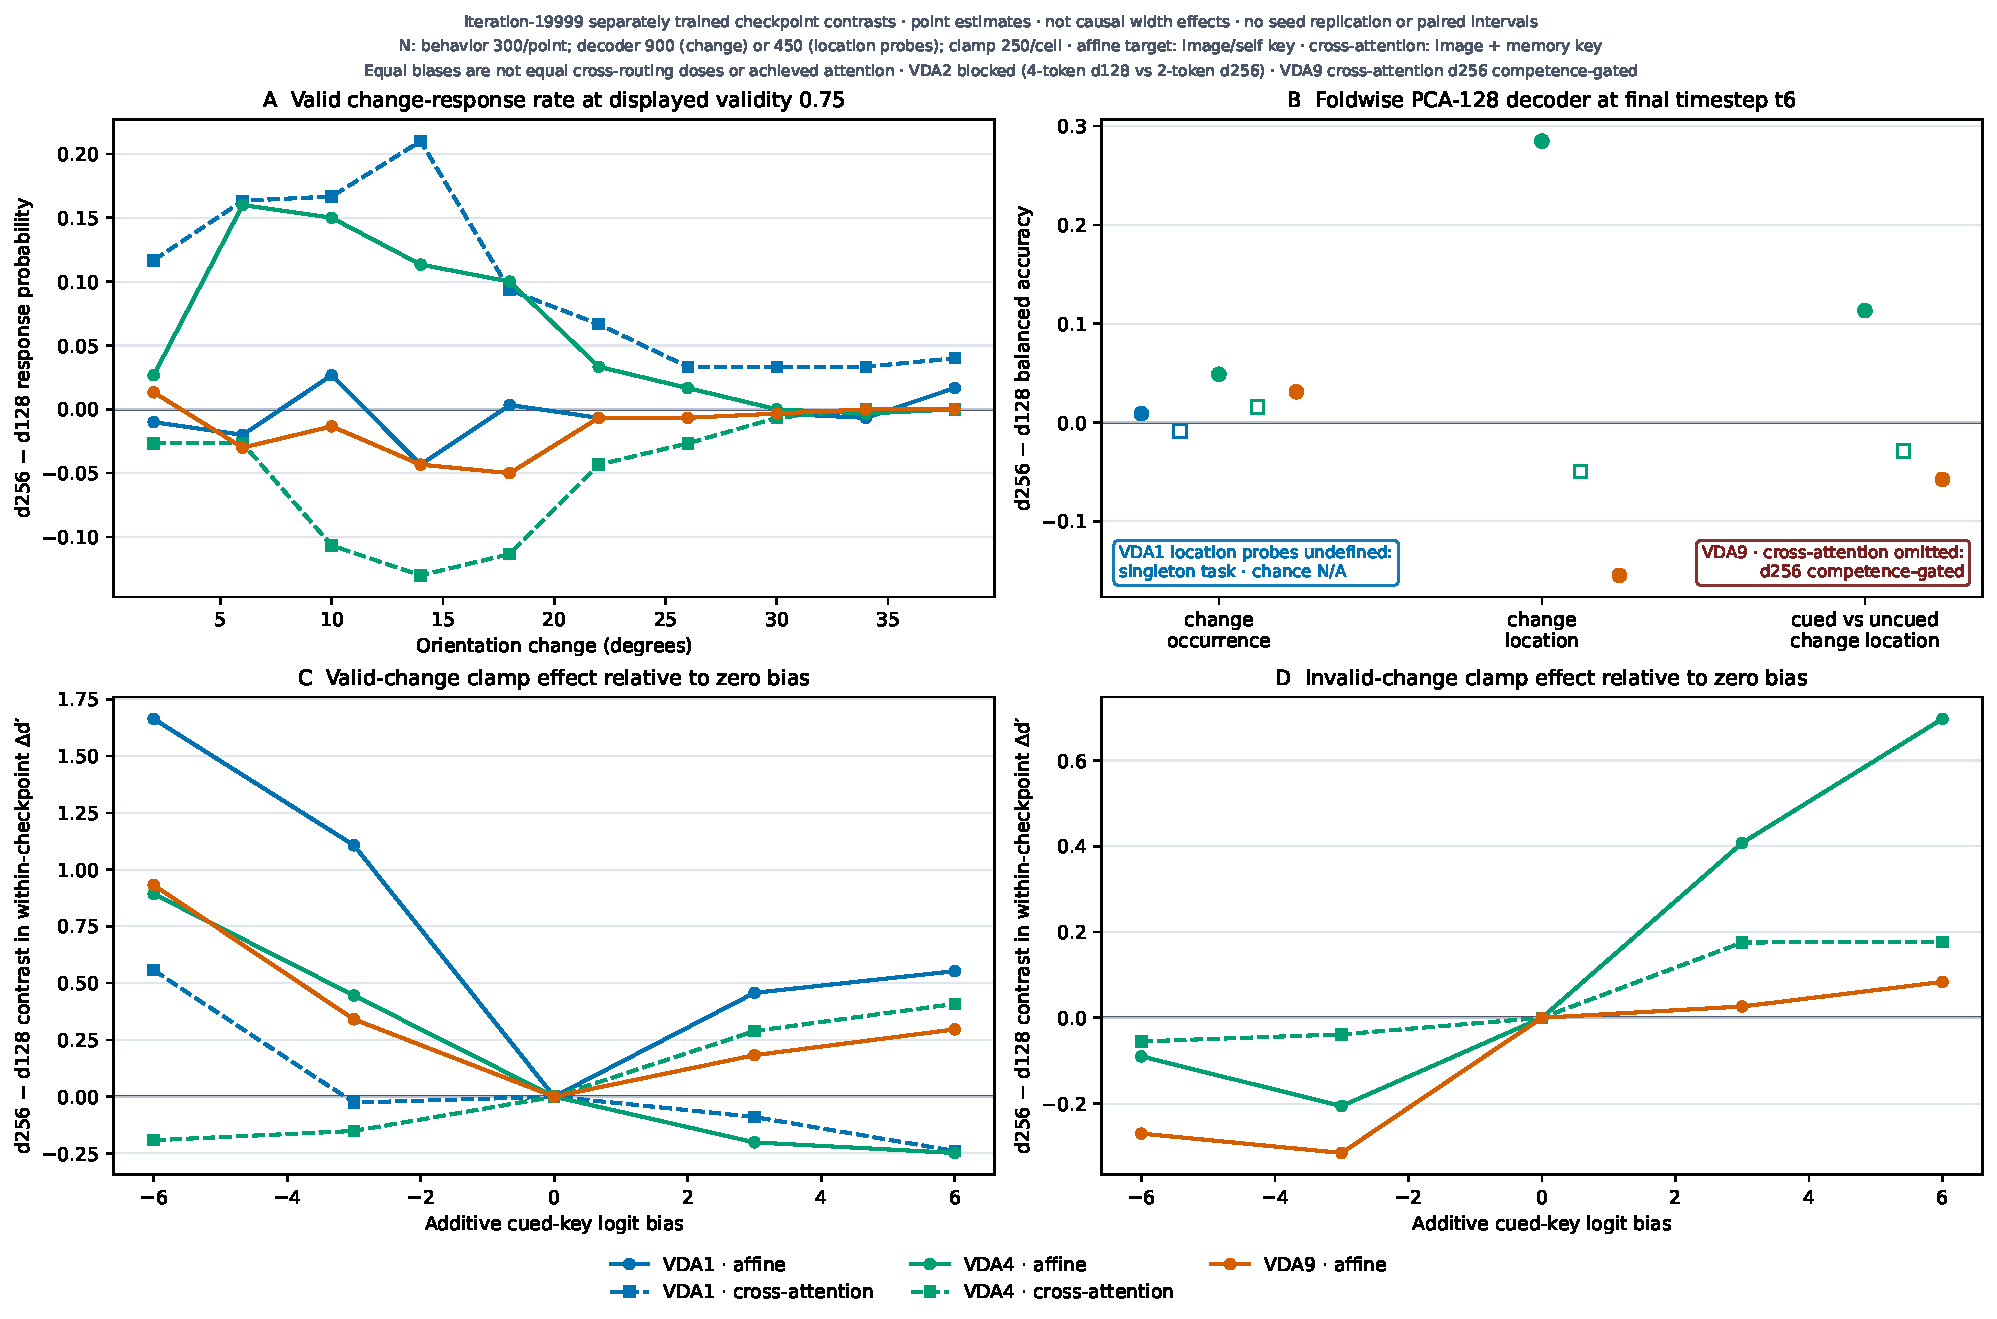
\includegraphics[width=0.68\linewidth]{matched_width_summary.pdf}
\captionof{figure}{\textbf{Matched-width checkpoint summary.} \eclass{Checkpoint-recomputed descriptive and model-intervention evidence.} All ordinates compare separately trained iteration-19999 d256 and d128 checkpoints; across panels, the five admitted pairs do not show a consistent wider-is-better direction. \textbf{Panel map.} A shows valid-location response differences at displayed validity 0.75 (300 trials per point; behavioral, discussed here). B shows t6 foldwise PCA-128 balanced-accuracy differences (representational readout; discussed in Section~\ref{sec:width-decoding}). C and D show cross-checkpoint differences in the within-checkpoint $d'$ change from zero routing-key bias (250 trials per cell; causal intervention, discussed in Section~\ref{sec:existing-intervention}). \textbf{Support.} Unplotted absolute chance is 0.5 for binary change occurrence over 900 trials, 0.25 or $1/9$ for realized location over 450 change-present VDA4 or VDA9 trials, and 0.5 for cued-vs-uncued location over the same 450 trials. Affine routing biases the cued image key only; cross-attention biases that image key and its memory key, so equal nominal biases are not calibrated doses across routing families. VDA1 invalid effects are undefined; VDA2 is blocked by a token-geometry mismatch; VDA9 cross-attention is competence-gated.}\label{fig:matched-width}
\end{center}\end{landscape}

\boundary{The matched-width battery supports checkpoint-specific behavioral point estimates. Across five admitted pairs, the d256-minus-d128 differences do not share one direction, and the design cannot determine whether that variation reflects architecture, training-run variation, or finite evaluation noise. It does not estimate a causal width effect, human working-memory capacity, or training-seed replication.}

\subsection{VDA16: the payoff of a larger, fully controlled set size}\label{sec:vda16-behavior}
Two controlled VDA16 checkpoints -- fixed $4\times4$ grid, sixteen active tokens, $d_\mathrm{mem}=128$, memory decay 1.0, training seed 0 -- reached terminal iteration 19{,}999 and passed the VDA16 production validation gate (contiguous training metrics, checkpoint and producer hashes, frozen inputs, deterministic analysis caches, source-graph checks). The cross-attention checkpoint ended with late-50 rolling correctness 0.774 and remained at $\theta=65^\circ$. The affine checkpoint ended with late-50 rolling correctness 0.845 and advanced from $65^\circ$ to $47^\circ$. Neither reached the declared $8^\circ$ curriculum floor, so both are admitted as \emph{competence-gated} diagnostics, not evidence of convergence, a capacity boundary, or training-population performance. The affine run was statefully resumed from its atomic iteration-17{,}699 checkpoint after an interruption; the exact checkpoint-bound producer snapshot was recovered by its saved hashes, and the terminal bundle records the parent checkpoint identity and resume phase.

At displayed validity 0.75 and the sampled orientation change nearest $18^\circ$, qualifying response rates were \textbf{0.653 for valid changes and 0.133 for forced-invalid changes, a difference of $+0.520$} -- from one frozen checkpoint, finite evaluation trials, not training-seed uncertainty (Figure~\ref{fig:vda16-summary}A). A second, independent rerun that fixes a 100\%-valid cue at top-left S1 and forces the physical change either at S1 or at the opposite corner S16 (300 trials per magnitude and location, common random numbers so the two conditions are pixel-identical through the pre-change frame) reproduces the same pattern with an unambiguous ceiling comparison: at the prespecified $30^\circ$ focal change, the qualifying response rate was \textbf{0.983 for a change at cued S1 and 0.490 for a forced change at S16}, with conditional mean response frames of 5.197 and 5.959 respectively (attentional detail and the full time course are in Section~\ref{sec:vda16-attention-dynamics}, Figure~\ref{fig:vda16-cued-opposite-summary}A--B).

The affine checkpoint shows the same qualitative cueing pattern but a smaller gap at the registered probe: valid response rate 0.893 versus forced-invalid 0.480, a difference of $+0.413$ (Figure~\ref{fig:vda16-affine-summary}A). Its t6 PCA-128 change decoder is stronger than cross-attention (0.814 vs.\ 0.680), as are its realized-location (0.181 vs.\ 0.098) and cued-vs.-uncued change decoders (0.911 vs.\ 0.749; Figures~\ref{fig:vda16-affine-summary}B and \ref{fig:vda16-method-context}B--C). The eight-curve overlays in Figure~\ref{fig:vda16-valid-invalid-overlay} expose the complete displayed-validity series for both response probability and conditional response timing: affine cue-proportion curves are nearly coincident within each location condition, whereas cross-attention shows a pronounced cue-proportion dependence, particularly for forced-invalid response probability. These are separately trained, single-seed checkpoints with different achieved curricula, so the routing-family difference is descriptive rather than causal.

\begin{landscape}\thispagestyle{plain}\begin{center}

\includegraphics[width=0.86\linewidth]{vda16_manuscript_summary.pdf}
\captionof{figure}{\textbf{VDA16 cross-attention analysis.} \eclass{Checkpoint-recomputed, competence-gated evaluation.} Panel A shows matched-bank response rates (behavioral, discussed here). Panel B shows foldwise train-only PCA-128 decoding from recurrent state (representational, Section~\ref{sec:vda16-attention-dynamics}). Panels C--D show sensitivity and criterion under additive cued-location routing-key bias (causal intervention, Section~\ref{sec:existing-intervention}). The checkpoint reached iteration 19{,}999 but remained at $\theta=65^\circ$; d256, decay-contrast, and replicated-seed cells are not admitted.}\label{fig:vda16-summary}
\end{center}\end{landscape}

\begin{landscape}\thispagestyle{plain}\begin{center}
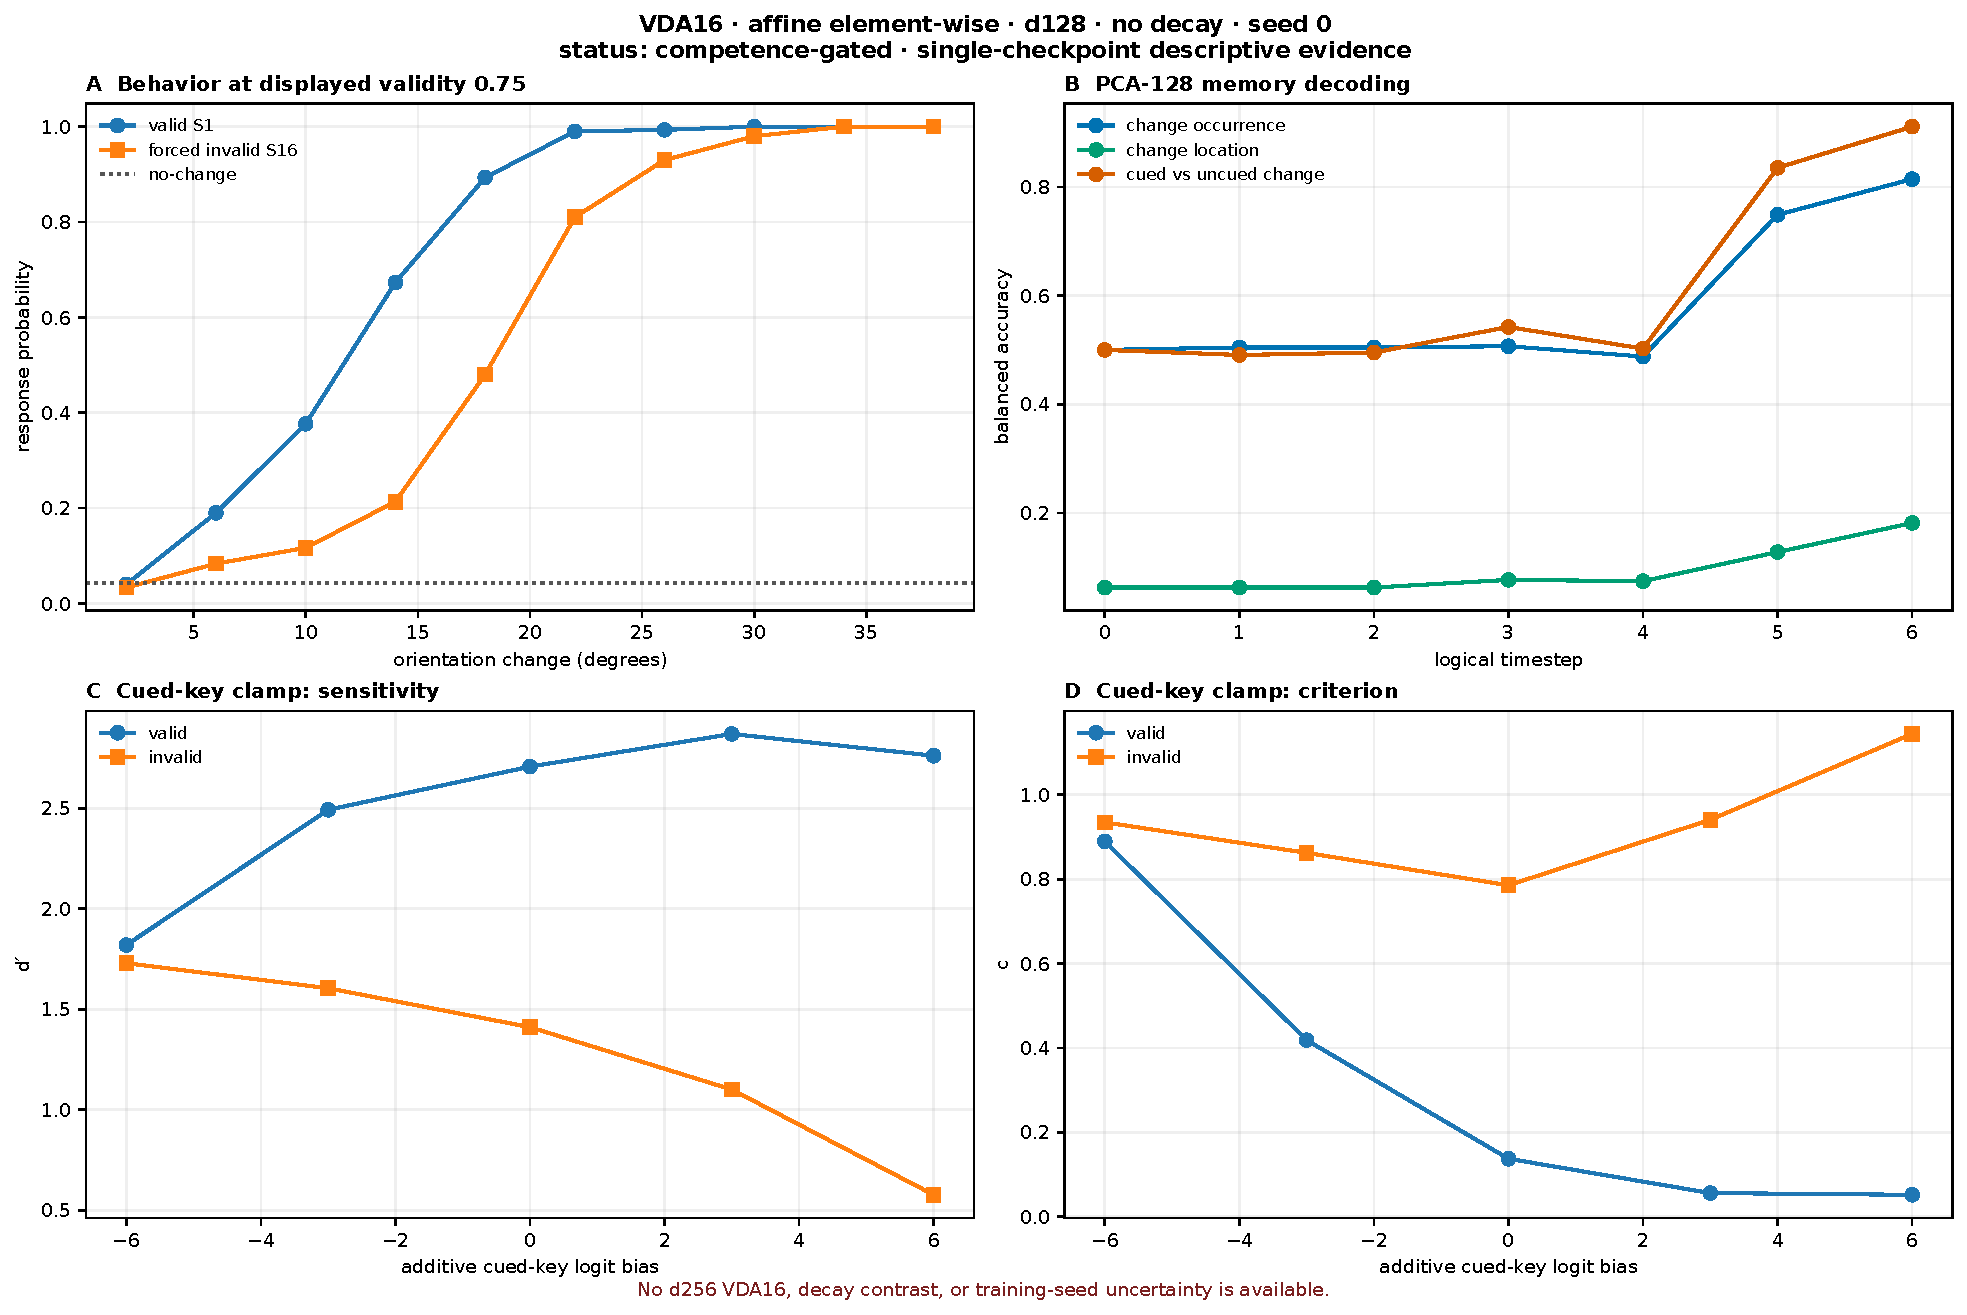
\includegraphics[width=0.86\linewidth]{vda16_affine_manuscript_summary.pdf}
\captionof{figure}{\textbf{VDA16 affine element-wise analysis.} \eclass{Checkpoint-recomputed, competence-gated evaluation.} The panel map and registered trial banks match Figure~\ref{fig:vda16-summary}. Affine routing applies the cued-key bias to its single self-attention key, whereas cross-attention biases the corresponding image and recurrent-memory keys; equal nominal biases are therefore not calibrated cross-family doses. The checkpoint reached iteration 19{,}999 and $\theta=47^\circ$.}\label{fig:vda16-affine-summary}
\end{center}\end{landscape}

\begin{landscape}\thispagestyle{plain}\begin{center}
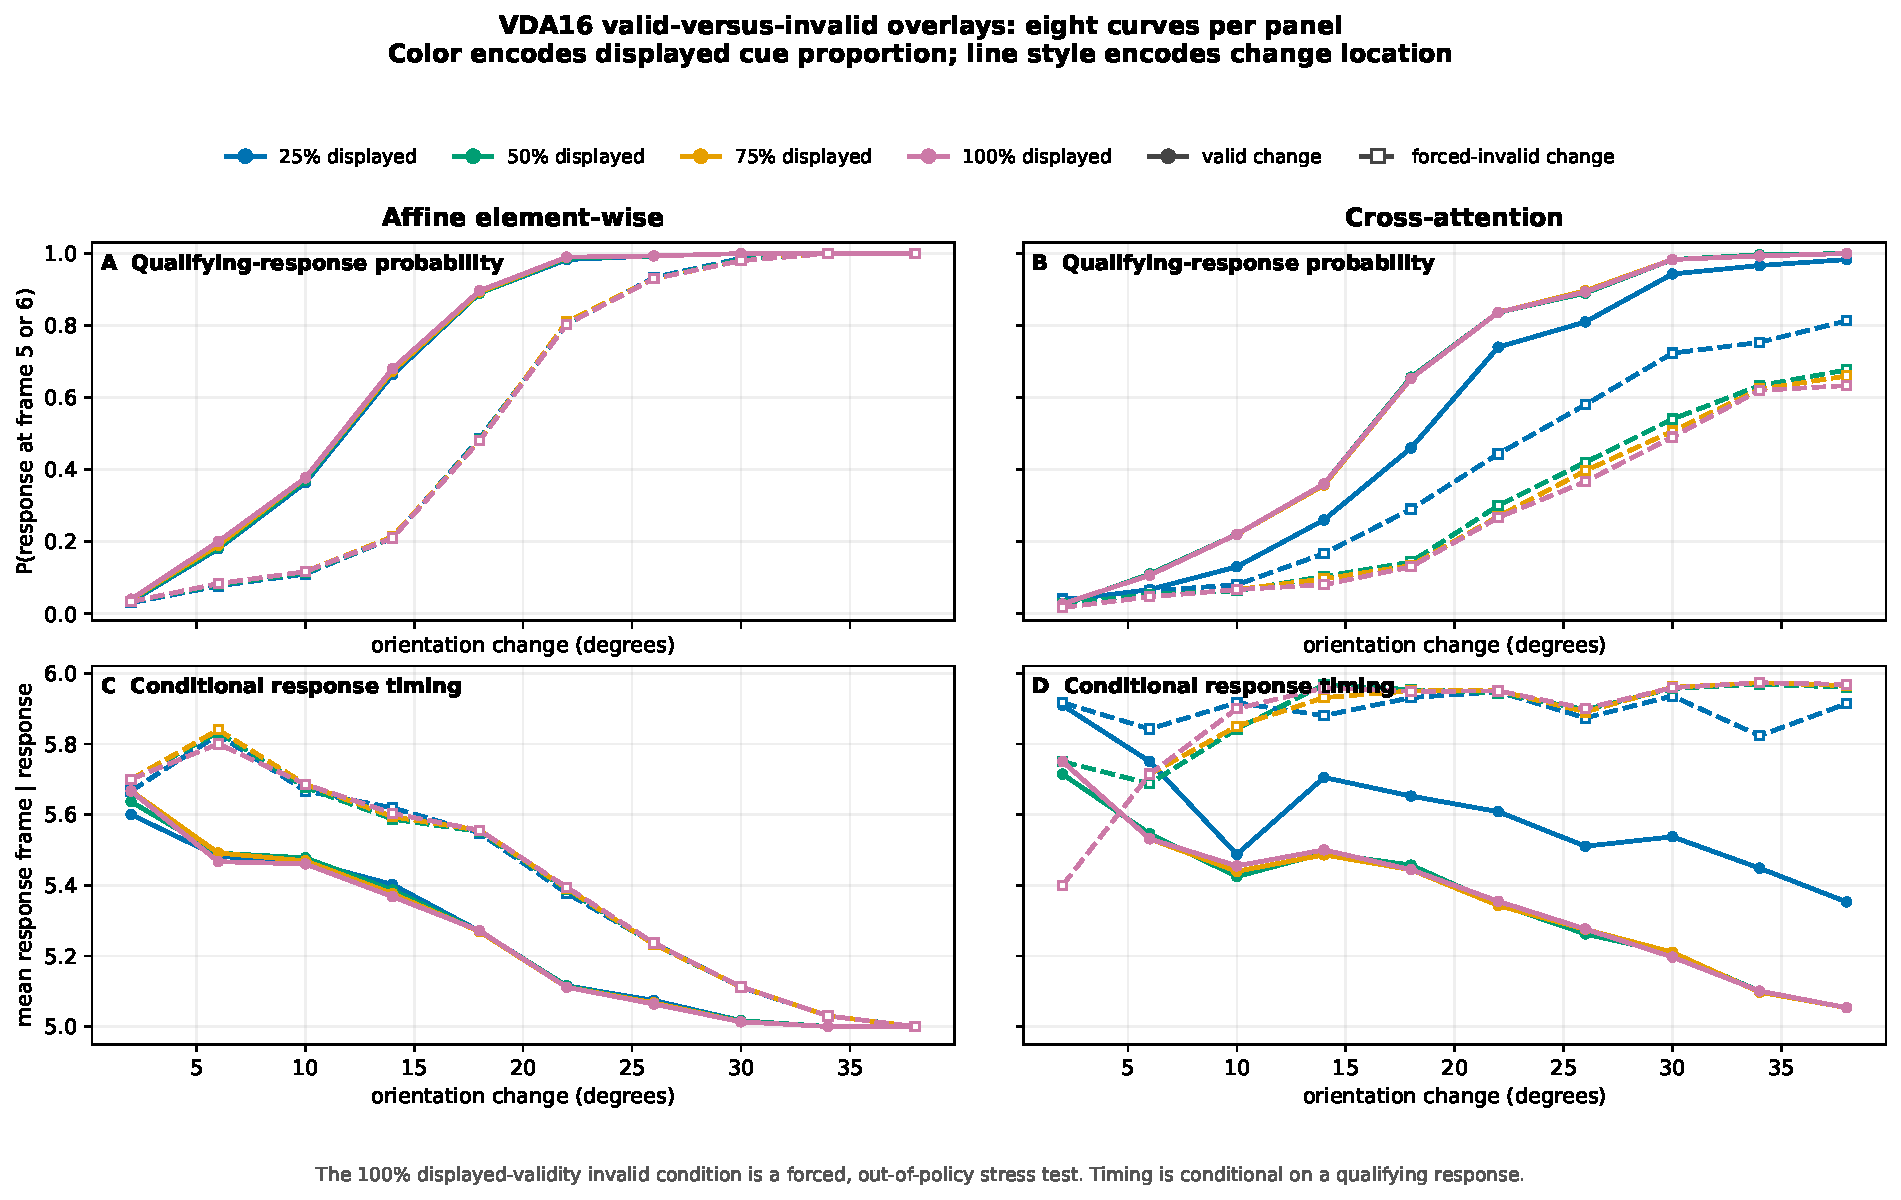
\includegraphics[width=0.80\linewidth]{vda16_valid_invalid_eight_curve_overlay.pdf}
\captionof{figure}{\textbf{VDA16 valid-versus-invalid eight-curve overlays.} \eclass{Checkpoint-recomputed, competence-gated evaluation from matched frozen trial banks.} Each panel overlays four displayed cue proportions (25\%, 50\%, 75\%, 100\%) for valid changes at S1 (solid circles) and forced-invalid changes at S16 (dashed open squares). The top row shows qualifying-response probability; the bottom row shows mean response frame conditional on a qualifying response. The invalid condition at 100\% displayed validity is a forced, out-of-policy stress test. Separate single-seed checkpoints and different achieved curriculum angles preclude a causal routing-family comparison.}\label{fig:vda16-valid-invalid-overlay}
\end{center}\end{landscape}

\subsection{Logistic psychometric functions and chronometric functions across set size}\label{sec:psychometric-fits}
The panels above show raw response probability connected by lines. To ask how large the cueing benefit is in a way that is comparable across set size, we fit a four-parameter logistic $p(x)=\gamma+(1-\gamma-\lambda)/(1+e^{-(x-\alpha)/\beta})$ -- threshold $\alpha$, slope $\beta$, guess rate $\gamma$, lapse rate $\lambda$ -- to the same checkpoint-recomputed response-probability arrays behind Sections~\ref{sec:first-wave-behavior} and \ref{sec:vda16-behavior} (VDA4 and VDA9, both routing families, and both VDA16 checkpoints; weighted least squares, binomial-variance weights, 300 trials per point). This is a re-analysis of already-cached, already-verified data: no checkpoint is re-run to produce it.

At displayed validity 0.75, the fitted threshold for cross-attention shifts from $12.0^\circ$ (change at cued location) to $17.3^\circ$ (change at the opposite location) at set size 4 -- a $5.3^\circ$ shift -- and from $16.0^\circ$ to $26.9^\circ$ at set size 16, a $10.9^\circ$ shift, roughly double (Figure~\ref{fig:psych-fit-vda4-cross}, Figure~\ref{fig:psych-fit-vda16}). The threshold-vs.-validity panels (Figure~\ref{fig:psych-fit-vda4-cross}B, Figure~\ref{fig:psych-fit-vda16}B) show this is not an artifact of one displayed-validity level: as displayed validity rises from 0.25 to 1.0, the valid-location threshold falls while the invalid-location threshold rises, at both set sizes, and the two curves separate more, and from a larger baseline gap, at set size 16.

The affine checkpoint does not reproduce this widening as cleanly. Its fitted threshold shift grows from $3.4^\circ$ at set size 4 ($11.6^\circ$ to $15.0^\circ$) to $6.5^\circ$ at set size 9 ($11.5^\circ$ to $18.0^\circ$), then is essentially flat into set size 16 at $6.2^\circ$ ($11.8^\circ$ to $18.0^\circ$; Figure~\ref{fig:psych-fit-vda16-affine}) -- close to affine's own set-size-9 shift and well short of cross-attention's $10.9^\circ$ at the same set size. The raw valid-minus-invalid gap near $18^\circ$ tells the same story: for cross-attention it grows monotonically across the historical-to-controlled ladder ($0.27$ at set size 4, $0.32$ at set size 9, $0.44$ at set size 16), but for affine it rises then is flat-to-falling ($0.19$, $0.38$, $0.32$) -- set size 16 is not affine's largest gap, set size 9 is. The cross-environment summary (Figure~\ref{fig:psych-fit-summary}) plots both VDA16 checkpoints as open, unconnected points, following the same convention as Figure~\ref{fig:vda16-method-context}: historical VDA4 and VDA9 share one interchangeable lineage, but controlled VDA16 comes from a separately frozen executable and runtime lineage, so this is a descriptive juxtaposition across single checkpoints, not a fitted capacity law. \textbf{The growing-cueing-gap-with-set-size pattern that motivates this whole manuscript therefore holds cleanly within the cross-attention lineage but not within the affine lineage} -- it is at least as much a property of which routing family is asked as it is a property of set size alone, a routing-family analogue of Section~\ref{sec:width-behavior}'s finding that a wider recurrent state does not consistently produce a larger cueing benefit.

\begin{landscape}\thispagestyle{plain}\begin{center}
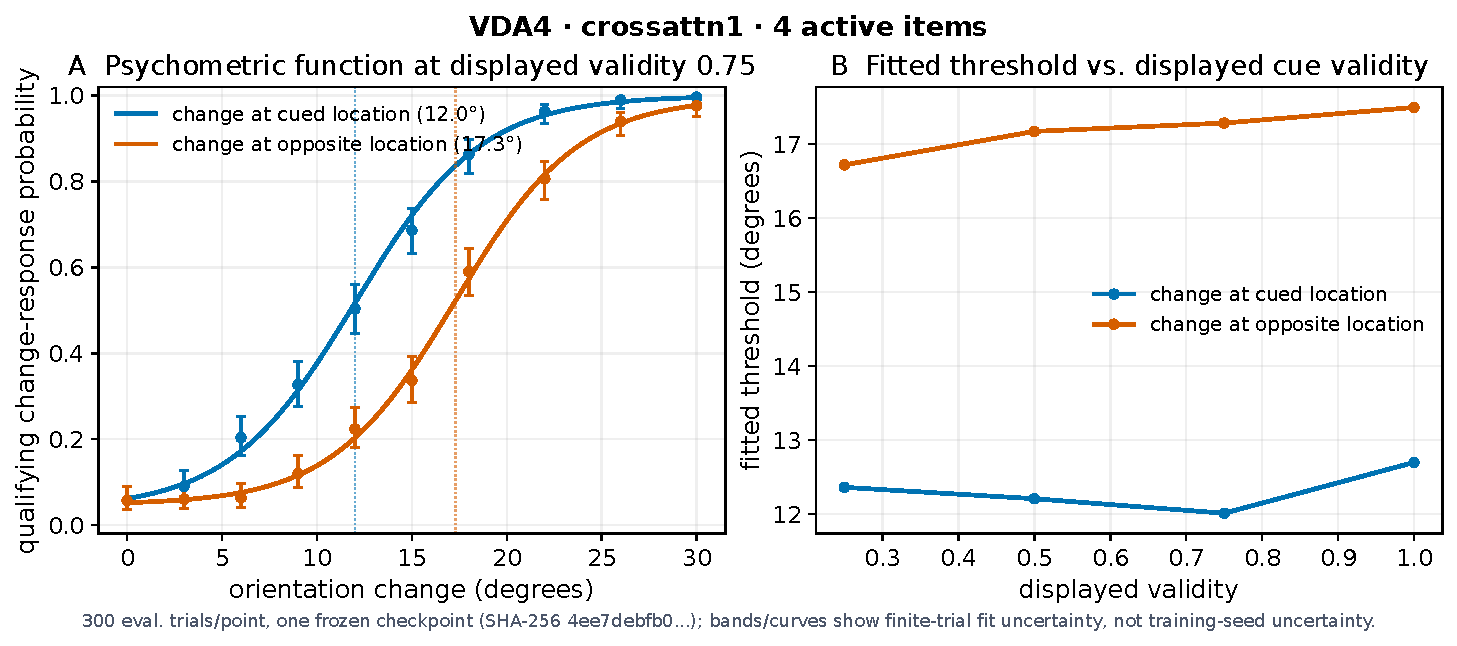
\includegraphics[width=0.92\linewidth]{psychometric_fit_vda4_crossattn1.pdf}
\captionof{figure}{\textbf{VDA4 logistic psychometric fits, cross-attention.} \eclass{Re-analysis of checkpoint-recomputed cached data; no checkpoint re-run.} Panel A: fitted psychometric functions at displayed validity 0.75 with Wilson-interval data points. Panel B: fitted threshold vs.\ displayed validity, by location condition. Threshold is the logistic inflection point in degrees.}\label{fig:psych-fit-vda4-cross}
\end{center}\end{landscape}

\begin{landscape}\thispagestyle{plain}\begin{center}
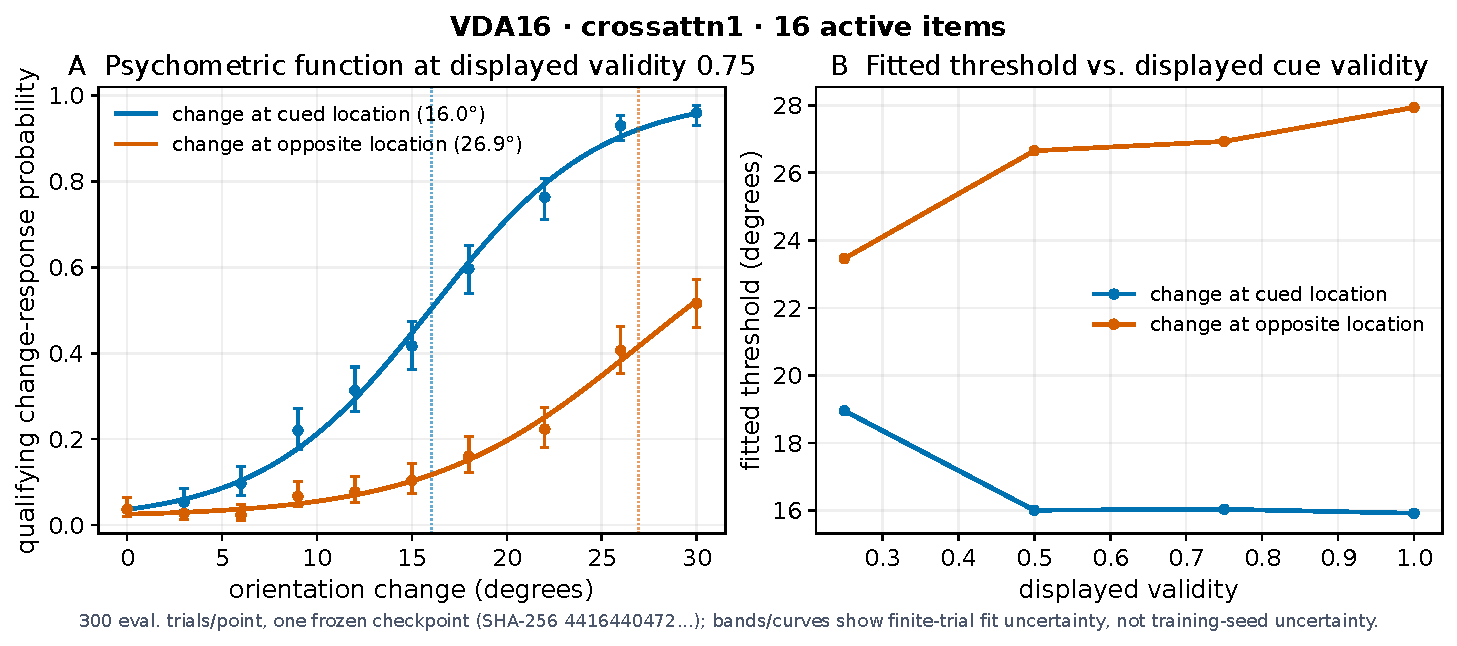
\includegraphics[width=0.92\linewidth]{psychometric_fit_vda16_crossattn1.pdf}
\captionof{figure}{\textbf{VDA16 logistic psychometric fits, cross-attention.} \eclass{Re-analysis of checkpoint-recomputed cached data; competence-gated; no checkpoint re-run.} Same layout as Figure~\ref{fig:psych-fit-vda4-cross}. The valid-vs-invalid threshold separation is roughly double the set-size-4 separation at every displayed validity level.}\label{fig:psych-fit-vda16}
\end{center}\end{landscape}

\begin{landscape}\thispagestyle{plain}\begin{center}
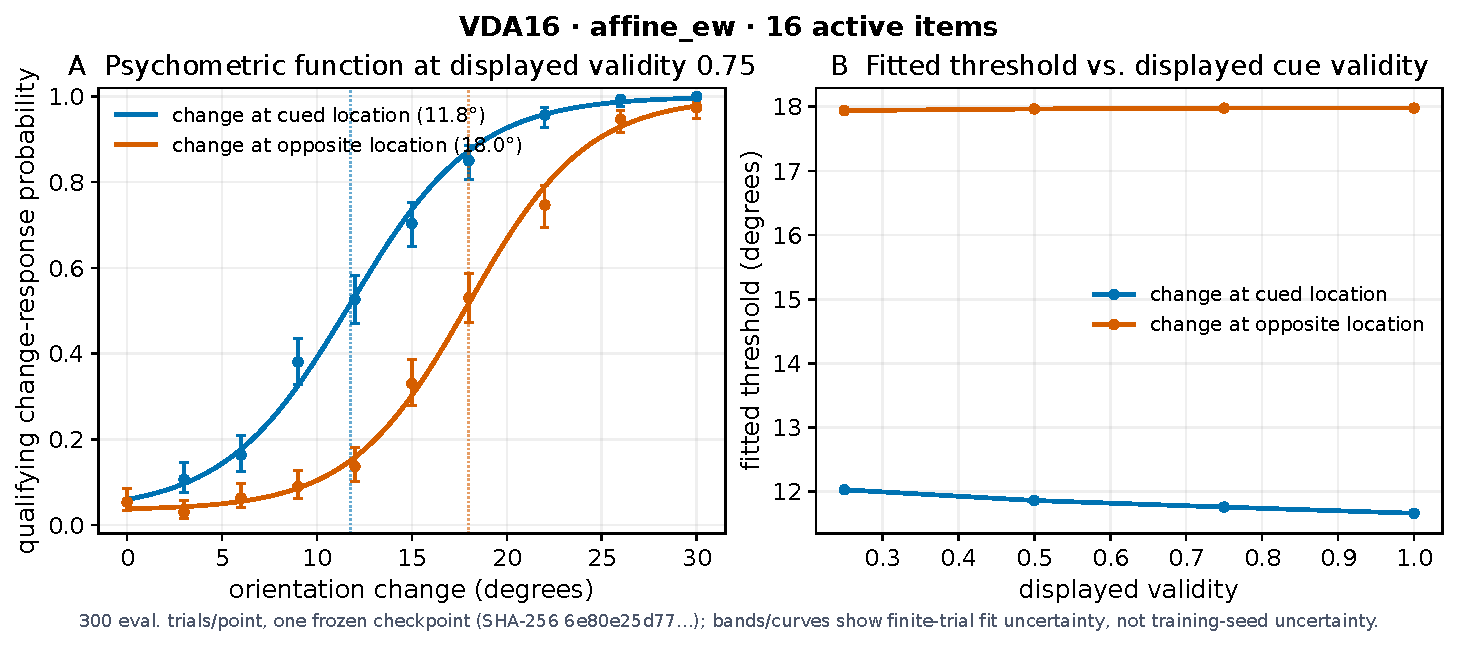
\includegraphics[width=0.92\linewidth]{psychometric_fit_vda16_affine_ew.pdf}
\captionof{figure}{\textbf{VDA16 logistic psychometric fits, affine element-wise.} \eclass{Re-analysis of checkpoint-recomputed cached data; competence-gated; no checkpoint re-run.} Same layout as Figure~\ref{fig:psych-fit-vda4-cross}. Unlike cross-attention (Figure~\ref{fig:psych-fit-vda16}), the affine valid-vs-invalid threshold separation at set size 16 is comparable to its own separation at set size 4, not roughly double it.}\label{fig:psych-fit-vda16-affine}
\end{center}\end{landscape}

\begin{center}
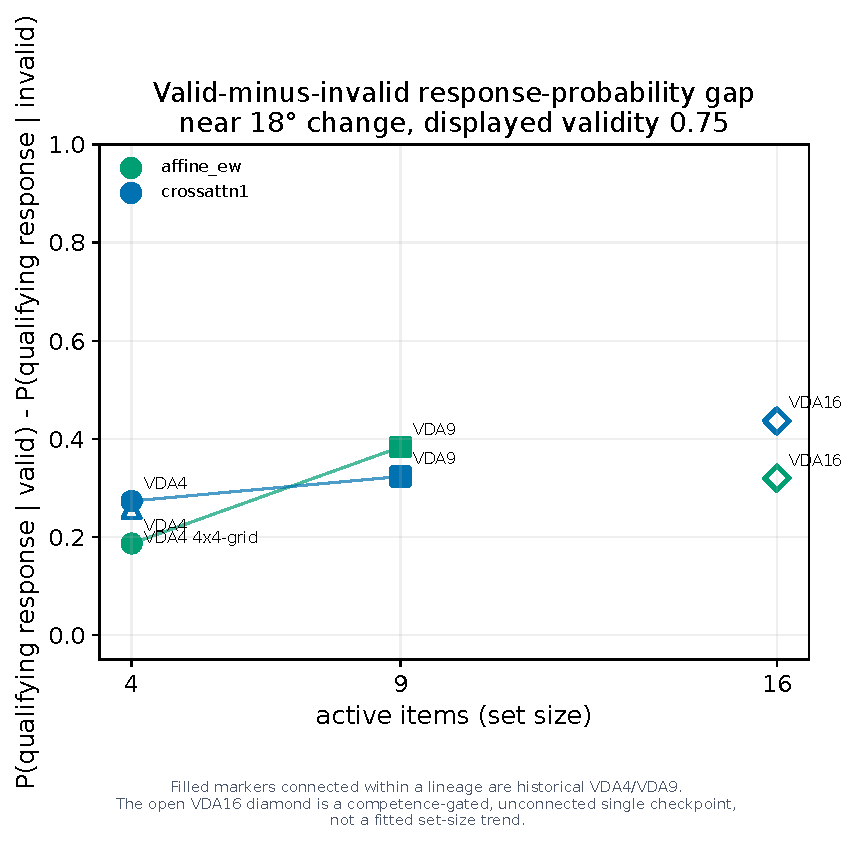
\includegraphics[width=0.62\linewidth]{psychometric_fit_setsize_summary.pdf}
\captionof{figure}{\textbf{Cueing-effect magnitude vs.\ set size.} \eclass{Re-analysis of checkpoint-recomputed cached data across environments.} Valid-minus-invalid qualifying-response-probability gap near an $18^\circ$ change, at displayed validity 0.75. Filled markers connected within a lineage are historical VDA4/VDA9; the two open VDA16 diamonds (cross-attention and affine) are competence-gated, differently lineaged single checkpoints plotted as unconnected points, matching Figure~\ref{fig:vda16-method-context}. Fits for VDA4 and VDA9 (both routing families) are in the companion figure directory \texttt{reports/vda\_series/figures/psychometric\_fits/}.}\label{fig:psych-fit-summary}
\end{center}

\begin{center}

\includegraphics[width=0.92\linewidth]{vda_method_comparison_with_vda16.pdf}
\captionof{figure}{\textbf{Descriptive d128 routing-family context with both VDA16 checkpoints.} \eclass{Cross-lineage contextual comparison.} Panel A shows valid-minus-invalid response rate; Panels B--C show final-timestep decoders; Panel D shows no-change false-alarm rate. Open, unconnected VDA16 markers are competence-gated and do not belong to fitted set-size trends. The affine and cross-attention checkpoints were trained separately and reached different curriculum angles ($47^\circ$ and $65^\circ$), so their separation is descriptive, not a causal routing-family effect. VDA2 is omitted because no compatible modern matched-width shard exists.}\label{fig:vda16-method-context}
\end{center}

Panel D of Figure~\ref{fig:vda16-method-context} shows the no-change qualifying false-alarm rate is low and does not rise with set size, which weighs against the simplest criterion-only account of the widening gap above: if the model were simply becoming more willing to declare ``change'' everywhere as set size grows, false alarms should rise together with valid hits. That is suggestive, not a formal decomposition -- a full sensitivity/criterion separation with an external-noise manipulation, in the sense Carrasco and Luo and Maunsell require before ``attention'' can be assigned to discriminability rather than policy, has been run only for the routing-key intervention in Section~\ref{sec:existing-intervention}, and only there \cite{carrasco2011,luo2018}.

\boundary{The set-size comparison above juxtaposes single checkpoints (two set sizes $\times$ two routing families historically, plus two separately trained VDA16 routing families) from two non-interchangeable lineages under a shared but re-derived analysis (the logistic fit). It is not a controlled, multi-seed set-size series: historical VDA4/VDA9 and controlled VDA16 differ in grid geometry, token count, and training/runtime lineage in addition to active-item count, so growth in the fitted gap is consistent with a set-size effect but does not isolate one, and the fact that only the cross-attention lineage shows monotonic growth suggests routing family is at least as load-bearing as set size for this particular pattern. Section~\ref{sec:discussion} returns to this, including the specific confound between set size and spatial discretization.}

\section{Attention dynamics over time}\label{sec:attention-dynamics}
Behavior alone cannot say whether a cueing benefit comes from where the model looks. This section asks where the model's internal routing weight goes over the full trial timeline -- t0 blank, t1 cue, t2 delay, t3--t4 array, t5 change, t6 response -- as a function of cue validity, and what a held-out probe can read from the recurrent state at each point, following the representational step of Carrasco's and Herman and Krauzlis's programs: align the signal to the event, separate conditions, and only then interpret \cite{carrasco2011,herman2017}. Throughout, ``attention/priority map'' names the model's own routing or gating weights over locations; it is not a claim about a literal neural attention map.

\subsection{Event-aligned attention maps: VDA4 and VDA9}\label{sec:first-wave-attention}
Each attention product evaluates four displayed cue proportions (25\%, 50\%, 75\%, 100\%) using 96 matched deterministic no-change trials per proportion: the cue remains fixed at S1, no orientation change occurs at any location, and t5 is retained only as the nominal change opportunity. Rows encode cue proportion; columns preserve logical timesteps t0--t6. Affine attention has one spatial-key array; cross-attention keeps image and recurrent-memory key groups separate, so it is shown as two cue-proportion-by-time arrays. A red outline marks the fixed S1 cue location, and each figure uses a shared zero-to-observed-maximum scale within itself. These maps ask whether cue proportion modulates routing weight at the nominal change opportunity even with no physical change to detect; because no invalid-change attention contrast is included here, this evidence is partial on its own and is completed by the VDA16 paired experiment in Section~\ref{sec:vda16-attention-dynamics}.

\begin{landscape}\thispagestyle{plain}\begin{center}
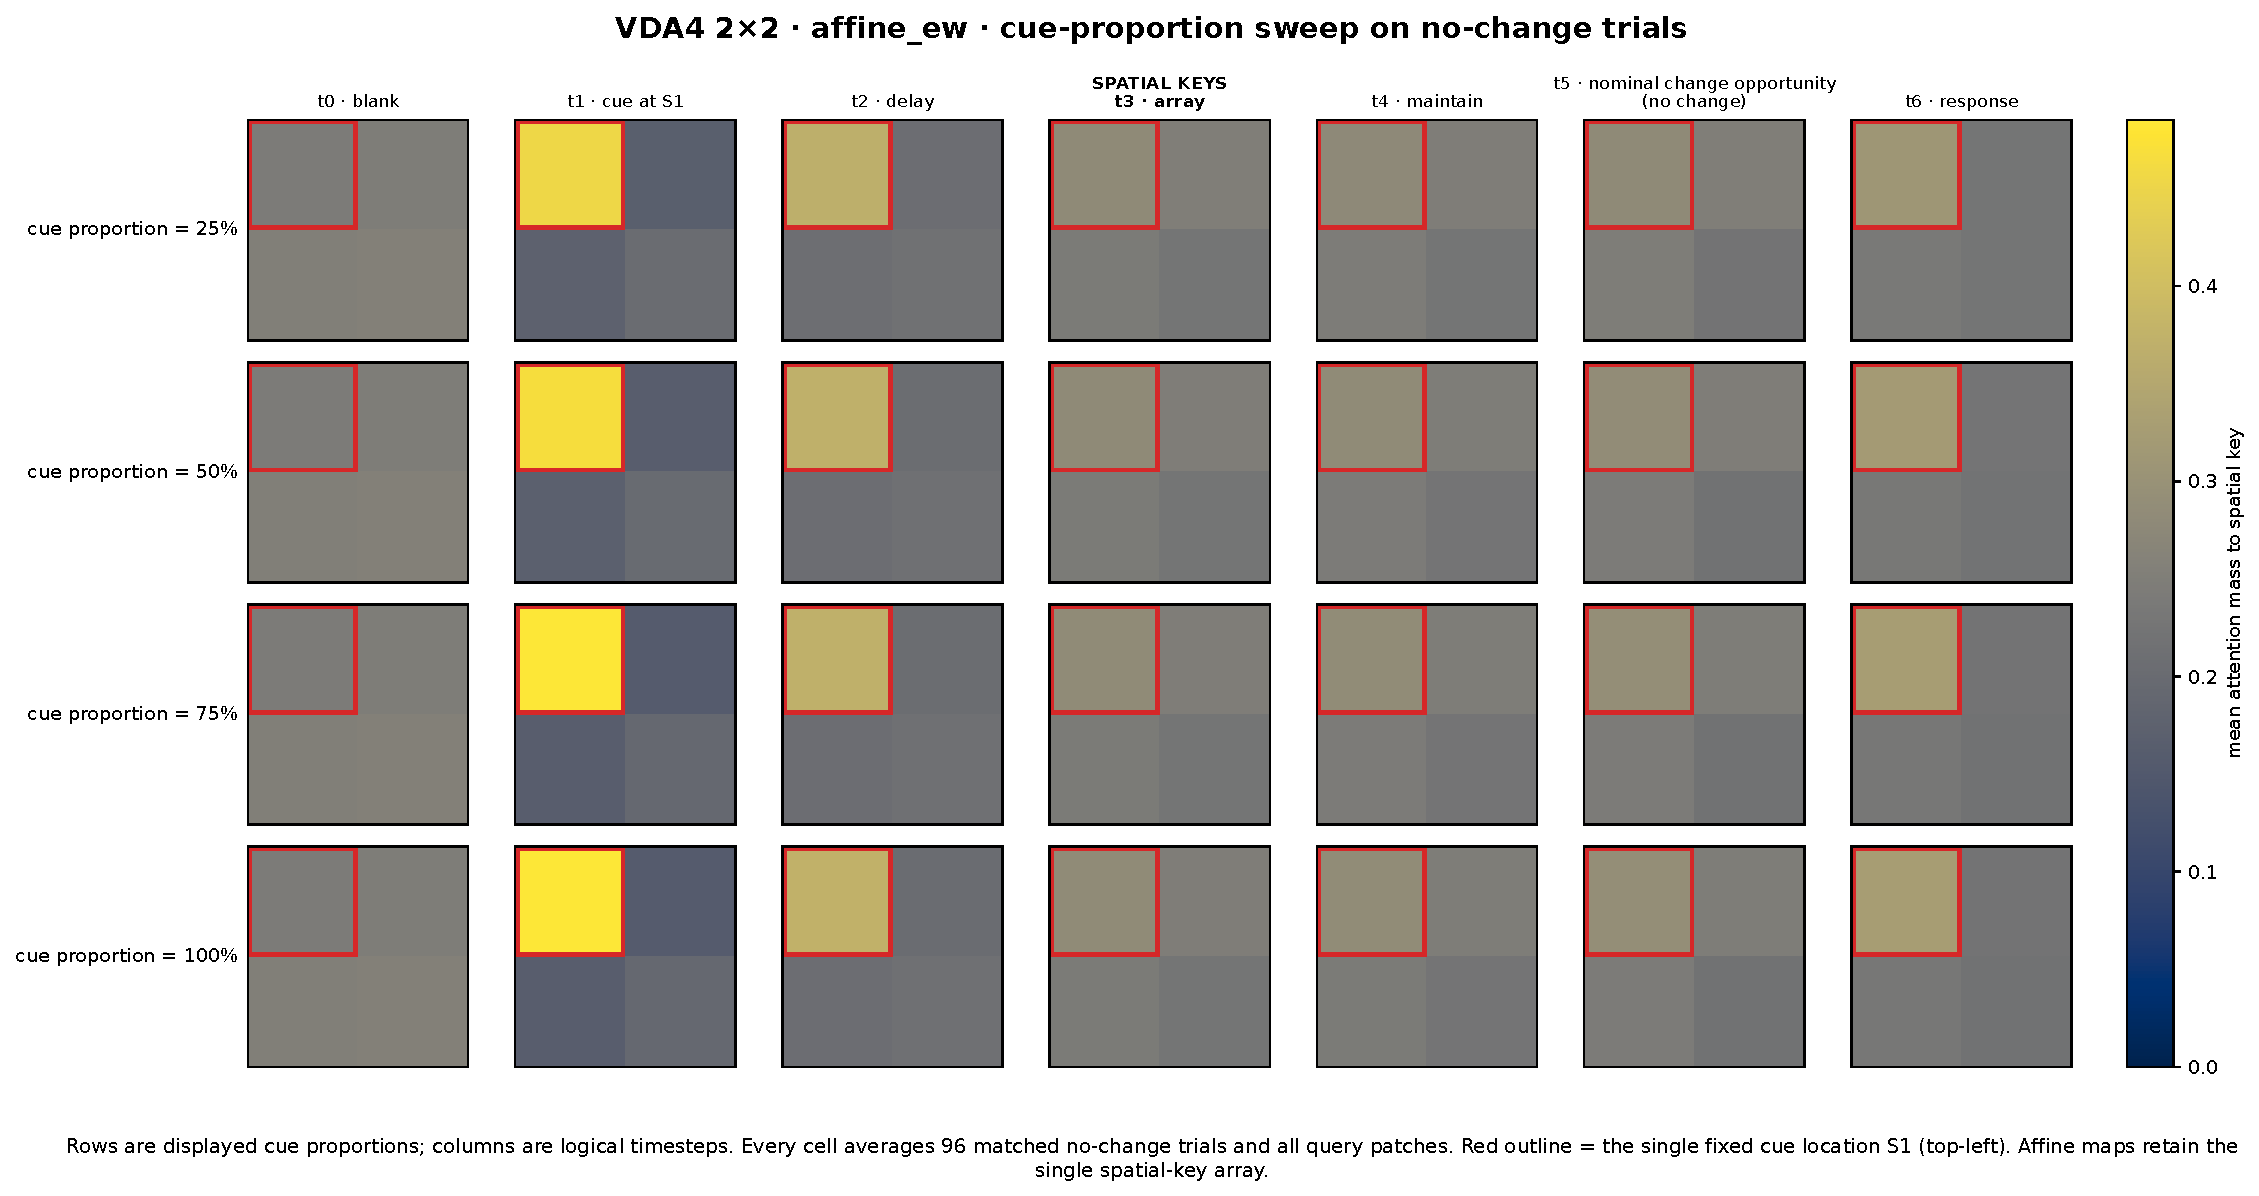
\includegraphics[width=0.96\linewidth]{first_wave_attention_vda4_affine_ew.pdf}
\captionof{figure}{\textbf{VDA4 affine attention on no-change trials.} \eclass{Checkpoint-recomputed descriptive measurement; 96 matched trials per displayed cue proportion.} Rows are cue proportions and columns are logical timesteps. Uniform mass over four spatial keys would assign 0.250 to each location.}\label{fig:first-wave-attn-vda4-affine}
\end{center}\end{landscape}

\begin{landscape}\thispagestyle{plain}\begin{center}
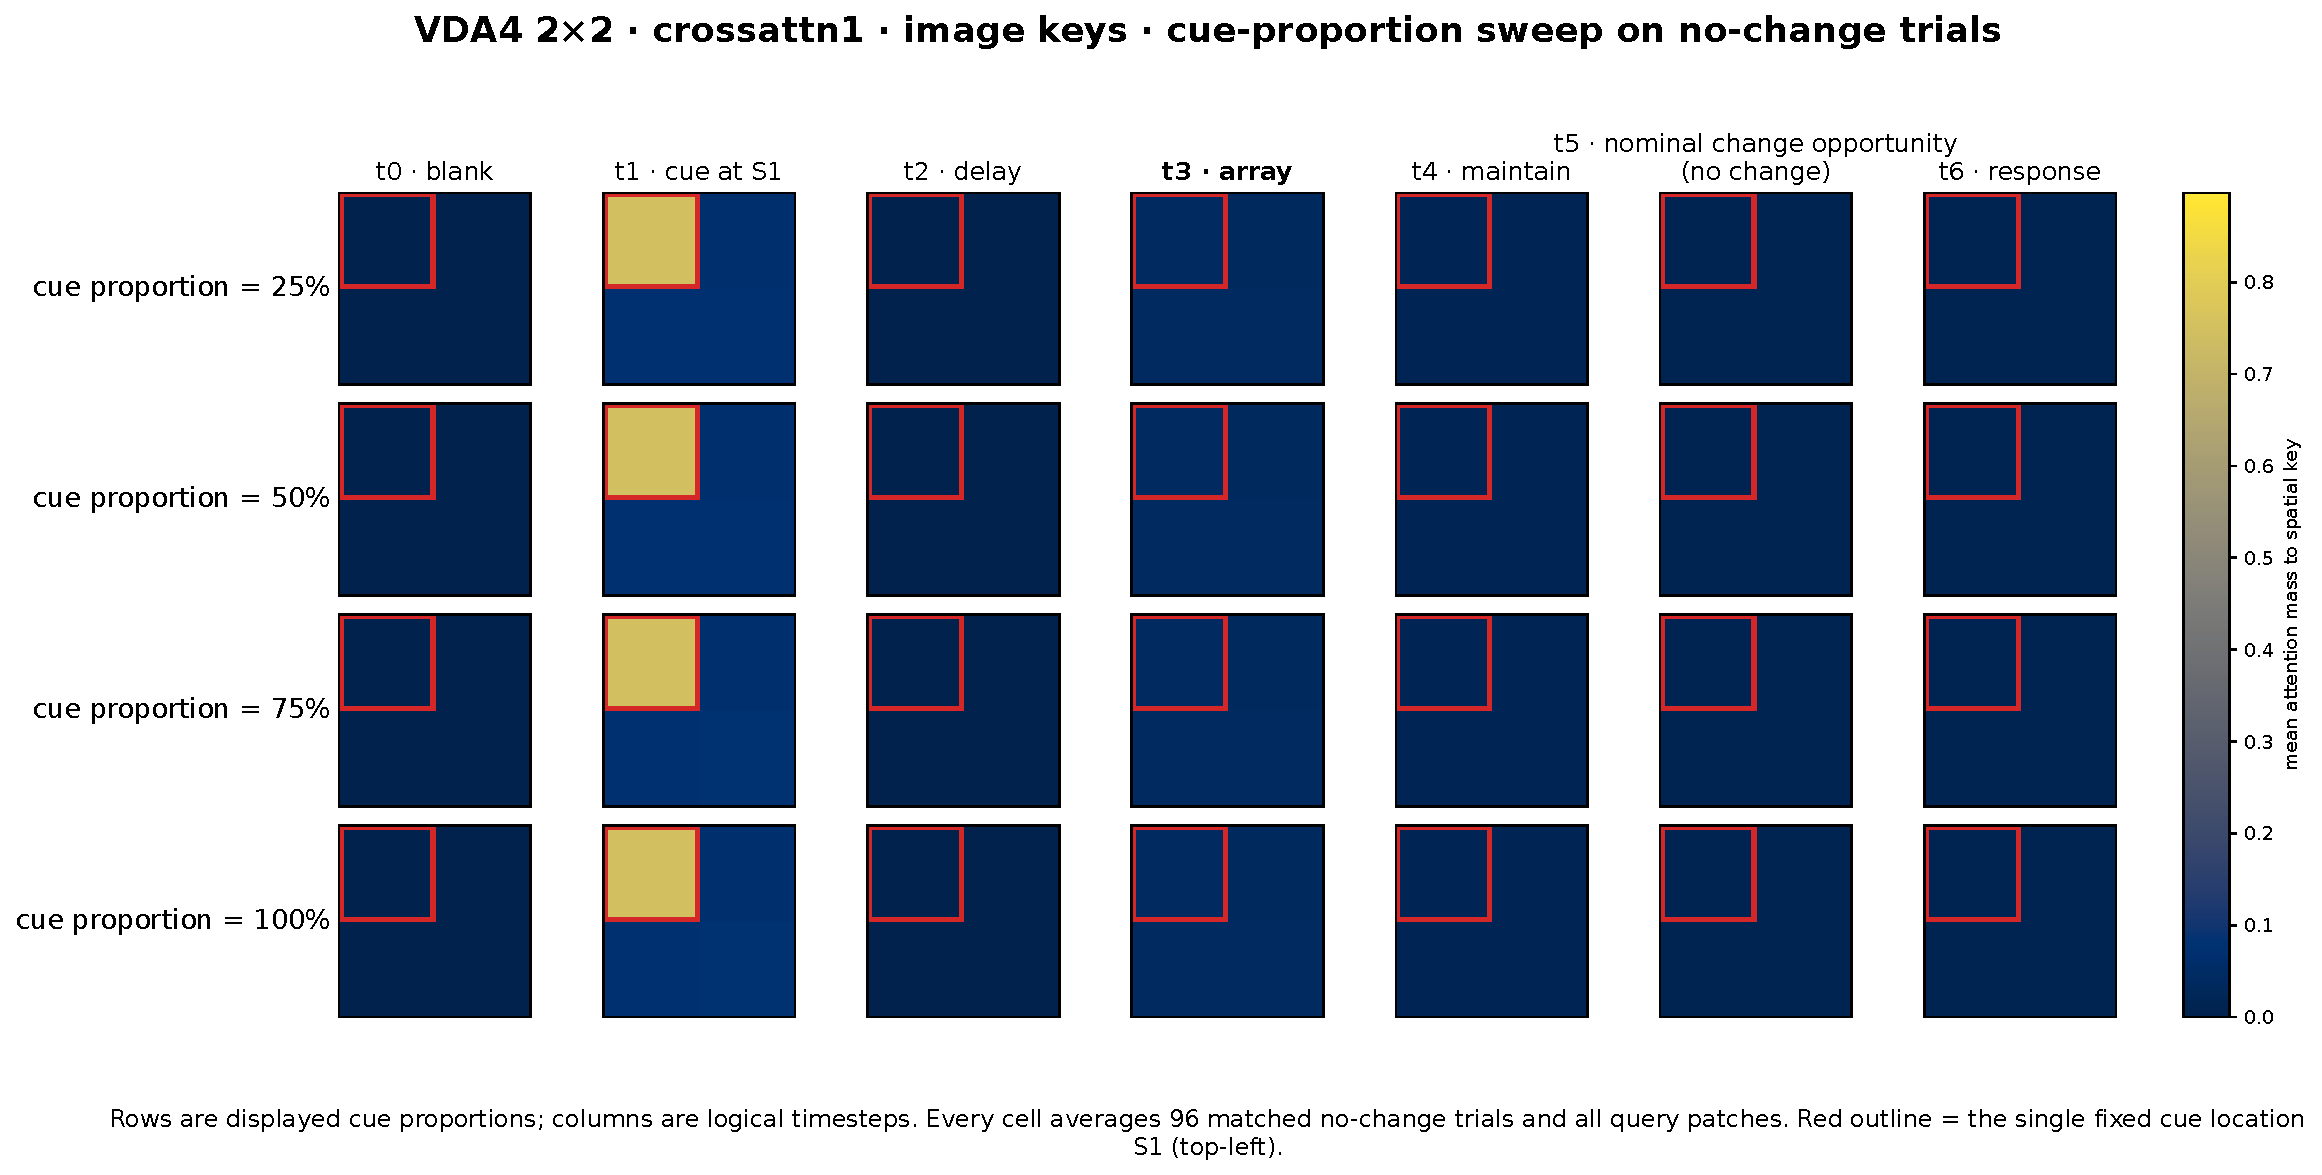
\includegraphics[width=0.96\linewidth]{first_wave_attention_vda4_crossattn1_image_keys.pdf}
\captionof{figure}{\textbf{VDA4 cross-attention to image keys on no-change trials.} \eclass{Checkpoint-recomputed descriptive measurement; 96 matched trials per displayed cue proportion.} Image-key $4\times7$ array. Under uniform mass over all eight cross-attention keys, each spatial key receives $1/8=0.125$.}\label{fig:first-wave-attn-vda4-cross-image}
\end{center}\end{landscape}

\begin{landscape}\thispagestyle{plain}\begin{center}
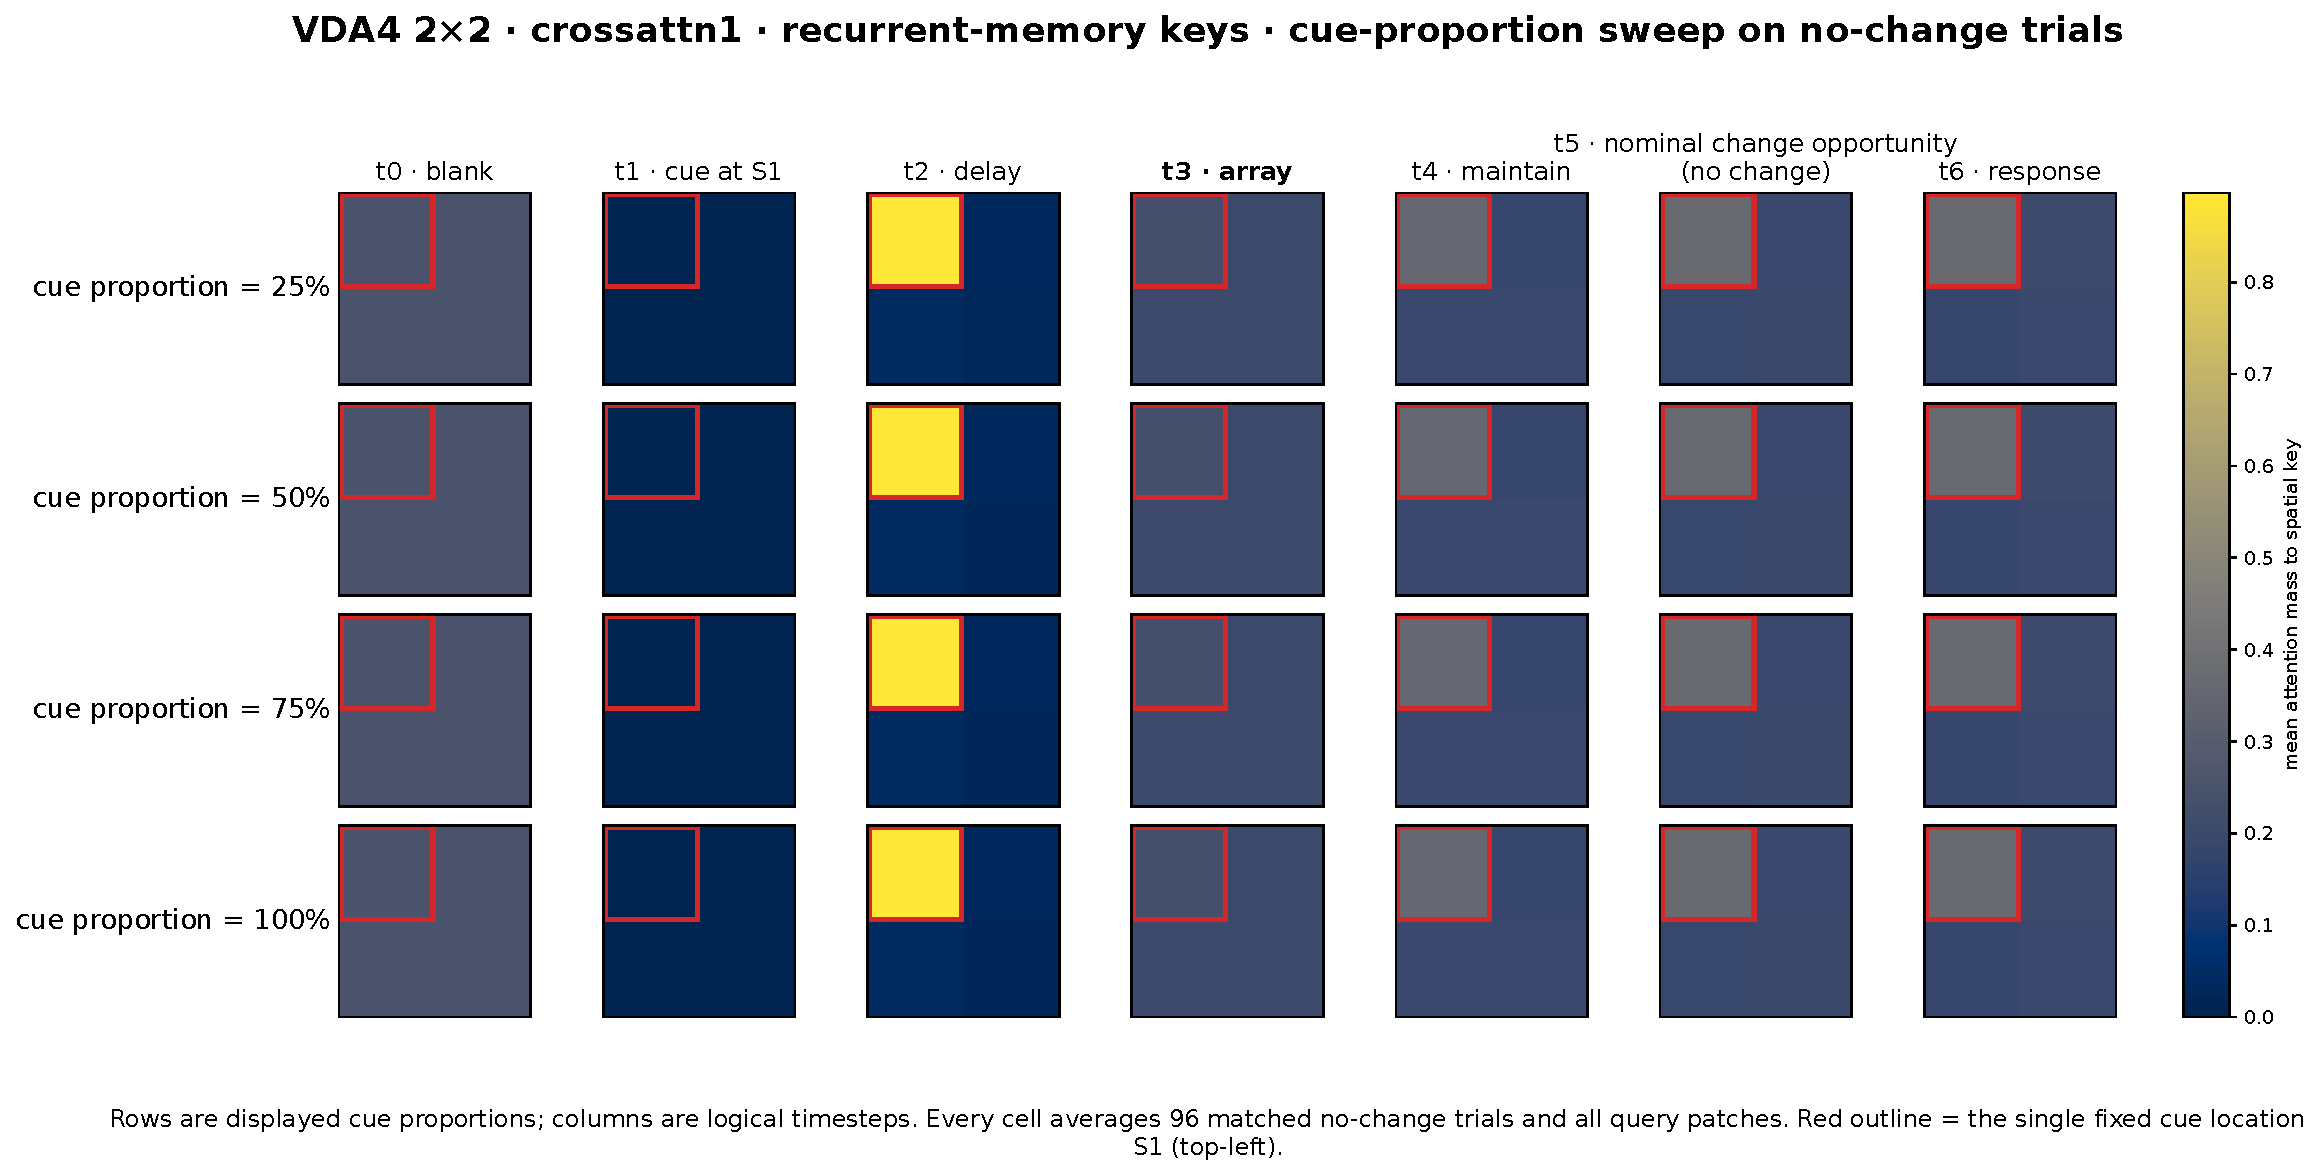
\includegraphics[width=0.96\linewidth]{first_wave_attention_vda4_crossattn1_recurrent_memory_keys.pdf}
\captionof{figure}{\textbf{VDA4 cross-attention to recurrent-memory keys on no-change trials.} \eclass{Checkpoint-recomputed descriptive measurement; 96 matched trials per displayed cue proportion.} Recurrent-memory-key $4\times7$ array, sharing scale with Figure~\ref{fig:first-wave-attn-vda4-cross-image}.}\label{fig:first-wave-attn-vda4-cross}
\end{center}\end{landscape}

\begin{landscape}\thispagestyle{plain}\begin{center}
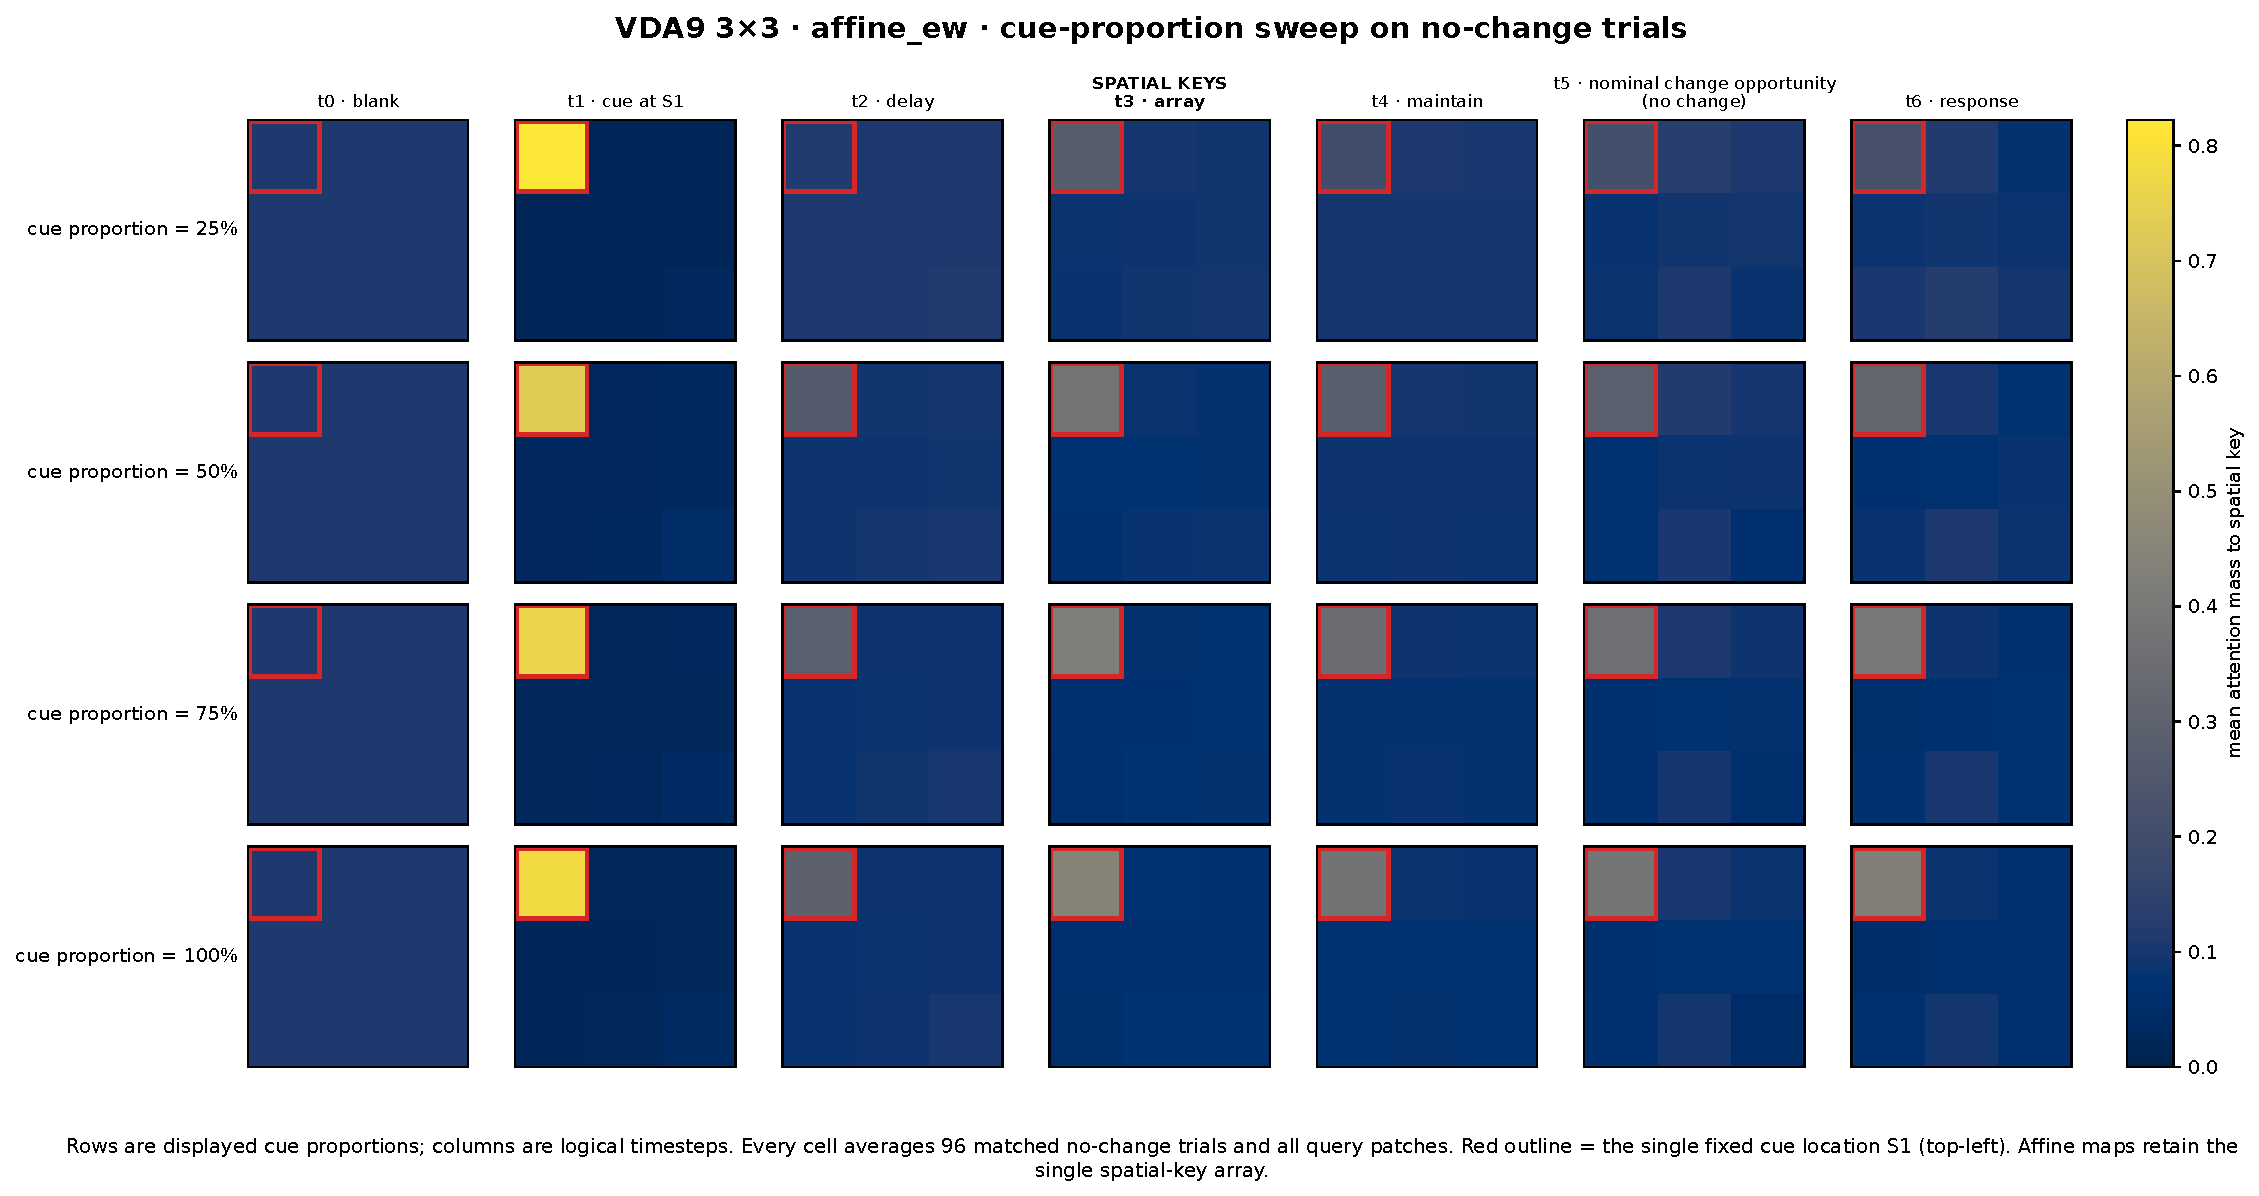
\includegraphics[width=0.96\linewidth]{first_wave_attention_vda9_affine_ew.pdf}
\captionof{figure}{\textbf{VDA9 affine attention on no-change trials.} \eclass{Checkpoint-recomputed descriptive measurement; 96 matched trials per displayed cue proportion.} Uniform mass over nine spatial keys would assign $1/9=0.111\ldots$ to each location.}\label{fig:first-wave-attn-vda9-affine}
\end{center}\end{landscape}

\begin{landscape}\thispagestyle{plain}\begin{center}
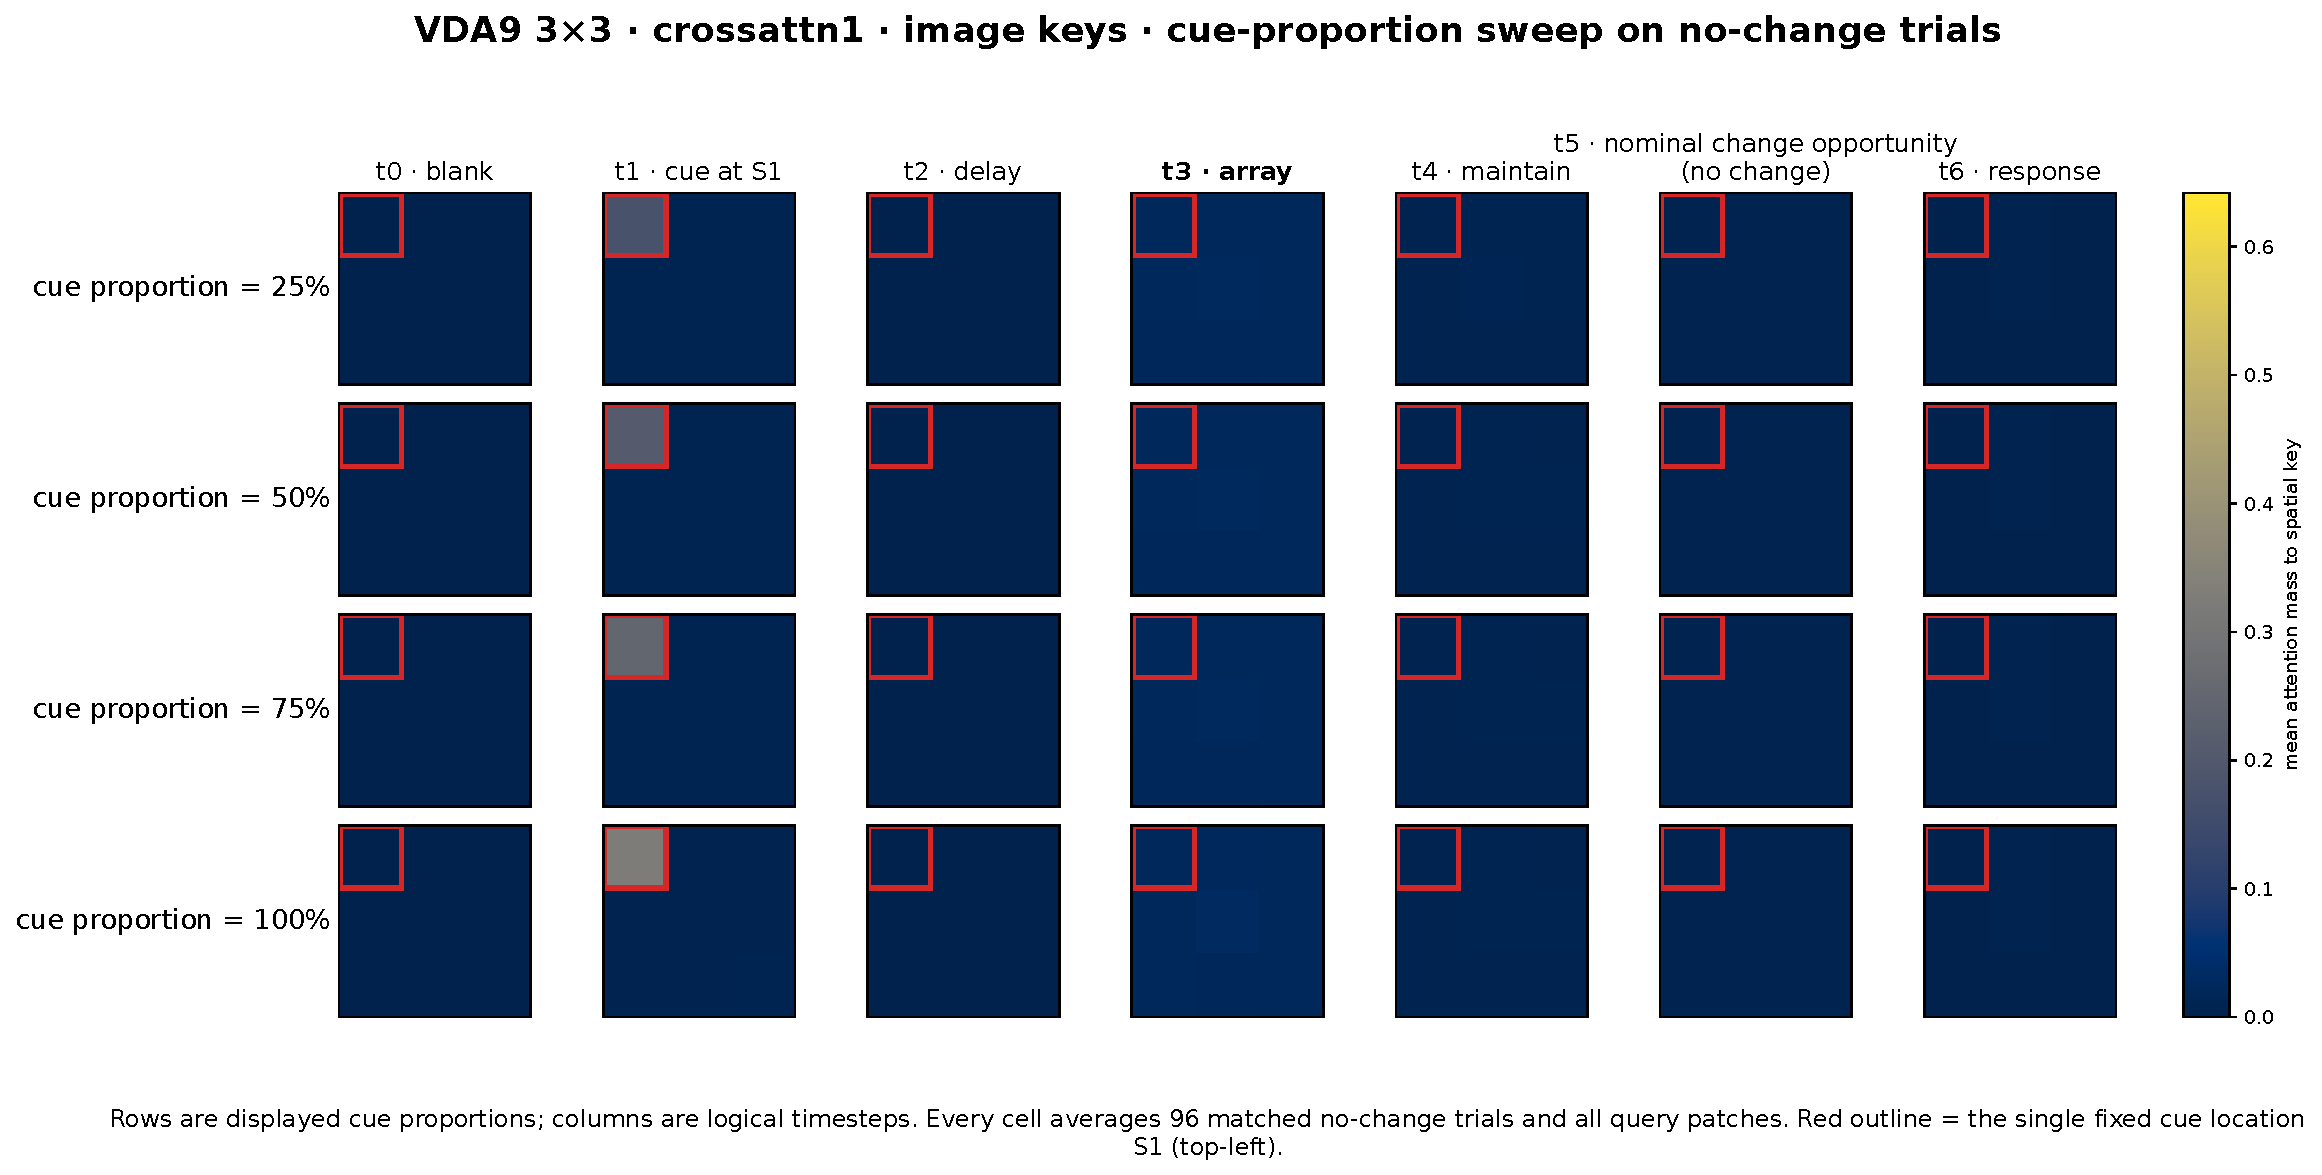
\includegraphics[width=0.96\linewidth]{first_wave_attention_vda9_crossattn1_image_keys.pdf}
\captionof{figure}{\textbf{VDA9 cross-attention to image keys on no-change trials.} \eclass{Checkpoint-recomputed descriptive measurement; 96 matched trials per displayed cue proportion.} Under uniform mass over all 18 cross-attention keys, each spatial key receives $1/18=0.0556\ldots$.}\label{fig:first-wave-attn-vda9-cross-image}
\end{center}\end{landscape}

\begin{landscape}\thispagestyle{plain}\begin{center}
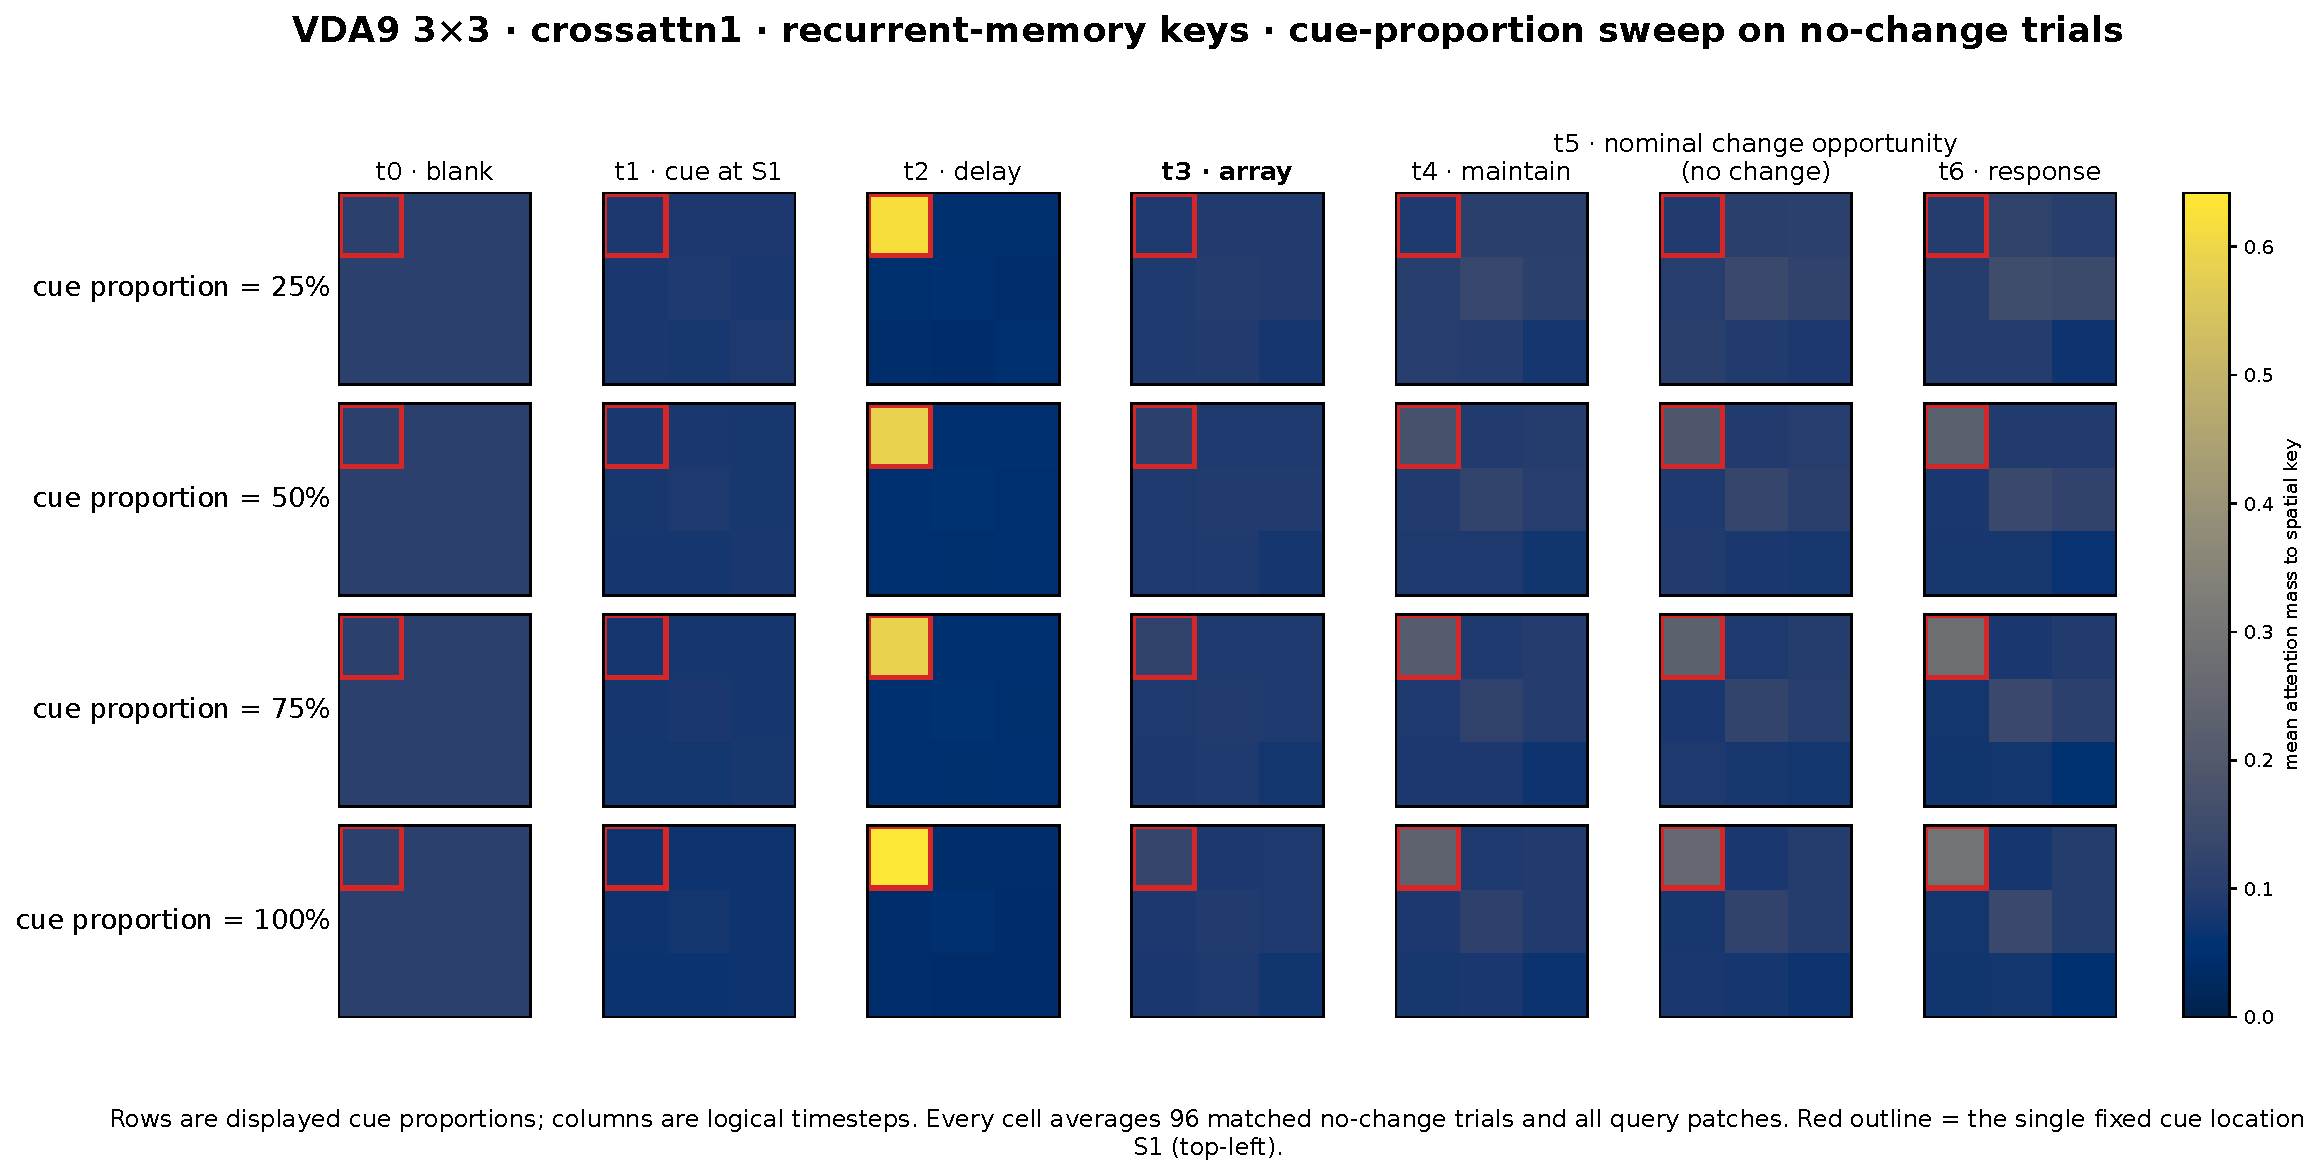
\includegraphics[width=0.96\linewidth]{first_wave_attention_vda9_crossattn1_recurrent_memory_keys.pdf}
\captionof{figure}{\textbf{VDA9 cross-attention to recurrent-memory keys on no-change trials.} \eclass{Checkpoint-recomputed descriptive measurement; 96 matched trials per displayed cue proportion.} Recurrent-memory-key $4\times7$ array, sharing scale with Figure~\ref{fig:first-wave-attn-vda9-cross-image}.}\label{fig:first-wave-attn-vda9-cross}
\end{center}\end{landscape}

\subsection{What a held-out probe can read from the recurrent state}\label{sec:width-decoding}
Each matched-width result file contains 900 trials (450 change-present, 450 no-change), four fixed folds, and reports four-fold balanced accuracy from a regularized logistic probe fitted in a common 128-dimensional space after fold-internal, train-only scaling and PCA. Change-occurrence decoding is binary over all 900 trials (chance 0.5); realized change-location decoding uses only the 450 change-present trials (VDA4 four-class, chance 0.25; VDA9 nine-class, chance $1/9\simeq0.111$); cued-vs-uncued location decoding is binary over the same 450 trials (chance 0.5). Both location targets are undefined for singleton VDA1. Timestep t0 is omitted because pre-stimulus states have zero variance and score at chance. Two native VDA9 cued-change trajectories (affine d256 and cross-attention d128) are omitted because a warning-localization process log was not retained in the upstream hash-bound evidence tree; the matched PCA-128 substitute is reported without claiming a hash-bound no-warning ledger for those two cells.

Change occurrence is strongly readable in every admitted checkpoint (t6 balanced accuracy 0.761--0.902; Table~\ref{tab:decoder-scores}). Location-conditioned readout is more variable: VDA9 affine d256 realized-location balanced accuracy is 0.499 (d128: 0.654), both well above the nine-class chance of 0.111 despite the 225/450 majority class; other defined scores reach 0.958. The corresponding d256-minus-d128 differences vary in sign -- VDA4 affine differs by 0.285 for change location, VDA4 cross-attention by $-0.050$ -- so \textbf{a wider checkpoint does not expose uniformly more linearly decodable information} in these pairs (Figure~\ref{fig:matched-width}B). These scores establish information available to the stated readout at t6; they do not establish delay maintenance, policy use, or necessity, and per Panichello and Buschman's finding that shared representational geometry requires matched attention and memory-selection tasks to demonstrate, not one task alone, we do not claim a domain-general controller from a single-task decoder \cite{panichello2021}.

\begingroup\small
\captionof{table}{\textbf{Final-timestep held-out decoder scores.} Entries are four-fold balanced accuracies at t6 in d128/d256 order; location targets are undefined for singleton VDA1.}\label{tab:decoder-scores}
\begin{tabularx}{\textwidth}{@{}p{3.0cm}p{2.2cm}Y Y Y@{}}
\toprule
Task & Routing & Change occurrence balanced accuracy d128/d256 & Change location balanced accuracy d128/d256 & Cued vs uncued balanced accuracy d128/d256\\
\midrule
VDA1 & affine & .893 / .902 & undefined & undefined\\
VDA1 & cross-attention & .897 / .888 & undefined & undefined\\
VDA4 & affine & .830 / .879 & .616 / .900 & .845 / .958\\
VDA4 & cross-attention & .818 / .833 & .842 / .792 & .936 / .907\\
VDA9 & affine & .761 / .792 & .654 / .499 & .889 / .831\\
\bottomrule
\end{tabularx}
\endgroup

\subsection{VDA16: source-resolved attention maps and readout}\label{sec:vda16-attention-dynamics}
The VDA16 attention maps use the same protocol as Section~\ref{sec:first-wave-attention}: four displayed cue proportions, 96 matched no-change trials per proportion, seven logical timesteps. Because \env{crossattn1} attends over sixteen image keys and sixteen recurrent-memory keys, uniform attention over all 32 keys would assign $1/32=0.03125$ to each. The maps show the strongest cue-localized mass in the \emph{recurrent-memory} source at t2 -- after cue presentation and before the array -- while image-key cue mass at t1 increases with displayed cue proportion (Figures~\ref{fig:vda16-attn-image}--\ref{fig:vda16-attn-memory}). The affine checkpoint exposes one sixteen-key self-attention array instead: it concentrates strongly on S1 at cue presentation and retains a weaker S1 elevation through the delay, array, nominal change opportunity, and response frames (Figure~\ref{fig:vda16-attn-affine}). A sustained, cue-directed elevation of routing mass toward a specific location during an empty delay period is the pattern Awh and Jonides's overlapping-mechanisms account predicts if spatial attention supports rehearsal of the cued location \cite{awh2001}; a routing-mass elevation during delay is not by itself evidence of rehearsal in the behavioral sense, which would require a delay-period disruption test that has not been run (Section~\ref{sec:discussion}). Foldwise decoding at VDA16's own t6 (Figures~\ref{fig:vda16-summary}B and \ref{fig:vda16-affine-summary}B) is read the same way as Section~\ref{sec:width-decoding}: it establishes change-occurrence and change-location readout at that timestep, not delay-period maintenance.

\begin{landscape}\thispagestyle{plain}\begin{center}

\includegraphics[width=0.96\linewidth]{first_wave_attention_vda16_crossattn1_image_keys.pdf}
\captionof{figure}{\textbf{VDA16 cross-attention to image keys on no-change trials.} \eclass{Checkpoint-recomputed, competence-gated descriptive measurement; 96 matched trials per displayed cue proportion.} Image-key $4\times7$ array; under uniform mass over all 32 cross-attention keys, each spatial key receives $1/32=0.03125$.}\label{fig:vda16-attn-image}
\end{center}\end{landscape}

\begin{landscape}\thispagestyle{plain}\begin{center}

\includegraphics[width=0.96\linewidth]{first_wave_attention_vda16_crossattn1_recurrent_memory_keys.pdf}
\captionof{figure}{\textbf{VDA16 cross-attention to recurrent-memory keys on no-change trials.} \eclass{Checkpoint-recomputed, competence-gated descriptive measurement; 96 matched trials per displayed cue proportion.} Recurrent-memory-key $4\times7$ array, sharing scale with Figure~\ref{fig:vda16-attn-image}.}\label{fig:vda16-attn-memory}
\end{center}\end{landscape}

\begin{landscape}\thispagestyle{plain}\begin{center}
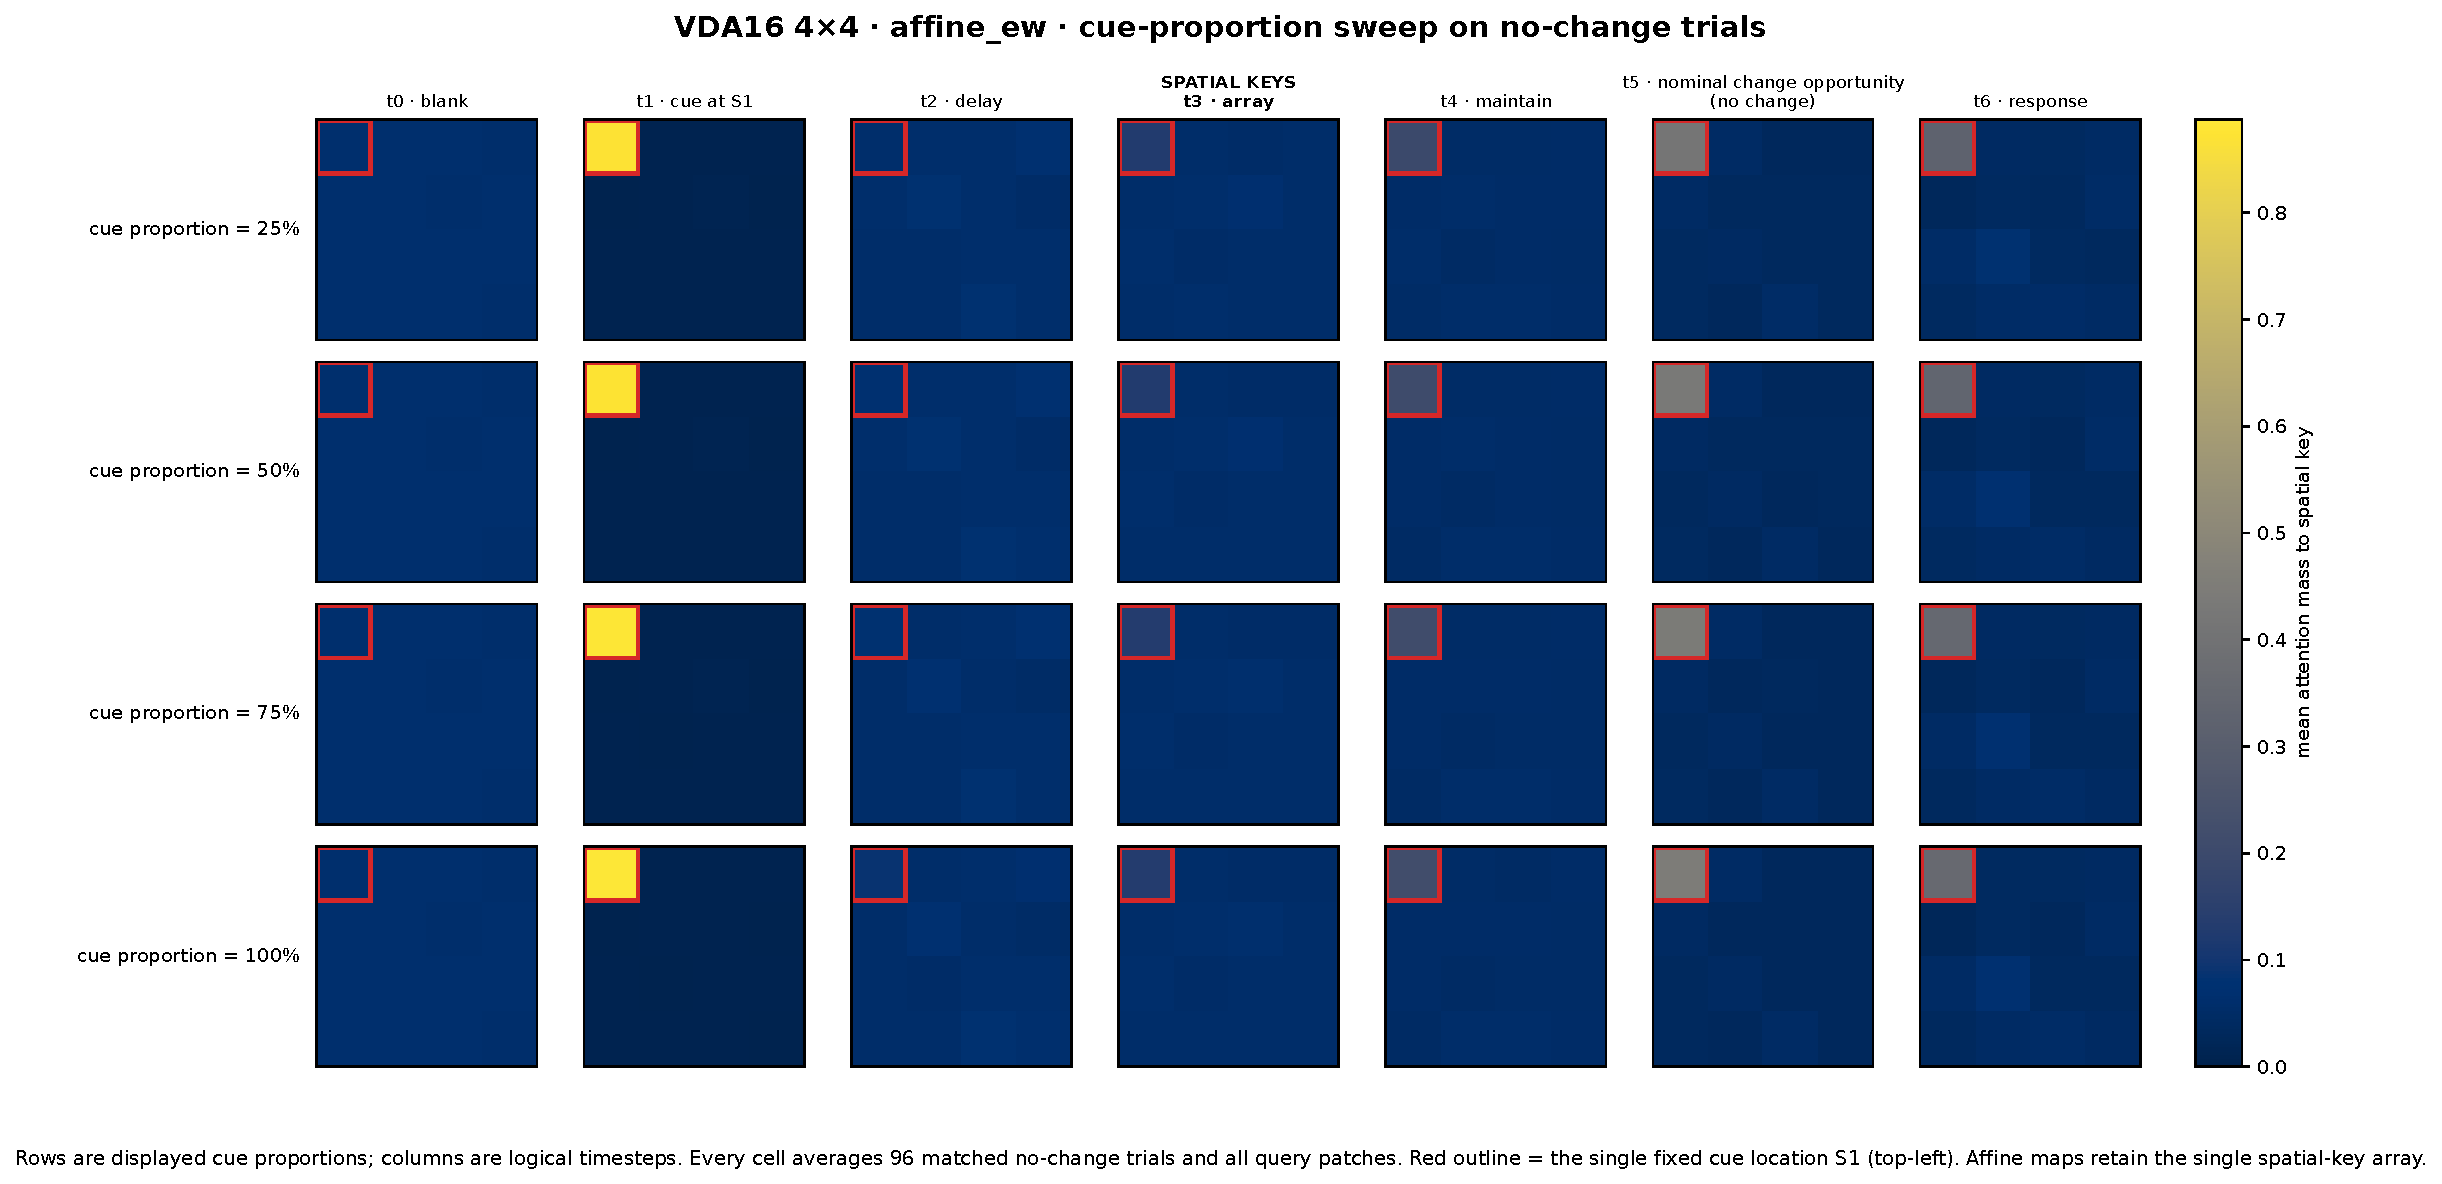
\includegraphics[width=0.96\linewidth]{first_wave_attention_vda16_affine_ew.pdf}
\captionof{figure}{\textbf{VDA16 affine self-attention on no-change trials.} \eclass{Checkpoint-recomputed, competence-gated descriptive measurement; 96 matched trials per displayed cue proportion.} Rows are displayed cue proportions and columns are logical timesteps. The single spatial-key array is the correct affine counterpart to the two source-separated cross-attention arrays above; uniform mass over sixteen keys would assign $1/16=0.0625$ to each location.}\label{fig:vda16-attn-affine}
\end{center}\end{landscape}

\subsection{Attention tracks the change location over the full timeline, more weakly when uncued}\label{sec:vda16-paired-attention}
The clearest all-timestep, valid-vs-invalid attention time course in this manuscript comes from the paired cued-vs-opposite VDA16 rerun introduced behaviorally in Section~\ref{sec:vda16-behavior}. Achieved spatial attention at a location is defined as the sum of its image-key and corresponding recurrent-memory-key mass, averaged over all sixteen query tokens; uniform allocation gives $1/16=0.0625$ per location. At the $30^\circ$ focal change on t4, before the two conditions' videos differ, mean achieved mass was 0.1477 at top-left S1 and 0.0582 at bottom-right S16 -- a paired difference of $+0.0894$ (95\% evaluation-trial interval 0.0790 to 0.0999) that is attributable only to the cue, four frames earlier. On the t5 change frame, means were 0.1022 and 0.0617, a smaller paired difference of $+0.0406$ (0.0304 to 0.0507): the physical change at S16 pulls some routing weight toward it even though it was never cued, but not as much as the cue alone had already pulled weight toward S1 (Figure~\ref{fig:vda16-cued-opposite-summary}C--D; spatial maps in Figure~\ref{fig:vda16-cued-opposite-maps}). This is the attentional counterpart of the behavioral gap in Section~\ref{sec:vda16-behavior}: the model looks less at the location that actually changes when that location was not cued, and it responds to the change there less often and later.

\begin{landscape}\thispagestyle{plain}\begin{center}

\includegraphics[width=0.84\linewidth]{vda16_cued_vs_opposite_summary.pdf}
\captionof{figure}{\textbf{VDA16 paired cued-location versus opposite-corner experiment.} \eclass{Checkpoint-rerun, competence-gated evaluation; 300 matched trials per location and magnitude.} A: qualifying change-report probability (behavioral, Section~\ref{sec:vda16-behavior}). B: conditional response timing (chronometric, Section~\ref{sec:vda16-behavior}). C: achieved attention at the changed location on t5. D: changed-location attention trajectory across all seven logical timesteps for the $30^\circ$ focal change. Attention sums the target location's image and recurrent-memory keys and averages over query tokens. Bands are 95\% evaluation-trial intervals from one checkpoint.}\label{fig:vda16-cued-opposite-summary}
\end{center}\end{landscape}

\begin{center}

\includegraphics[width=0.84\linewidth]{vda16_cued_vs_opposite_spatial_maps.pdf}
\captionof{figure}{\textbf{VDA16 achieved spatial attention at t4 and t5 for the $30^\circ$ focal change.} \eclass{Checkpoint-rerun, competence-gated evaluation.} Rows force the change at cued S1 or opposite-corner S16; columns show the pixel-matched pre-change frame and the physical-change frame. Red solid outlines mark cue S1 and green dashed outlines mark the change location. All panels share one zero-to-observed-maximum scale.}\label{fig:vda16-cued-opposite-maps}
\end{center}

\boundary{This is a within-checkpoint routing description tied to one competence-gated seed. It does not identify the internal representational mechanism, establish training-seed generality, or -- on its own -- establish that the routing difference is what causes the behavioral difference; Section~\ref{sec:intervention} is what a causal claim would require.}

\subsection{Memory decay shapes attention stability, independent of set size}\label{sec:architecture-thread}
Everything above varies task condition on a fixed architecture. A separate, architecture-level manipulation instead fixes VDA4 and varies the recurrent cell's carried-state decay rate $\lambda$ between an otherwise-matched pair of frozen checkpoints: standard ($\lambda=1.00$, no forgetting, iteration 20000) versus high-decay ($\lambda=0.80$, iteration 17949). Attention activity is measured as frame-to-frame total variation over the complete query-to-key softmax map (not total attention mass, which is fixed to 1 by the softmax normalization at every frame). The high-decay checkpoint is more active under this measure: high-minus-standard total variation is $+0.1075$ (paired trial-bootstrap 95\% interval $+0.1035$ to $+0.1115$) on affine routing, with a corresponding cross-attention decay series showing the same direction across intermediate $\lambda$ values.

Faster forgetting of the recurrent state is therefore associated with \emph{more} frame-to-frame movement in routing weight, not less: a memory that retains information longer also holds its spatial routing steadier, while a memory that decays quickly must re-derive its routing more often and does so more erratically. This connects to a body of neuroscience work in which the timescale of persistent recurrent activity is the proposed substrate for maintaining a stable spatial representation across a delay -- the same class of mechanism Luck and Vogel's capacity result and Awh and Jonides's overlapping-attention account both presuppose without directly measuring \cite{luck1997,awh2001}. Here that relationship is available as a directly manipulable, quantified architecture property rather than an assumption: within this model family, sustained attention and memory persistence are not two independent design choices but two readouts of the same recurrent decay parameter. \boundary{This is a two-checkpoint, one-seed-per-arm comparison on VDA4 only; it is evidence that decay rate and attention stability covary in this architecture, not a claim about which decay rate is ``better'' for task performance or about biological persistent-activity timescales specifically.}

\section{Attention manipulation}\label{sec:intervention}
Behavioral and attentional correspondence, however clean, cannot show that the model's routing is what \emph{causes} its behavior. The two studies this design is built to speak to made exactly that causal move: Moore and Armstrong's frontal-eye-field microstimulation retinotopically improved discrimination at the stimulated location \cite{moore2003}, and Cavanaugh and Wurtz's subcortical stimulation counteracted change blindness by restoring detection at a location the animal would otherwise have missed \cite{cavanaugh2004}. Both results depend on the intervention being spatially matched to a named location and compared against non-matching locations or conditions, not merely on ``stimulation changes performance.'' This section reports the causal-intervention evidence in this architecture: an additive bias at the \emph{cued} location (Section~\ref{sec:existing-intervention}), and the paired experiment this design was built for -- biasing the \emph{true change location} on invalid-cue trials, with cued-location and neutral-location controls (Section~\ref{sec:pending-intervention}).

\subsection{An existing lever: biasing the cued location changes sensitivity}\label{sec:existing-intervention}
Every attention module in this architecture accepts an explicit additive bias on named spatial keys before the softmax (\path{paper_encoder.py}; Section~\ref{sec:architecture}), independent of how the trial itself was generated. The matched-width and VDA16 batteries already use this to bias the \emph{cued} location's key from logical frames 5 through 6:
\begin{equation}
s'_{tqk}=s_{tqk}+b\,\mathbf{1}[t\geq5]\,\mathbf{1}[k\in\mathcal{K}_{\mathrm{cue}}], \qquad b\in\{-6,-3,0,3,6\}.
\end{equation}
For affine routing, $\mathcal{K}_{\mathrm{cue}}$ is the cued image key; for cross-attention it is the cued image key and its corresponding memory key. Each bias, condition, and checkpoint has 250 trials (matched-width) or a graded dose sweep with achieved-attention measurement (VDA16). A valid or invalid hit is a declaration at frame 5 or 6 on the corresponding change trial; a false alarm is any declaration on a no-change trial; rates are clipped to $[1/(2n),1-1/(2n)]$ before
\begin{equation}
d'=\Phi^{-1}(H)-\Phi^{-1}(F), \qquad c=-\tfrac12\left[\Phi^{-1}(H)+\Phi^{-1}(F)\right],
\end{equation}
and the plotted matched-width quantity is $D_{w,x}(b)=d'_{w,x}(b)-d'_{w,x}(0)$, with $W_x(b)=D_{256,x}(b)-D_{128,x}(b)$ comparing that effect across separately trained checkpoints. \textbf{This already establishes that the bias is response-causal}: at bias $-6$, VDA4 affine gives $D_{128,\mathrm{valid}}=-1.384$, $D_{256,\mathrm{valid}}=-0.491$ ($W_\mathrm{valid}=0.893$); VDA4 cross-attention gives $-0.544$ and $-0.736$ ($W_\mathrm{valid}=-0.192$) -- a sign reversal across checkpoints (Table~\ref{tab:clamp-constituents} behind Figure~\ref{fig:matched-width}C--D). The battery retains both $d'$ and criterion $c$ but this manuscript analyzes only $d'$ for the historical/matched-width cells; a criterion analysis is the natural companion (Section~\ref{sec:discussion}). Invalid-change effects are undefined for singleton VDA1; aggregate counts do not retain trial identities, so paired intervals are unavailable for this cell.

For VDA16, the same additive cued-key bias is swept with achieved-attention measurement recorded at every dose and condition (image-key and corresponding memory-key mass, summed and averaged over query tokens; Figure~\ref{fig:vda16-summary}C--D, Figure~\ref{fig:vda16-achieved-attention}). This measurement makes the realized intervention explicit within the checkpoint -- a nominal bias of $+6$ does not move achieved attention by a fixed, comparable amount across routing families or set sizes, so doses are comparable within a routing family, not across one.

\begin{center}

\includegraphics[width=0.82\linewidth]{vda16_clamp_achieved_attention.pdf}
\captionof{figure}{\textbf{Achieved VDA16 cross-attention cued-location attention mass under the additive bias sweep.} \eclass{Checkpoint-recomputed intervention measurement.} Image-key and corresponding recurrent-memory-key mass are summed and averaged over query tokens. Error bars describe finite evaluation trials from one checkpoint, not training-seed uncertainty.}\label{fig:vda16-achieved-attention}
\end{center}

The affine checkpoint's own sweep (Figure~\ref{fig:vda16-affine-summary}C--D, Figure~\ref{fig:vda16-affine-achieved-attention}) shows a pattern cross-attention does not: valid-trial sensitivity rises with bias, peaks, and eases back slightly ($d'=1.82$ at $b=-6$ to $2.71$ at $b=0$, peaking at $2.87$ at $b=+3$ before easing to $2.76$ at $b=+6$), but invalid-trial sensitivity falls \emph{monotonically} across the whole sweep ($d'=1.73$ at $b=-6$ down to $0.58$ at $b=+6$) even though the bias is always applied at the cued location, never at the true (uncued) change location. Criterion moves accordingly: the valid-trial criterion becomes sharply more liberal with increasing bias ($c=0.89\to0.05$) while the invalid-trial criterion stays roughly flat and, if anything, becomes slightly more conservative ($c=0.93\to1.14$). Read together with the achieved-attention curves, boosting the cued key pulls routing mass toward S1 on invalid trials too (achieved cued-location mass at t6 is 0.001 at $b=-6$, 0.134 at the natural $b=0$ baseline, and 0.796 at $b=+6$), so pushing more attention onto a location that is wrong on an invalid trial actively degrades the model's ability to detect the change elsewhere -- the same competitive logic documented directly, with the bias placed at the correct location instead, in Section~\ref{sec:pending-intervention}.

\begin{center}
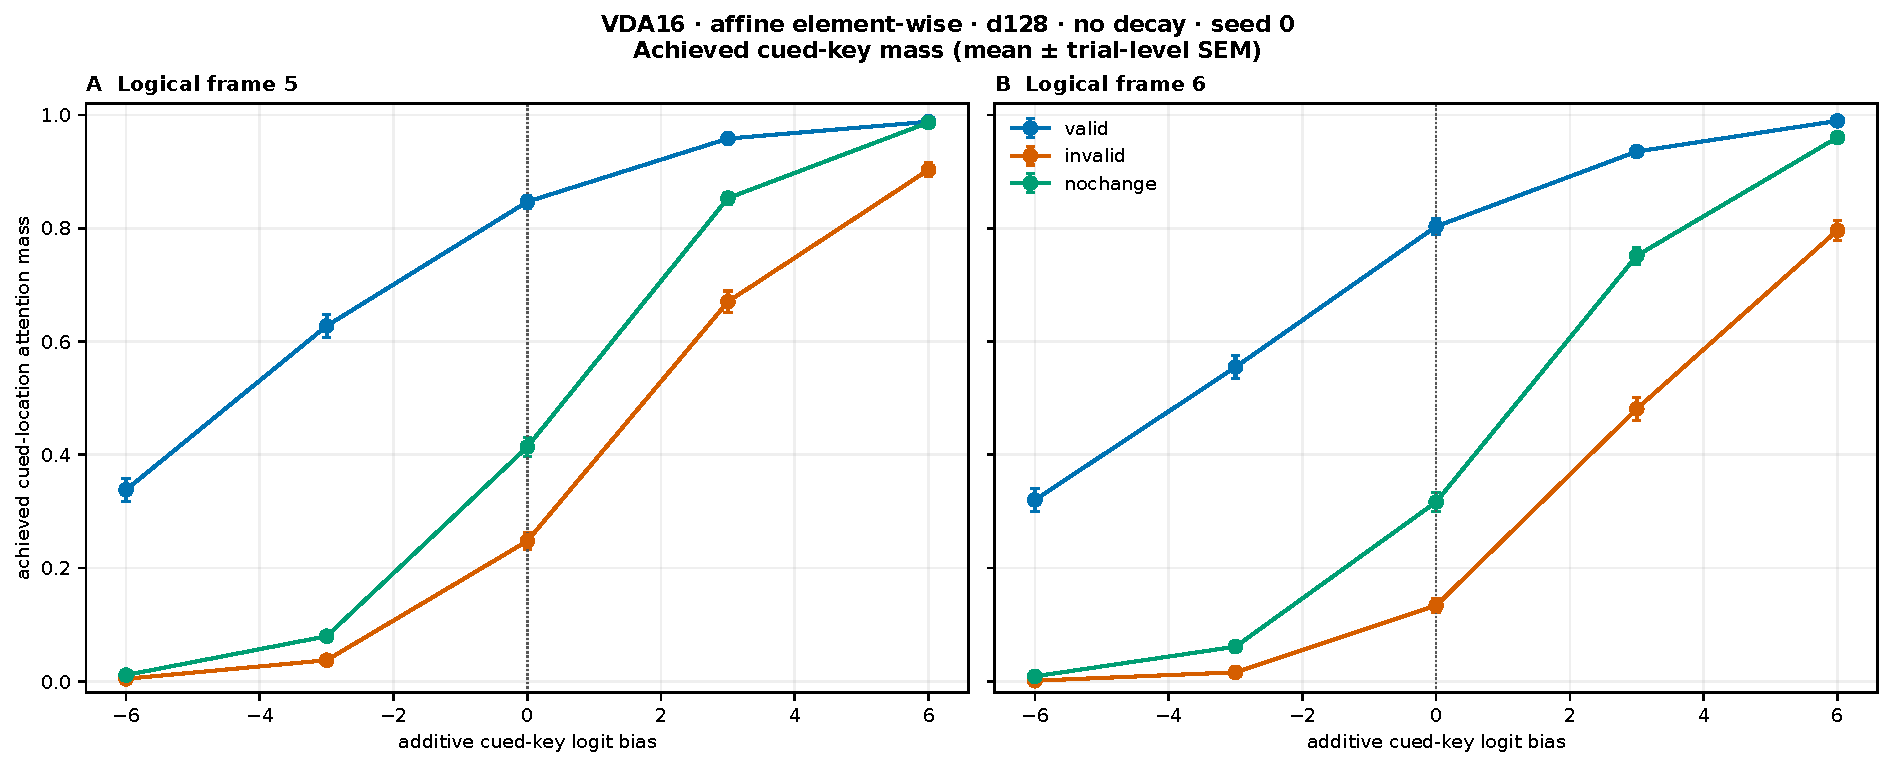
\includegraphics[width=0.82\linewidth]{vda16_affine_clamp_achieved_attention.pdf}
\captionof{figure}{\textbf{Achieved VDA16 affine cued-location attention mass under the additive bias sweep.} \eclass{Checkpoint-recomputed intervention measurement.} Self-attention key mass is averaged over query tokens. Error bars describe finite evaluation trials from one checkpoint, not training-seed uncertainty.}\label{fig:vda16-affine-achieved-attention}
\end{center}

\boundary{The existing lever establishes model-internal sensitivity to a defined routing-key bias at the \emph{cued} location, within evaluated checkpoints. It does not identify a causal width effect (Section~\ref{sec:width-behavior} already shows width itself is not consistently behavior-changing) and does not decompose the effect into sensitivity and criterion for every cell. ``Routing-key bias,'' ``clamp,'' and ``injection/inhibition'' are model-side terms; ``microstimulation analogue'' is used only with this explicit boundary attached, never as a claim of biological equivalence.}

\subsection{The rescue test: paired intervention at the true change location}\label{sec:pending-intervention}
The lever above always biases the location the cue points to, whether or not that location actually changes. Here it is instead pointed at the \emph{true change location on an invalid-cue trial} -- the one condition that directly tests the Moore--Armstrong/Cavanaugh--Wurtz logic on this model: if the routing deficit visible in Section~\ref{sec:vda16-paired-attention} (achieved attention at an uncued change location is roughly a third of the cued value even after the change occurs) is what causes the behavioral deficit in Section~\ref{sec:vda16-behavior} (qualifying response rate falling from 0.983 to 0.490 at the same focal magnitude), then restoring attention there by force should partially restore behavior, and removing it further should make an already-poor invalid trial worse still.

On trials with the change forced away from the cue (the same paired generator as Section~\ref{sec:vda16-paired-attention}, $30^\circ$ focal magnitude, 300 trials per condition, common random numbers shared across every condition below), the same graded additive key-logit bias used in Section~\ref{sec:existing-intervention} is swept independently at three locations, per trial: (1)~\emph{the true change location} -- the rescue/lesion test itself; (2)~\emph{the cued (wrong) location} -- a negative control; (3)~\emph{a third, task-irrelevant location} (S6 in the $4\times4$ grid) -- a spatial-specificity control. All three reuse the existing, already-tested primitives (graded key-logit bias, forced-location trial generation, the $d'$/criterion machinery above) rather than new model code (\path{RViT_plus_paper_jepa_grid9/analysis/change_location_intervention.py}), applied to the same admitted, hash-verified VDA16 cross-attention/d128/seed0 checkpoint used in Sections~\ref{sec:vda16-behavior}--\ref{sec:existing-intervention}.

Targeting the true change location produces the predicted double dissociation (Figure~\ref{fig:change-loc-summary}). Relative to the natural invalid-trial baseline (no clamp; qualifying response rate 0.510, $d'=1.91$), full suppression collapses response rate to \textbf{0.067} ($d'=0.38$) and full boost recovers it to \textbf{0.947} ($d'=3.33$) -- closing 92\% of the gap to the independently measured valid-trial ceiling of 0.983 (Section~\ref{sec:vda16-behavior}). Achieved attention mass at the true change location tracks this directly (Figure~\ref{fig:change-loc-summary}D, Figure~\ref{fig:change-loc-trajectory}): suppression drives it to essentially zero from the clamp onset (logical frame 5) onward, and boost drives it to 0.99 by t6, versus 0.33 at the unclamped baseline. Response timing among trials that do qualify changes little across this sweep (conditional mean frame 5.5--5.97 throughout): the intervention mainly changes \emph{whether} the model detects the change, not how quickly it responds once it does.

Neither control location reproduces the rescue. Suppressing the cued (wrong) location barely moves response rate (0.510 to 0.540); boosting it instead \emph{lowers} response rate to 0.417 and raises the no-change false-alarm rate from 0.030 to 0.247, consistent with a less stable, more trigger-happy policy rather than improved detection. Suppressing the neutral location is similarly inert (0.510 to 0.530); boosting it lowers response rate to 0.087, comparably severe to suppressing the true change location itself. Achieved attention mass at the true change location falls to 0.065 under cued-location boost and 0.034 under neutral-location boost, versus 0.334 at baseline, so the impairment from boosting the wrong location reads as competitive: forcing routing weight elsewhere pulls it away from the true change location rather than adding a generic, location-independent gain. The rescue is therefore spatially specific to the true change location, not an artifact of biasing attention anywhere.

\begin{landscape}\thispagestyle{plain}\begin{center}
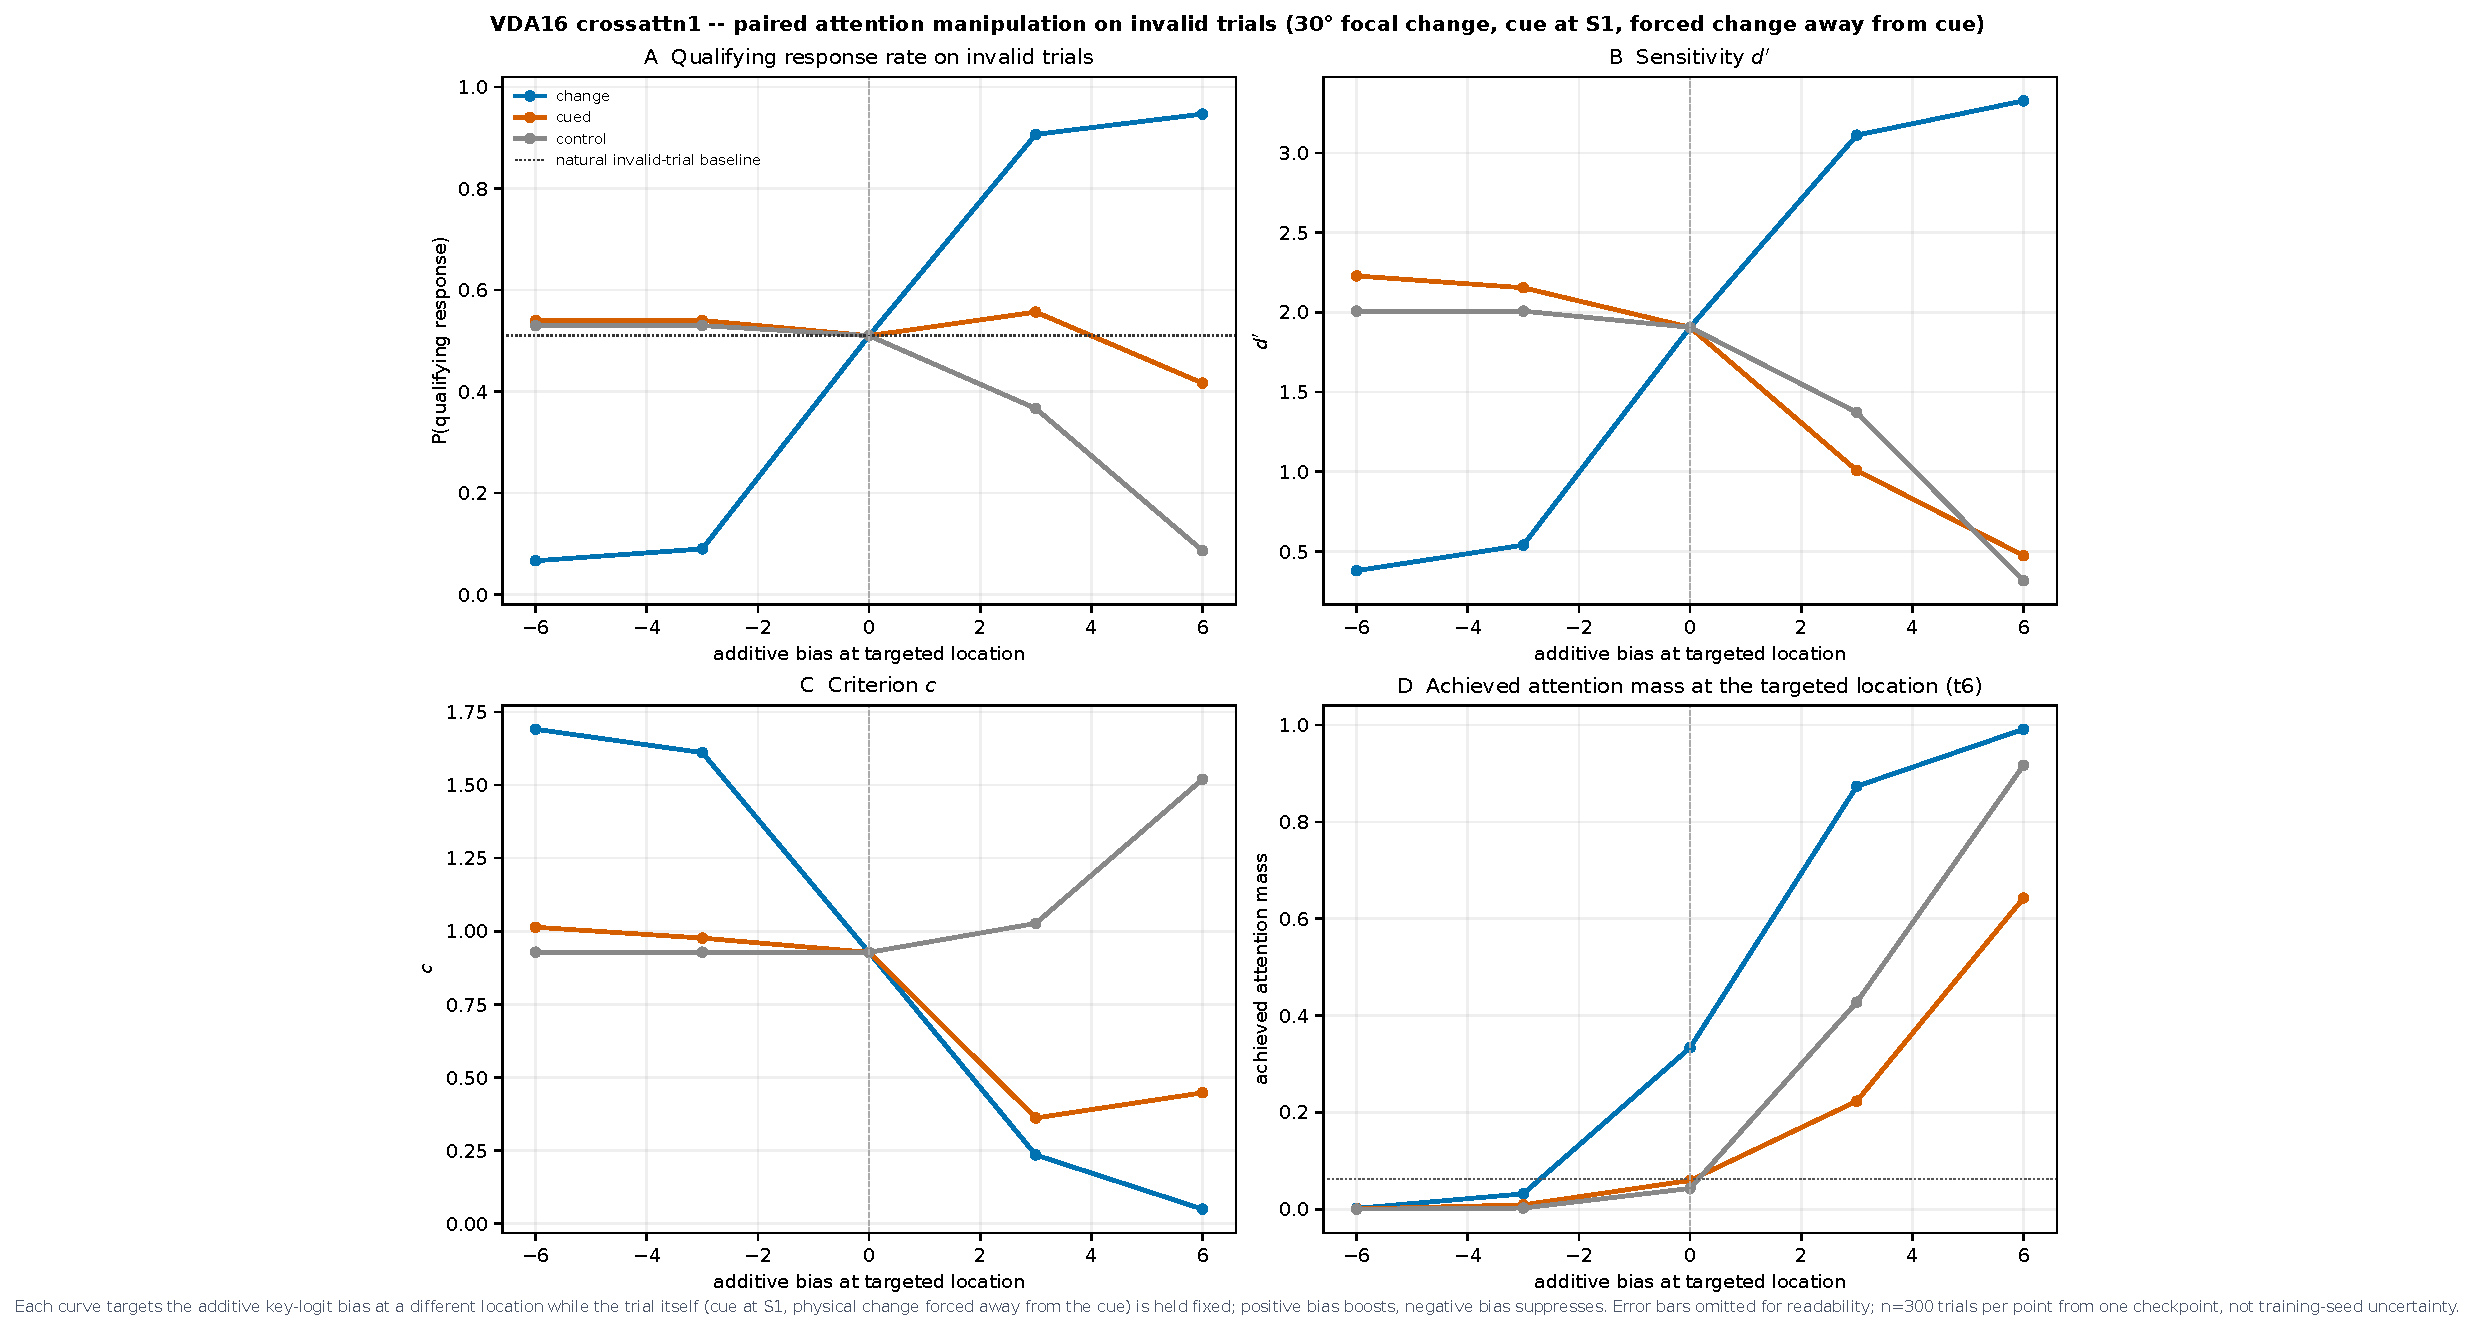
\includegraphics[width=0.86\linewidth]{vda16_change_location_intervention_summary.pdf}
\captionof{figure}{\textbf{Paired attention manipulation at the true change location, the cued location, and a neutral location, VDA16.} \eclass{Checkpoint-recomputed intervention measurement; 300 matched invalid trials per condition, one competence-gated checkpoint.} On trials with the change forced away from the cue ($30^\circ$ focal magnitude), the same graded additive key-logit bias is swept independently at the true change location, the cued (wrong) location, and a neutral control location (S6). A: qualifying response rate, with the dotted line marking the natural (unclamped) invalid-trial baseline. B: sensitivity $d'$. C: criterion $c$. D: achieved attention mass at the targeted location at t6. Only targeting the true change location rescues detection; targeting the wrong or neutral location does not, and boosting either instead lowers response rate.}\label{fig:change-loc-summary}
\end{center}\end{landscape}

\begin{center}
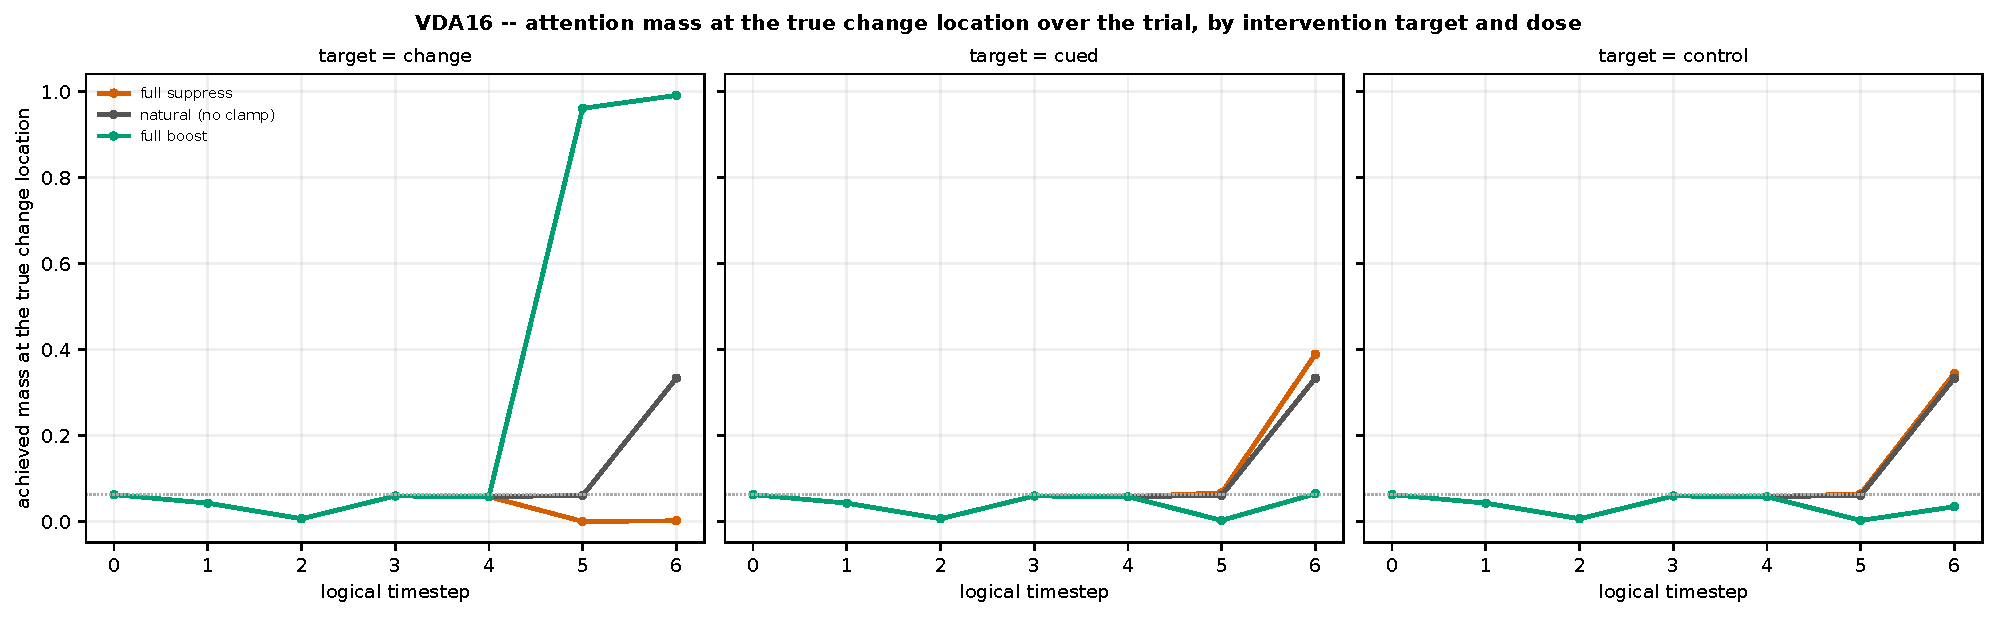
\includegraphics[width=0.92\linewidth]{vda16_change_location_attention_trajectory.pdf}
\captionof{figure}{\textbf{Achieved attention mass at the true change location across the full trial, by intervention target and dose.} \eclass{Checkpoint-recomputed intervention measurement.} Each panel targets the additive bias at a different location (change / cued / neutral); lines show full suppression, the natural unclamped condition, and full boost. The clamp is active from logical frame 5 onward. Boosting the cued or neutral location competitively reduces achieved mass at the true change location rather than leaving it at baseline; only directly targeting the true change location increases it.}\label{fig:change-loc-trajectory}
\end{center}

\boundary{This is a single-checkpoint, finite-evaluation-trial result on one competence-gated VDA16 seed. It establishes that this checkpoint's routing at the true change location is both necessary (suppression collapses detection) and sufficient (boosting it recovers detection) for its invalid-trial behavior, and that the effect is spatially specific rather than a generic gain change -- a model-level counterpart to the Moore--Armstrong/Cavanaugh--Wurtz logic, not evidence of biological equivalence. It does not establish training-seed generality, a criterion-free sensitivity account (the wrong-location conditions show criterion and false-alarm-rate changes alongside $d'$ changes), or whether the same dissociation holds at smaller set sizes.}

\subsubsection*{VDA4 and VDA9 are blocked by missing checkpoints, not by design}
The identical battery is specified for the VDA4 and VDA9 matched-width d128 checkpoints (Table~\ref{tab:width-comparison}) so that a set-size trend in the rescue effect itself, mirroring Section~\ref{sec:psychometric-fits}, could be tested. \blocked{In this working environment the checkpoint files under \path{battery_sweep_results/pod2/ckpt2/} are not present; \path{change_location_intervention.py} records this as a blocked cell per checkpoint rather than fabricating or omitting the comparison (\path{reports/vda_series/change_location_intervention_20260719/vda4/BLOCKED.json} and the \path{vda9} counterpart). Running the identical script requires no code change once those checkpoints are available.}

\section{Discussion}\label{sec:discussion}
\subsection{What is established}
The behavioral evidence, taken across the historical ladder, the checkpoint-verified first wave, the matched-width battery, and the newly admitted VDA16 checkpoints, consistently shows a cueing benefit that is present at every set size and routing family tested; whether that benefit keeps \emph{growing} with set size, however, is routing-family-specific rather than general. For cross-attention it grows monotonically to set size 16 -- a $10.9^\circ$ fitted threshold shift versus $5.3^\circ$ at set size 4, and a valid-minus-invalid response-probability gap that grows from roughly 0.2--0.3 to 0.44 across the same range (Section~\ref{sec:behavior}). The affine VDA16 checkpoint independently shows a $+0.413$ valid-minus-invalid gap at the same registered probe and stronger final-timestep decodability than its separately trained cross-attention counterpart, while advancing farther through the curriculum, but its threshold shift and raw response-probability gap both peak at set size 9 and are flat-to-falling into set size 16 (Section~\ref{sec:psychometric-fits}); those differences remain descriptive because training lineage and achieved curriculum differ. The attentional evidence shows this is not merely a labeling exercise: both VDA16 routers produce cue-localized maps, and on the cross-attention paired rerun, achieved attention at the true change location is roughly a third of its cued value at the moment of the change itself, tracking the behavioral gap (Section~\ref{sec:attention-dynamics}). A held-out probe can read change occurrence robustly and change location variably from the recurrent state at the final timestep. Recurrent memory decay rate and attention stability covary, independent of task condition (Section~\ref{sec:architecture-thread}). An additive routing-key bias at the cued location already changes model-internal sensitivity within checkpoints (Section~\ref{sec:existing-intervention}). The paired change-location test goes further: on the cross-attention VDA16 checkpoint, suppressing routing at the true change location collapses invalid-trial detection and boosting it recovers 92\% of the valid-trial gap, while the identical manipulation at the wrong cued location or a neutral location does not rescue detection and instead lowers it -- establishing that this routing is not merely correlated with behavior but spatially specific and causally load-bearing at that location (Section~\ref{sec:pending-intervention}). None of this establishes population-level precision, training-seed replication, human or primate working-memory capacity, or biological mechanism; each of those would need independent seeds, and the same battery is blocked for VDA4 and VDA9 in this environment by missing checkpoint files.

\subsection{What remains unestablished}
Three gaps matter most. First, \textbf{set size is confounded with spatial discretization} in the present design: historical VDA4/VDA9 change grid geometry and token count together with active-item count, while controlled VDA16 changes active-item count on a fixed $4\times4$ grid that itself is finer than the $2\times2$ or $3\times3$ historical grids at the same active-item count. A natural follow-up test, not run here, is to place VDA4 on the same $4\times4$ grid used by VDA16 -- i.e., \env{vda\_fixed4} rather than historical VDA4 -- and ask whether the set-size-16 cueing effect reported in Section~\ref{sec:psychometric-fits} is really about competing among more items, or about the finer spatial grid that happened to arrive together with more items in this design. \env{vda\_fixed4} is already registered (Table~\ref{tab:environments}) but its checkpoint family is currently blocked, so this comparison is future work, not a result. Second, the paired intervention in Section~\ref{sec:pending-intervention} has been run only on VDA16; the correlation between routing and behavior in Section~\ref{sec:vda16-paired-attention} is now a demonstrated causal dependency \emph{at that one checkpoint and set size}, but whether the same dissociation holds at smaller set sizes, with independent seeds, or under a criterion-controlled design remains untested -- the wrong-location conditions already show criterion and false-alarm-rate changes alongside $d'$ changes, so a full sensitivity/criterion decomposition of the rescue itself, not just the existing cued-location lever, is still needed. Third, criterion has been computed but not systematically analyzed alongside sensitivity across the whole behavioral series (Section~\ref{sec:existing-intervention} is analyzed for $d'$ only); Luo and Maunsell's central warning -- that a more liberal decision policy can raise hit rate without improving discrimination -- is only partially answered by the false-alarm check in Section~\ref{sec:psychometric-fits} and needs a full decomposition at every reported cueing effect before ``attention'' can be assigned to sensitivity, policy, or both \cite{luo2018}.

More narrowly: the aggregate historical cache carries no uncertainty or producer hash; both recomputed batteries contain one checkpoint per task--routing--width cell rather than independent training seeds; VDA16 now has terminal affine and cross-attention d128 seed-0 cells, but neither completed curriculum and no d256, decay, or independent-seed VDA16 cells exist; and two native VDA9 cued-change decoder trajectories remain excluded pending resolution of a process-log gap (Section~\ref{sec:width-decoding}). A biological citation can motivate the next test; it cannot turn a routing tensor into an anatomical structure. \boundary{The admissible language throughout this manuscript is ``model-level counterpart,'' ``structurally analogous,'' or ``corresponds to.'' No result here identifies a tensor as FEF, SC, LPFC, or biological working memory.}

\subsection{Evidence required to revise the current conclusions}
A later study could extend these conclusions only by meeting the following:
\begin{enumerate}
\item complete the remaining fixed-grid set-size families (starting with \env{vda\_fixed4}, to separate set size from spatial discretization) with matched architecture, width, budget, curriculum acceptance, and independent seeds;
\item extend the paired change-location intervention (Section~\ref{sec:pending-intervention}), currently run only on VDA16, to VDA4 and VDA9 once their checkpoint files are available, to test whether the rescue effect itself scales with set size, and add independent training seeds and a criterion-controlled design;
\item regenerate the historical behavior series with binomial intervals and separated training-seed variation;
\item extend the no-change cue-proportion routing maps to registered invalid-change and location controls, with shared scales and event alignment, at every set size;
\item extend the routing-key intervention to source-matched location controls, retained trial pairing, independent training seeds, response timing, $d'$, \emph{and} criterion together;
\item extend held-out memory and actor probes across the delay and decision path, with class semantics that separate cue-location, delay-maintenance, and change-event information, and pair any delay-period decodability with a disruption test before calling it rehearsal;
\item reserve normative VDA -- optimal sensitivity allocation under reward -- for a separate analysis rather than inferring it from empirical routing weights.
\end{enumerate}

\section{Methods and reproducibility}\label{sec:methods}
\subsection{Evidence classes and permitted conclusions}\label{sec:evidence-classes}
Every quantitative or causal claim in this manuscript is tied to an explicit evidence class. VDA means value-directed attention; M1 denotes deterministic task specification, M2 architecture documented from inspected source, M3 figures regenerated from preserved aggregate records, M4 the checkpoint-recomputed first wave, and M5 the matched-width and VDA16 intervention batteries.

\begingroup\small
\begin{tabularx}{\textwidth}{@{}p{3.5cm}p{2.7cm}Y Y@{}}
\toprule
\textbf{Evidence class} & \textbf{Current status} & \textbf{Permitted conclusion} & \textbf{Prohibited inflation}\\
\midrule
Task specification & Present (M1) & Geometry, timing, active-item count, and target-sampling semantics & Learning, convergence, capacity, or neural mechanism\\
Source-derived architecture & Present for inspected current source (M2) & Computation implemented by that source & Historical checkpoint identity, performance, necessity, or biological identity\\
Regenerated archive figure & Present from aggregate NumPy archive (NPZ; M3) & What checksum-recorded arrays display & Independent checkpoint rerun, uncertainty, or seed replication\\
Checkpoint-recomputed evaluation & VDA1, VDA4, and VDA9 at d128 and d256, plus affine and cross-attention VDA16 d128 checkpoints; three cells are competence-gated & Single-checkpoint behavior and descriptive routing under registered protocols & Population precision, training-seed replication, a common width ordering, human capacity, or biological mechanism\\
Decoder/geometry analysis & Present using foldwise train-only PCA-128 & Absolute held-out readout at a stated timestep; checkpoint-associated width contrast & Policy use, delay maintenance, necessity, causal width effect, or anatomical identity\\
Model intervention & Present as additive cued-key logit-bias clamps within admitted checkpoints, and as a paired change-location/cued-location/neutral-location intervention on VDA16 (Section~\ref{sec:pending-intervention}); the identical VDA4/VDA9 battery is blocked by missing checkpoint files & Model-internal sensitivity and SDT change under the defined dose regime; on VDA16, spatial specificity of the causal dependency at the true change location & Population-level or training-seed generality, a set-size trend in the rescue effect, or equivalence to biological microstimulation\\
Re-analysis (logistic fit) & Present over already-cached first-wave/VDA16 psychometric arrays (Section~\ref{sec:psychometric-fits}) & Threshold/slope summaries of already-verified response-probability data & A new checkpoint result; population-level threshold estimate\\
Controlled multi-seed series & Incomplete; terminal VDA16 affine and cross-attention d128 seed-0 cells are admitted, but no independent seeds exist and neither completed curriculum & Descriptive evidence from each admitted checkpoint under its frozen protocol & Capacity, curriculum completion, population convergence, or a causal routing-family effect from separately trained competence-gated cells\\
\bottomrule
\end{tabularx}
\endgroup

Coverage status and epistemic claim support are separate axes. A cell is publication-coverage \emph{complete} only when its estimand is defined, the admitted evidence and publication exports exist, the manuscript places or explicitly accounts for the product, and rendered-page QA passes; this does not establish historical producer or checkpoint identity. \emph{Partial} denotes related but incomplete evidence. \emph{Available} means a corrected producer can be run against apparently suitable evidence. \emph{Training} is reserved for an unfinished prospective checkpoint. \emph{Blocked} identifies a missing or inadmissible prerequisite. \emph{Undefined} means the estimand does not exist in the environment. \emph{Inapplicable} means the source comparison lies outside the admitted scientific scope. \emph{Blocked} additionally covers the VDA4/VDA9 arms of the change-location intervention in Section~\ref{sec:pending-intervention}: the design is specified and the reused primitives are already tested, but the checkpoint files are not present in this working environment.

\subsection{Source and figure workflow}\label{sec:source-workflow}
The MAH PDF and source archive were preserved unchanged. Active \verb|includegraphics| parsing identified five main-text and seventeen supplementary image objects; captions and included images were inspected to define 68 coherent panel groups mapped to the fourteen registered environments in Table~\ref{tab:environments}. Deterministic M1 schematics read task specifications. M2 reads architecture specifications traced to inspected current source; it is not evidence of historical checkpoint source identity. M3 reads the archived NPZ only, importing neither the training stack nor a model. The first wave executes exact selected checkpoints after freezing source bytes, writes trial-level and reduced NPZ arrays before plotting, and validates cache semantics and hashes against immutable retained bytes. The matched-width producer separately publishes twelve checkpoint-bound result files and a 34-file immutable upstream tree; its independent scientific artifact review returned \textsc{Approve with limits} (numerical reconstruction passed; separate-checkpoint, finite-trial, decoder-warning, competence-gate, and non-equivalent cross-routing intervention limits remain active). Each VDA16 producer admits one terminal checkpoint against its embedded task, routing, width, geometry, iteration, metrics, producer hashes, and checkpoint digest, then writes deterministic psychometric, decoder, timing, clamp, achieved-attention, and source-resolved attention caches under a validation gate. The affine bundle additionally freezes the already-admitted cross-attention shard before rendering the paired routing-family context figure. The logistic-fit re-analysis (Section~\ref{sec:psychometric-fits}) is produced by \path{RViT_plus_paper_jepa_grid9/analysis/psychometric_fits.py}, which loads only the already-hashed first-wave and VDA16 psychometric NPZ caches, records each source file's own SHA-256 alongside every fitted parameter, and performs no checkpoint or Torch access.

\subsection{Quality control}
Figure code was developed under focused regression tests; the current repository suite (266 tests, including 113 focused first-wave and attention-correctness tests) covers cache and checkpoint identity, exact inventory, no-change trial semantics, matched stimulus generation, cue-proportion rows, source-separated cross-attention arrays, target-specific decoder support and chance levels, sample-size conservation, undefined decoder estimands, competence gating, and read-only audit regressions. The VDA16 production shard separately passed checkpoint admission, contiguous-metrics, matched-protocol, deterministic-cache, achieved-attention, source-graph, and frozen-input validation. The manuscript was compiled with a XeTeX-compatible engine, diagnostics were scanned for overfull boxes, missing glyphs, and undefined references, and every final PDF page was rendered and inspected.

\section{Conclusion}
A recurrent vision transformer trained on cued visual change detection shows the behavioral, attentional, and (at the cued location) causal signatures of spatial cueing at every set size and routing family tested. In the cross-attention lineage all three sharpen as set size grows from 4 to 16 -- a bigger competing set is what makes the cueing effect dramatic there, both in response probability and in fitted psychometric threshold -- but the affine lineage's cueing benefit peaks at set size 9 and does not grow further into set size 16, so a bigger competing set is not by itself a sufficient explanation: which routing family is asked matters at least as much as how many items compete. Routing weight tracks the cue during the delay and tracks the true change location more weakly when that location was never cued, in a pattern that lines up with the behavioral cost of an invalid cue. An existing routing-key intervention shows this circuitry is not epiphenomenal at the cued location. The specific test this design was built for goes further: on the VDA16 checkpoint, suppressing attention at the \emph{true} change location on an invalid trial collapses detection, and boosting it there recovers 92\% of the valid-trial gap, while the identical manipulation at the wrong cued location or a neutral location does not rescue detection and instead lowers it -- a spatially specific double dissociation that is the model-level counterpart of the Moore--Armstrong microstimulation and Cavanaugh--Wurtz change-blindness logic this paper opened with. The same battery is specified for VDA4 and VDA9, to ask whether the rescue effect itself scales with set size, and is blocked in this environment only by missing checkpoint files, not by design. A second, narrower finding is architectural rather than task-driven: recurrent memory decay rate and moment-to-moment attention stability covary in this model family, independent of task condition. Neither finding licenses a claim about human or primate capacity, and neither routing tensor is a claim about a specific brain region; both are stated as model-level counterparts to a real, cited experimental tradition, with the boundary of that correspondence given beside each claim rather than collected at the end.

\clearpage
\appendix
\begin{landscape}\thispagestyle{plain}
\section{Fourteen-environment task atlas}
Figure~\ref{fig:m1-atlas} is an overview of all deterministic M1 task products. It is intended for cross-environment comparison; the companion directory contains a full-resolution vector PDF and metadata record for every environment.
\begin{center}
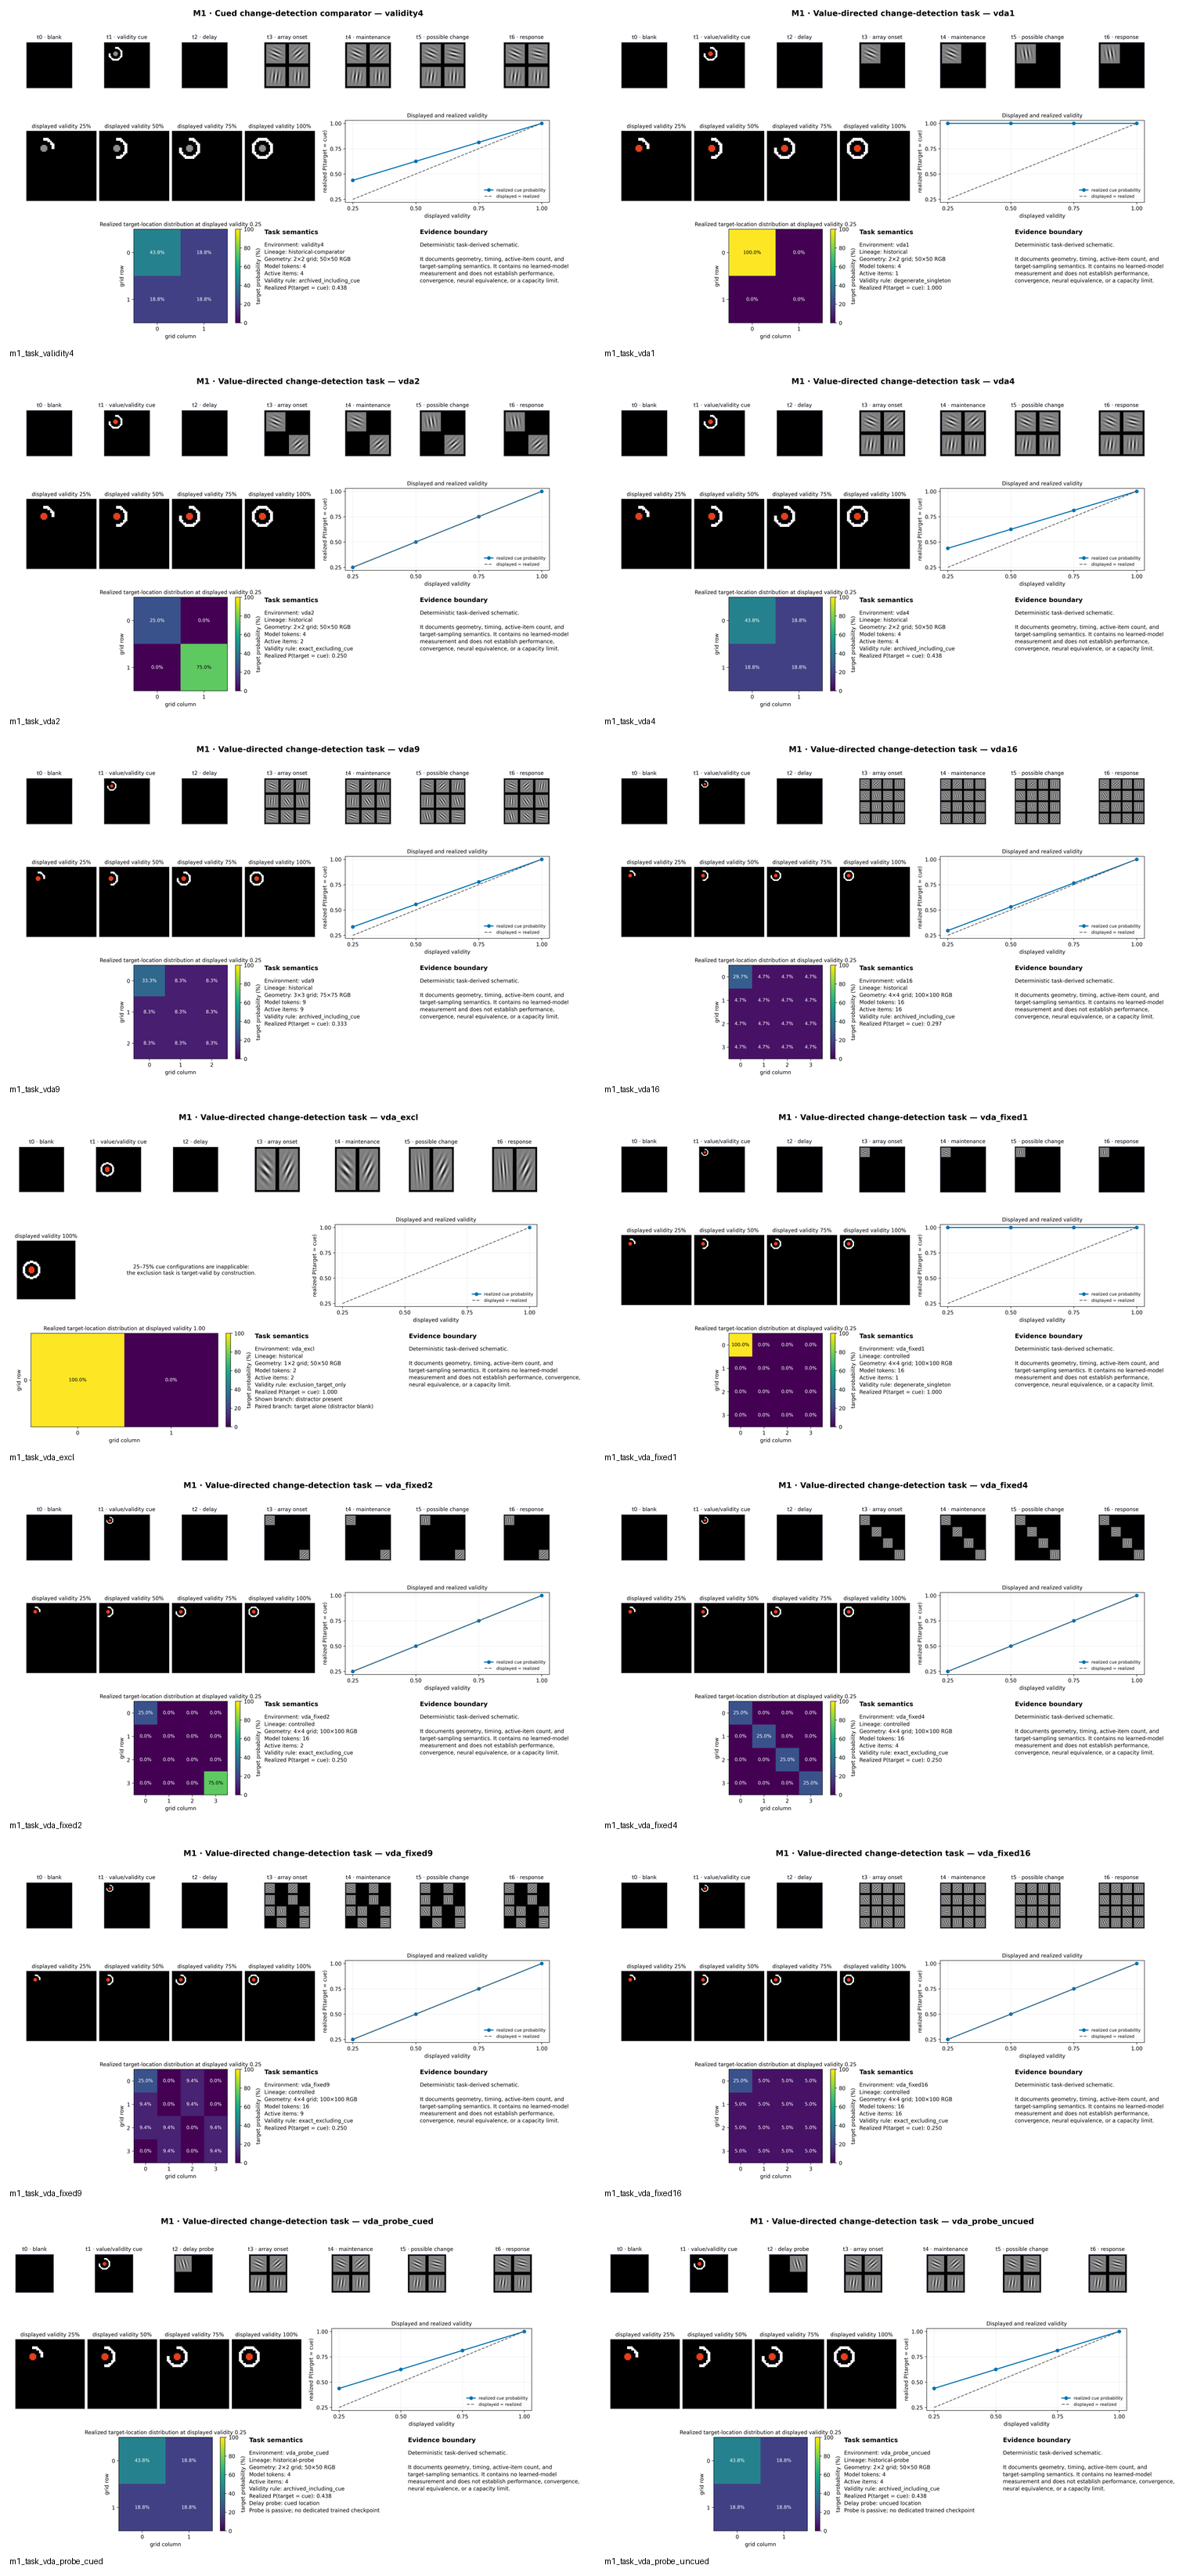
\includegraphics[height=0.68\textheight]{m1_task_contact_sheet.png}
\captionof{figure}{\textbf{M1 task atlas.} \eclass{Deterministic task-derived schematics.} Reading left-to-right and top-to-bottom, tiles show the neutral-validity comparator; historical VDA1/2/4/9/16; the exclusion task; cued and uncued delay probes; and controlled fixed-grid VDA1/2/4/9/16. Every tile uses the same seven-frame sequence, geometry/active-item display, realized-target heatmap, and task-semantics block.}\label{fig:m1-atlas}
\end{center}\end{landscape}

\newcommand{\MThreeFullPlates}{%
\begin{landscape}\thispagestyle{plain}
\section{Full historical aggregate plates}\label{app:m3-full}
\begin{center}
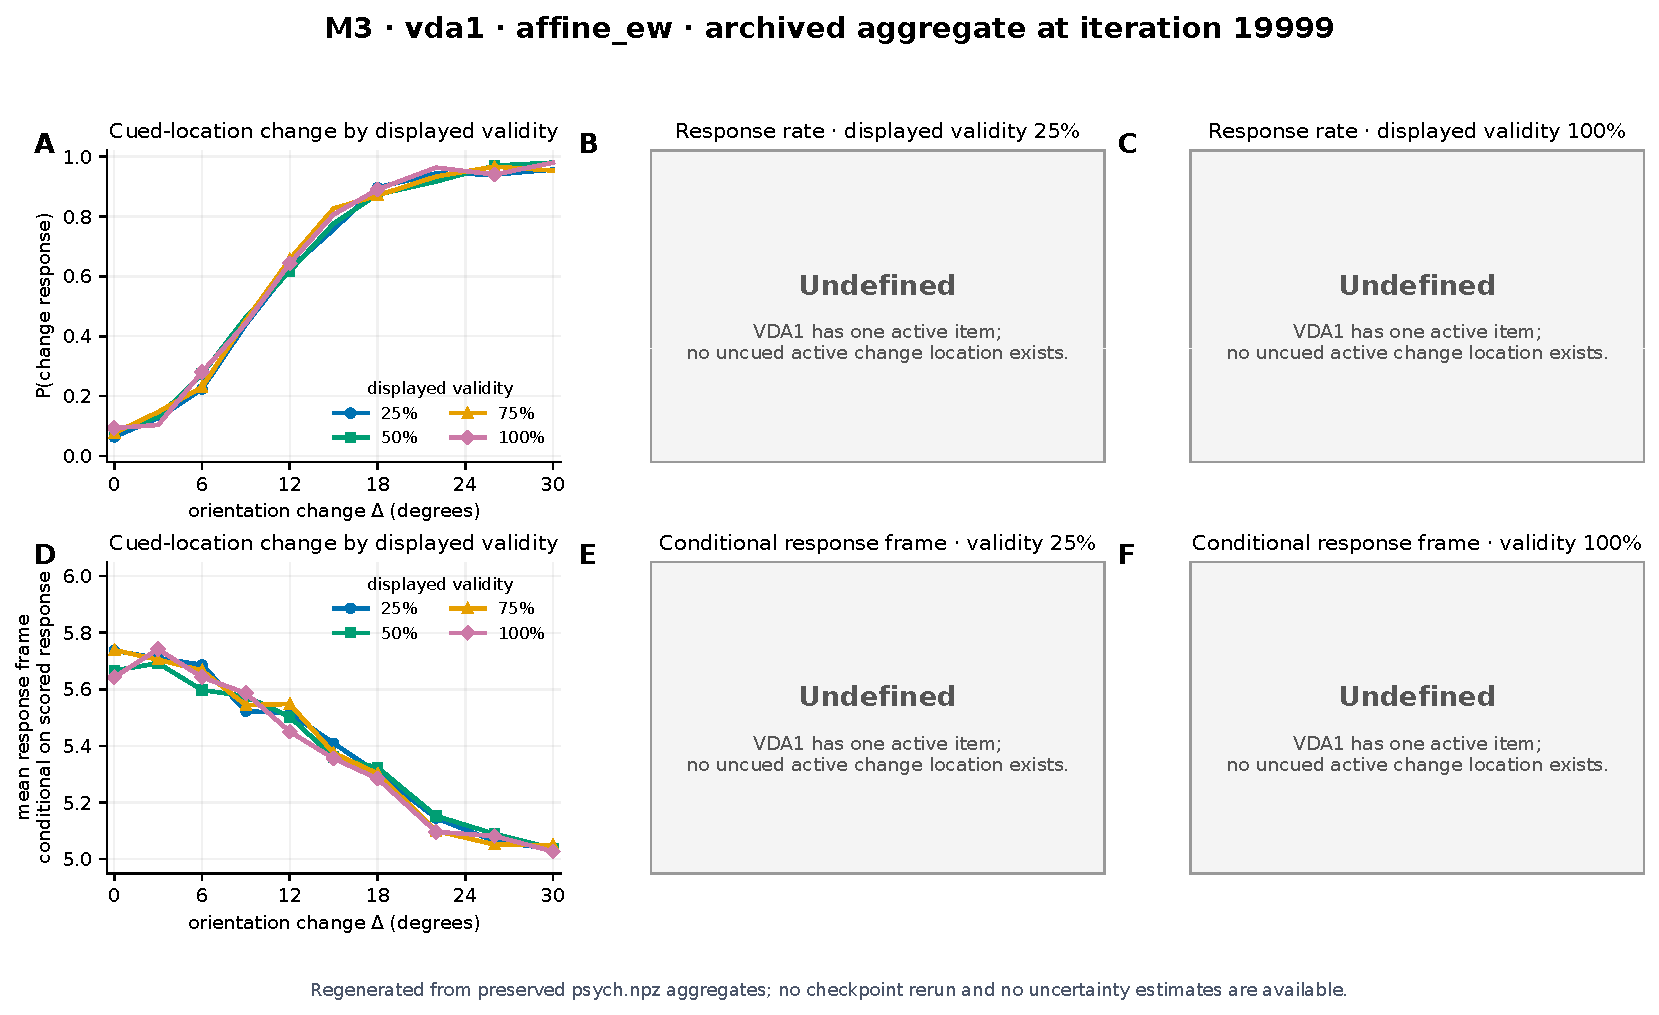
\includegraphics[width=0.89\linewidth]{m3_behavior_vda1_affine_ew.pdf}
\captionof{figure}{\textbf{Historical VDA1, affine feedback.} \eclass{Regenerated from preserved aggregate NPZ; checkpoint not rerun.} Change-response probability generally rises and conditional mean response frame falls with change magnitude. The singleton task defines only cued-location panels A and D; uncued-location panels B, C, E, and F are scientifically undefined.}\label{fig:m3-vda1-affine}
\end{center}\end{landscape}

\begin{landscape}\thispagestyle{plain}\begin{center}
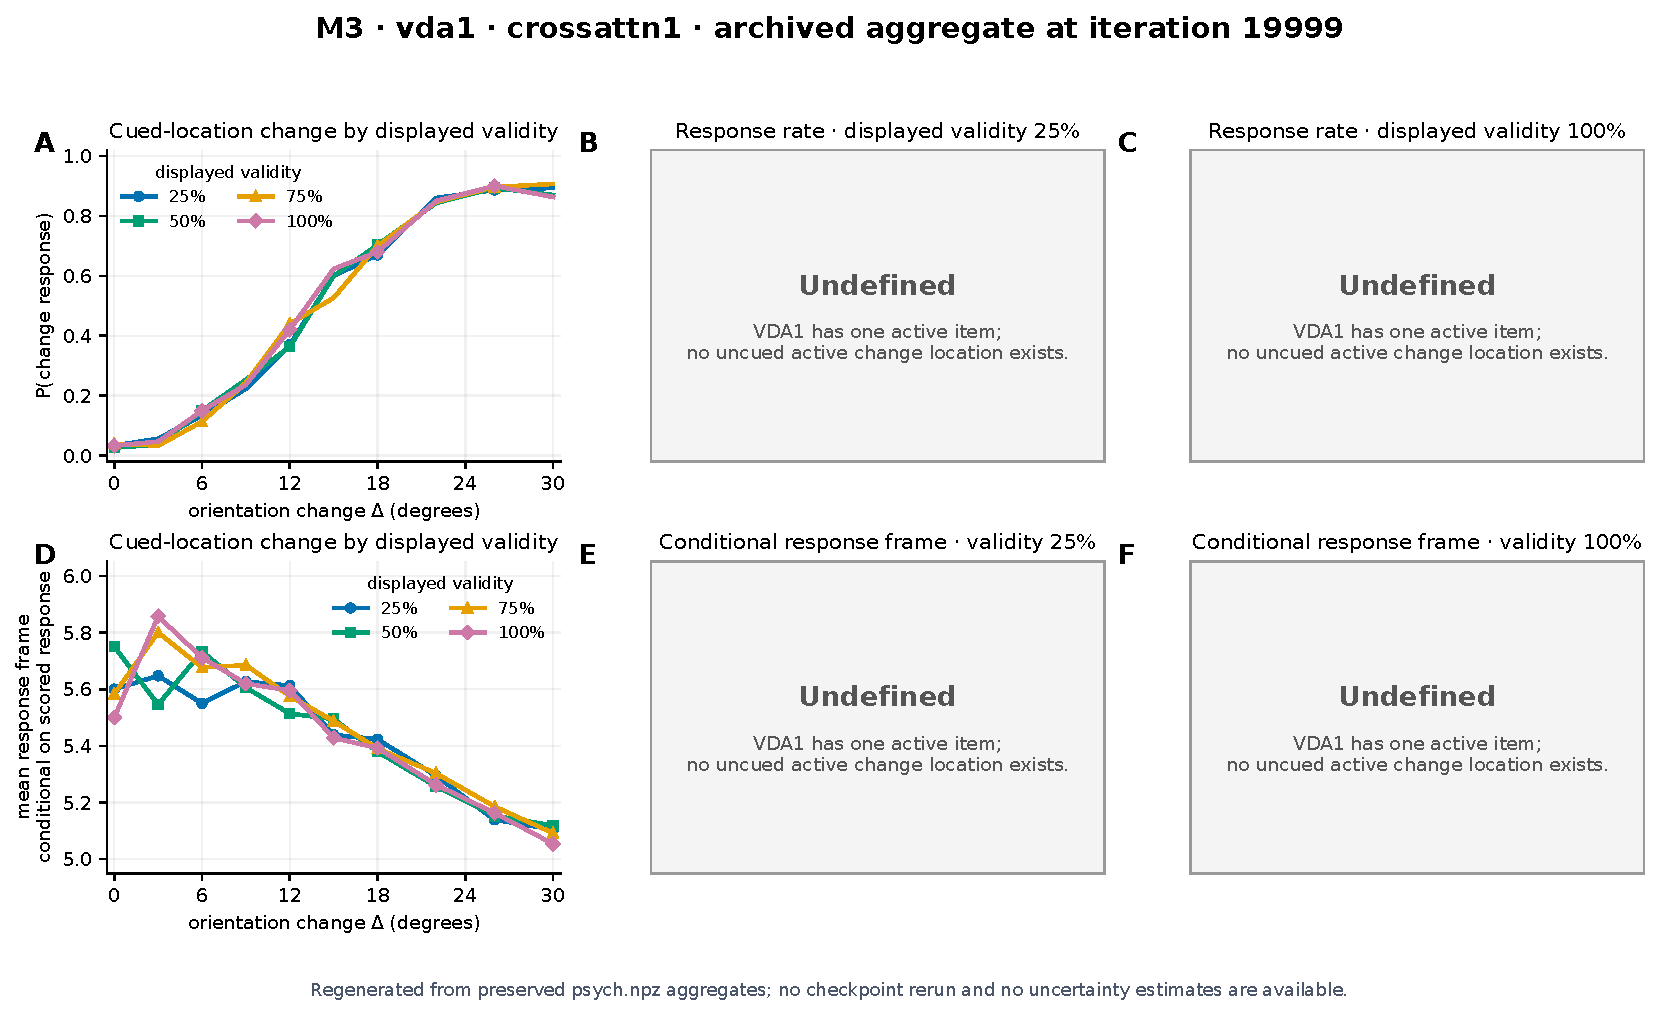
\includegraphics[width=0.89\linewidth]{m3_behavior_vda1_crossattn1.pdf}
\captionof{figure}{\textbf{Historical VDA1, cross-attention.} \eclass{Regenerated from preserved aggregate NPZ; checkpoint not rerun.} No uncued active location exists; these are cache entries, not an independently verified checkpoint execution.}\label{fig:m3-vda1-cross}
\end{center}\end{landscape}

\begin{landscape}\thispagestyle{plain}\begin{center}
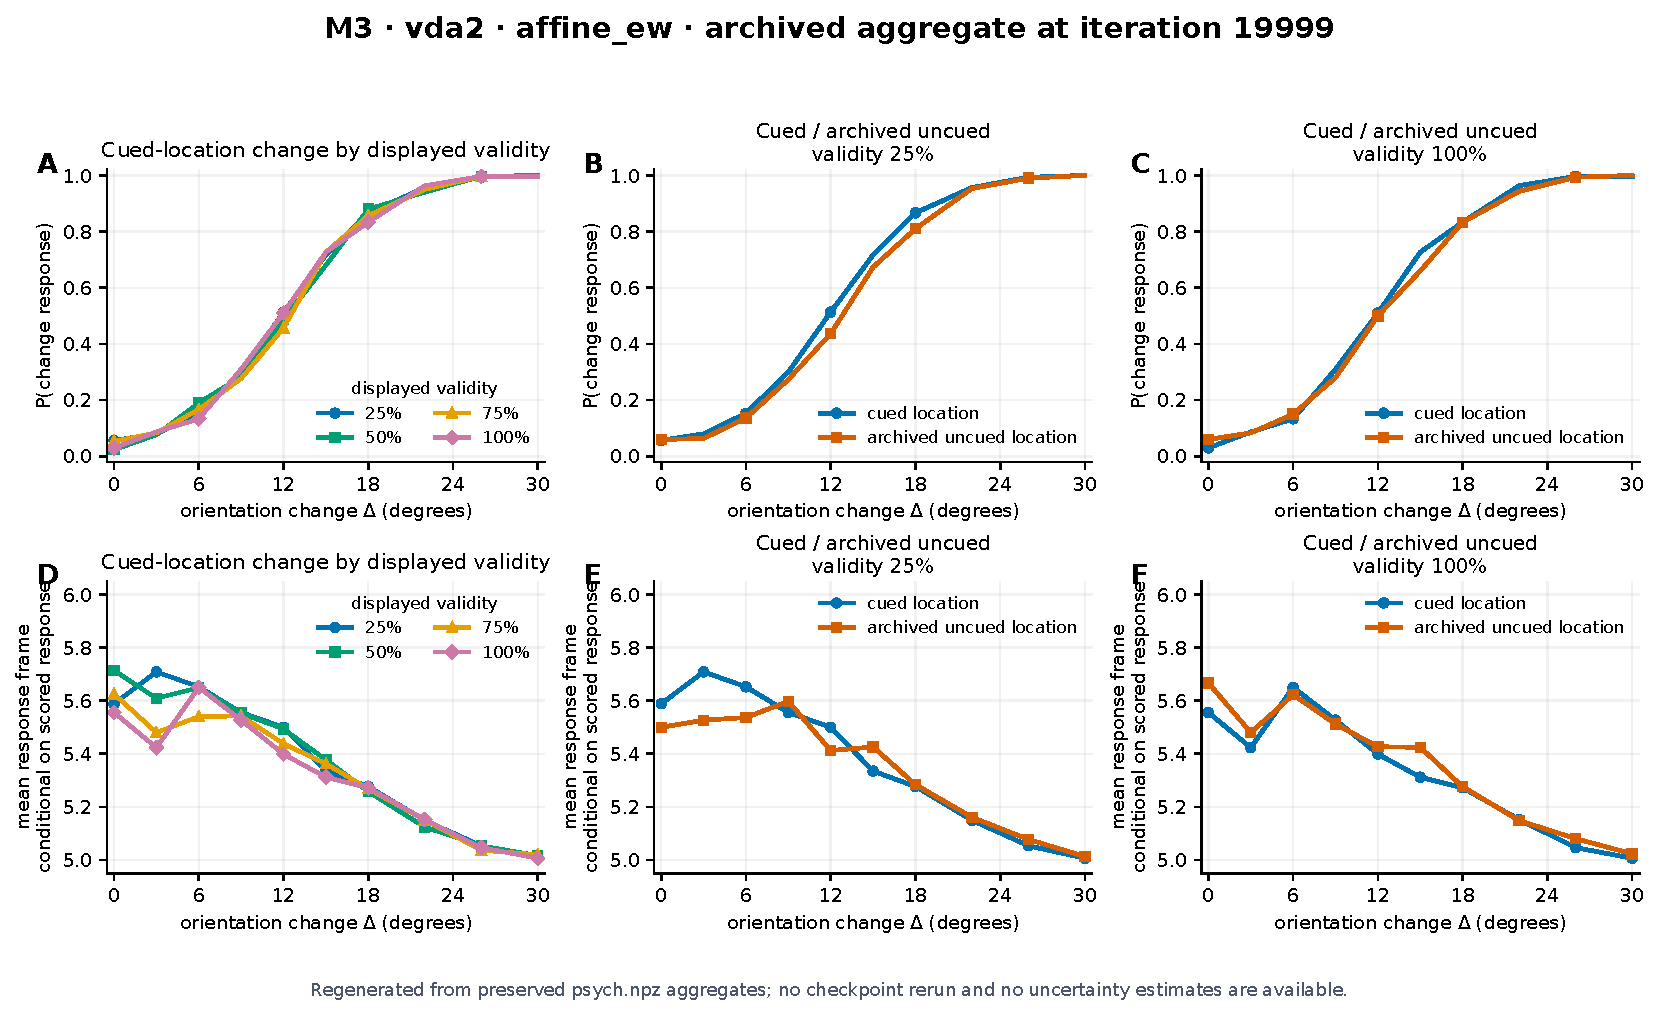
\includegraphics[width=0.89\linewidth]{m3_behavior_vda2_affine_ew.pdf}
\captionof{figure}{\textbf{Historical VDA2, affine feedback.} \eclass{Regenerated from preserved aggregate NPZ; checkpoint not rerun.} Cued and archived uncued curves are mostly close; the NPZ does not prove the uncued spatial index.}\label{fig:m3-vda2-affine}
\end{center}\end{landscape}

\begin{landscape}\thispagestyle{plain}\begin{center}
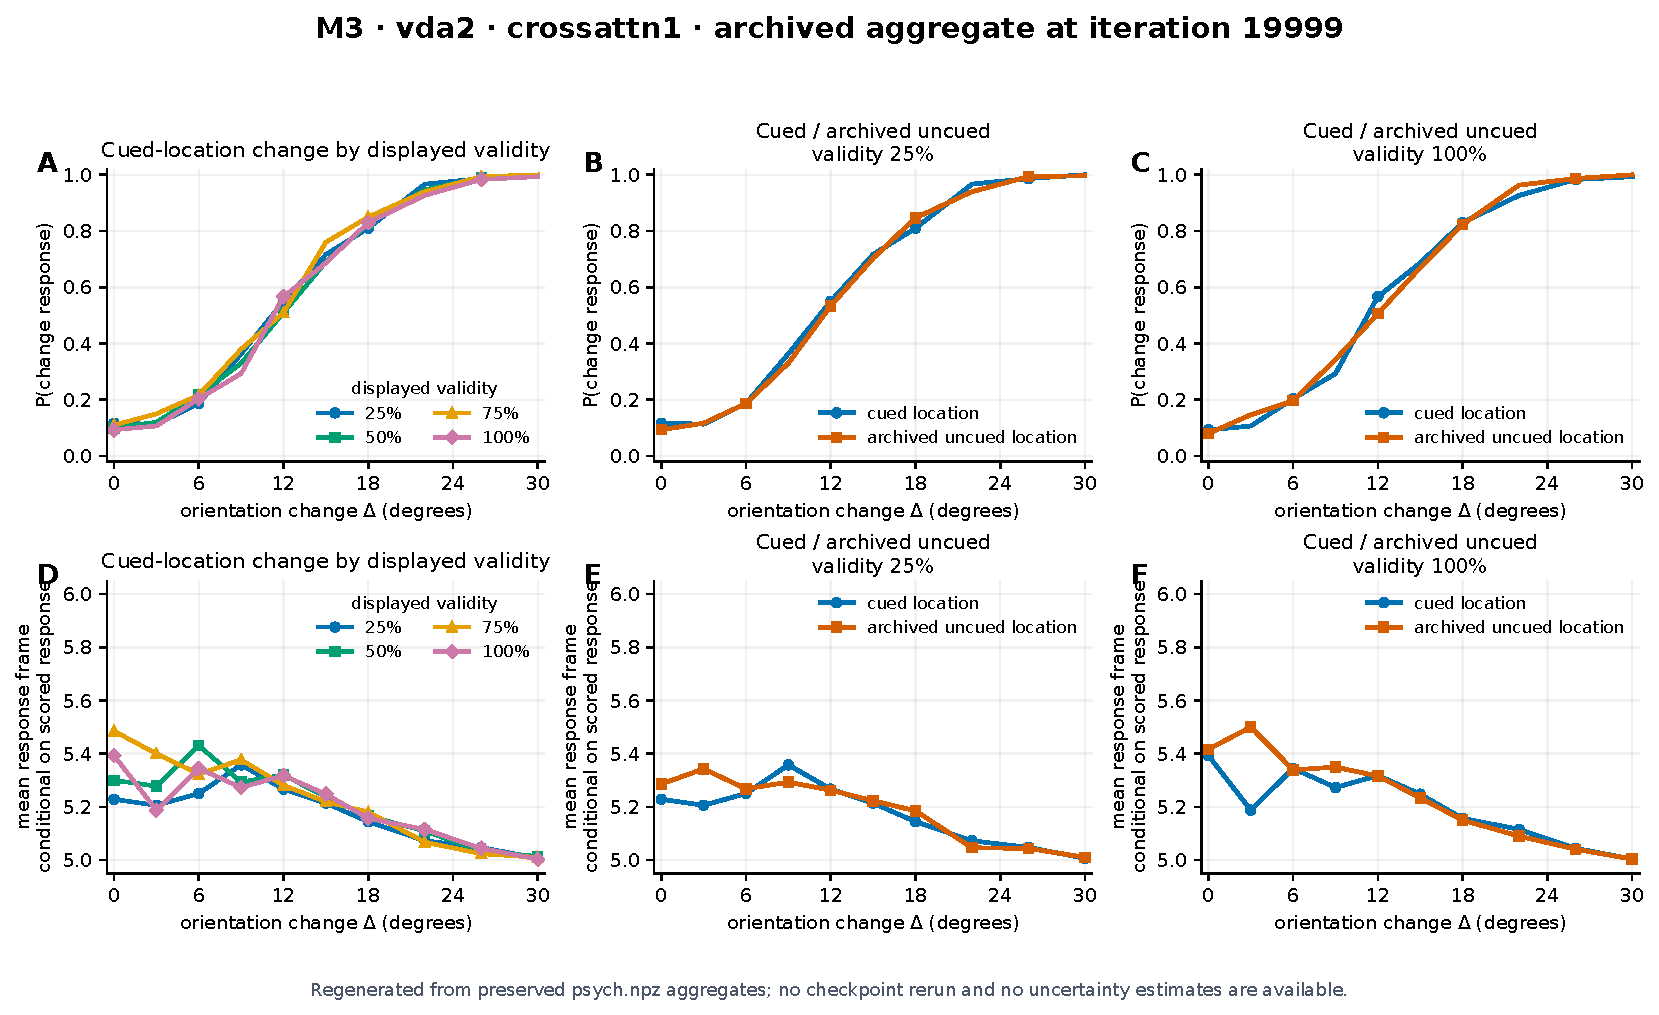
\includegraphics[width=0.89\linewidth]{m3_behavior_vda2_crossattn1.pdf}
\captionof{figure}{\textbf{Historical VDA2, cross-attention.} \eclass{Regenerated from preserved aggregate NPZ; checkpoint not rerun.} Cued and archived uncued point-estimate curves are mostly close, without uncertainty or seed replication.}\label{fig:m3-vda2-cross}
\end{center}\end{landscape}

\begin{landscape}\thispagestyle{plain}\begin{center}
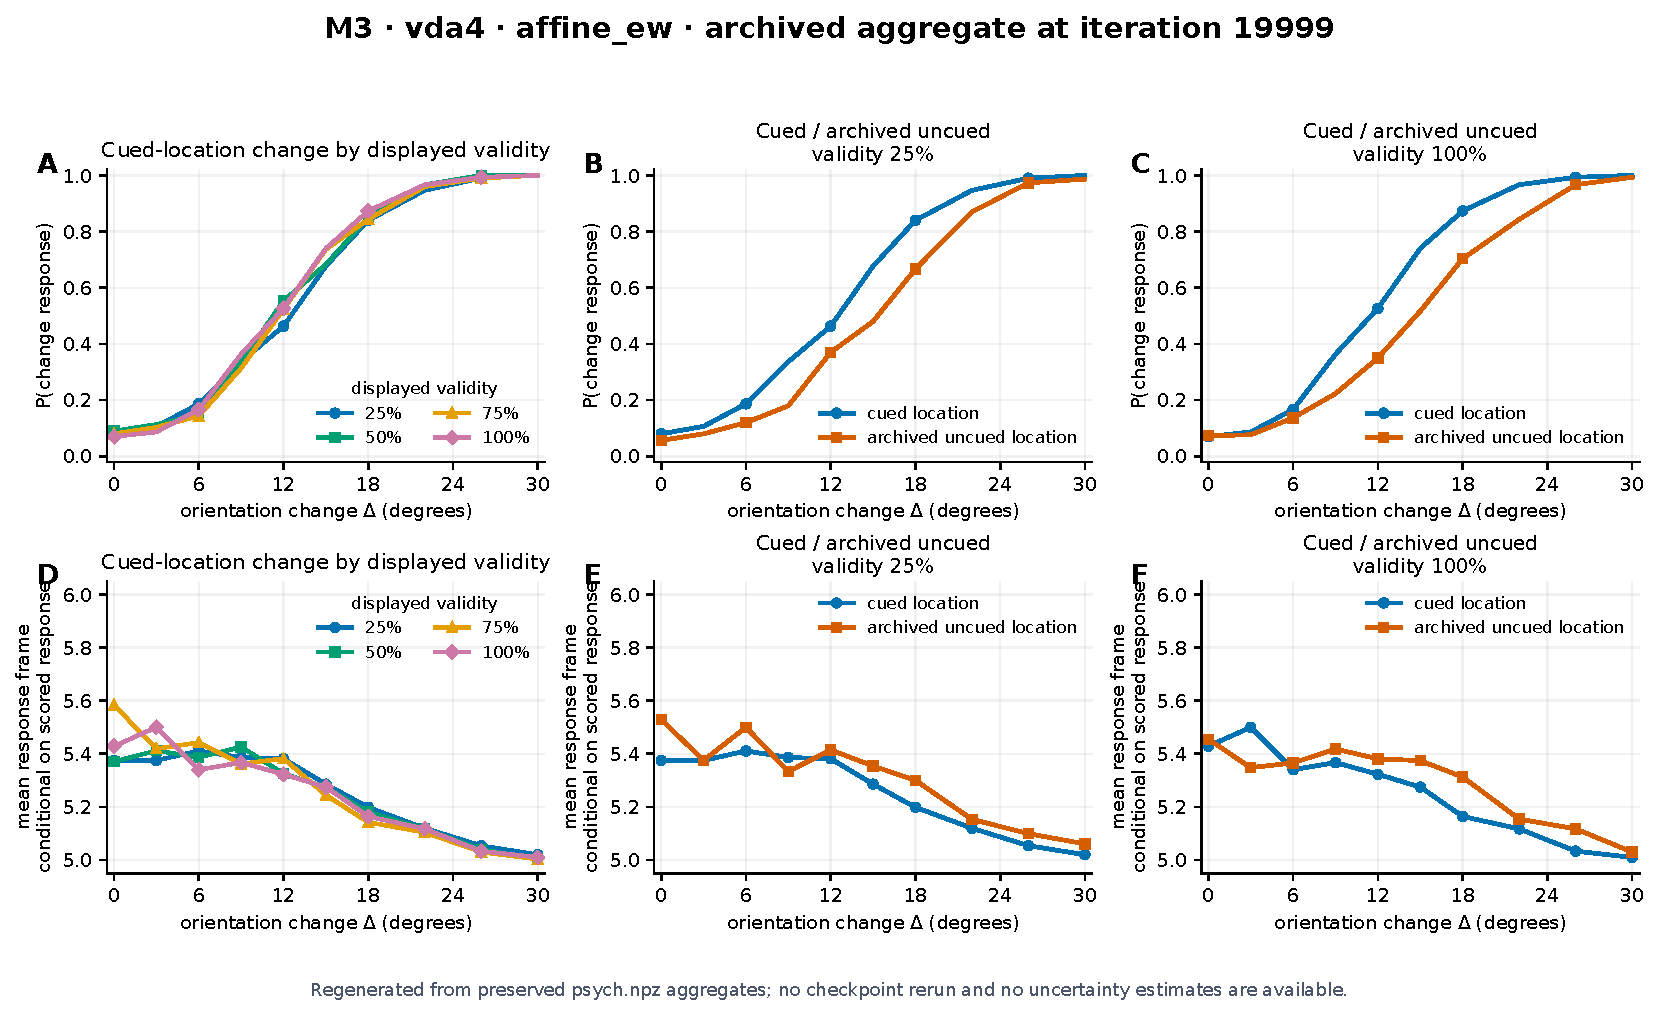
\includegraphics[width=0.89\linewidth]{m3_behavior_vda4_affine_ew.pdf}
\captionof{figure}{\textbf{Historical VDA4, affine feedback.} \eclass{Regenerated from preserved aggregate NPZ; checkpoint not rerun.} Cued and archived uncued curves show descriptive separation. The natural historical task realizes cue probability as $p+(1-p)/4$; the inspected producer forces change location rather than sampling that distribution.}\label{fig:m3-vda4-affine}
\end{center}\end{landscape}

\begin{landscape}\thispagestyle{plain}\begin{center}
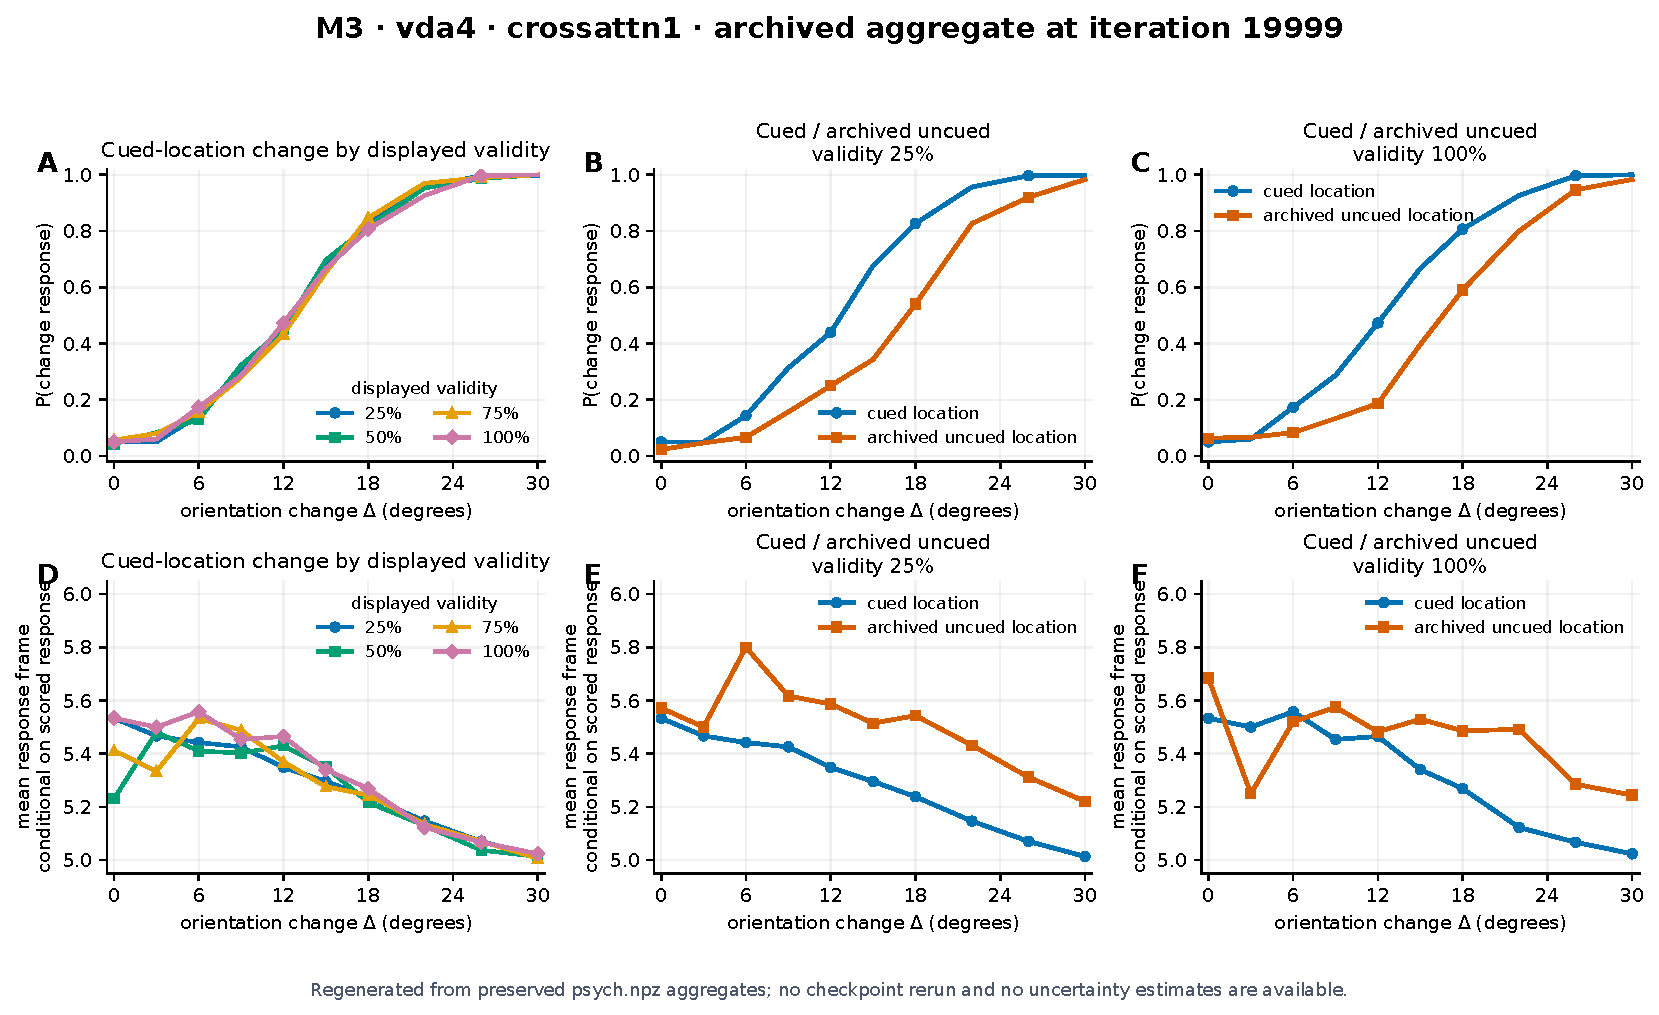
\includegraphics[width=0.89\linewidth]{m3_behavior_vda4_crossattn1.pdf}
\captionof{figure}{\textbf{Historical VDA4, cross-attention.} \eclass{Regenerated from preserved aggregate NPZ; checkpoint not rerun.} Pronounced cued--archived-uncued separation; the uncued index and checkpoint lineage are not cache-proven.}\label{fig:m3-vda4-cross}
\end{center}\end{landscape}

\begin{landscape}\thispagestyle{plain}\begin{center}
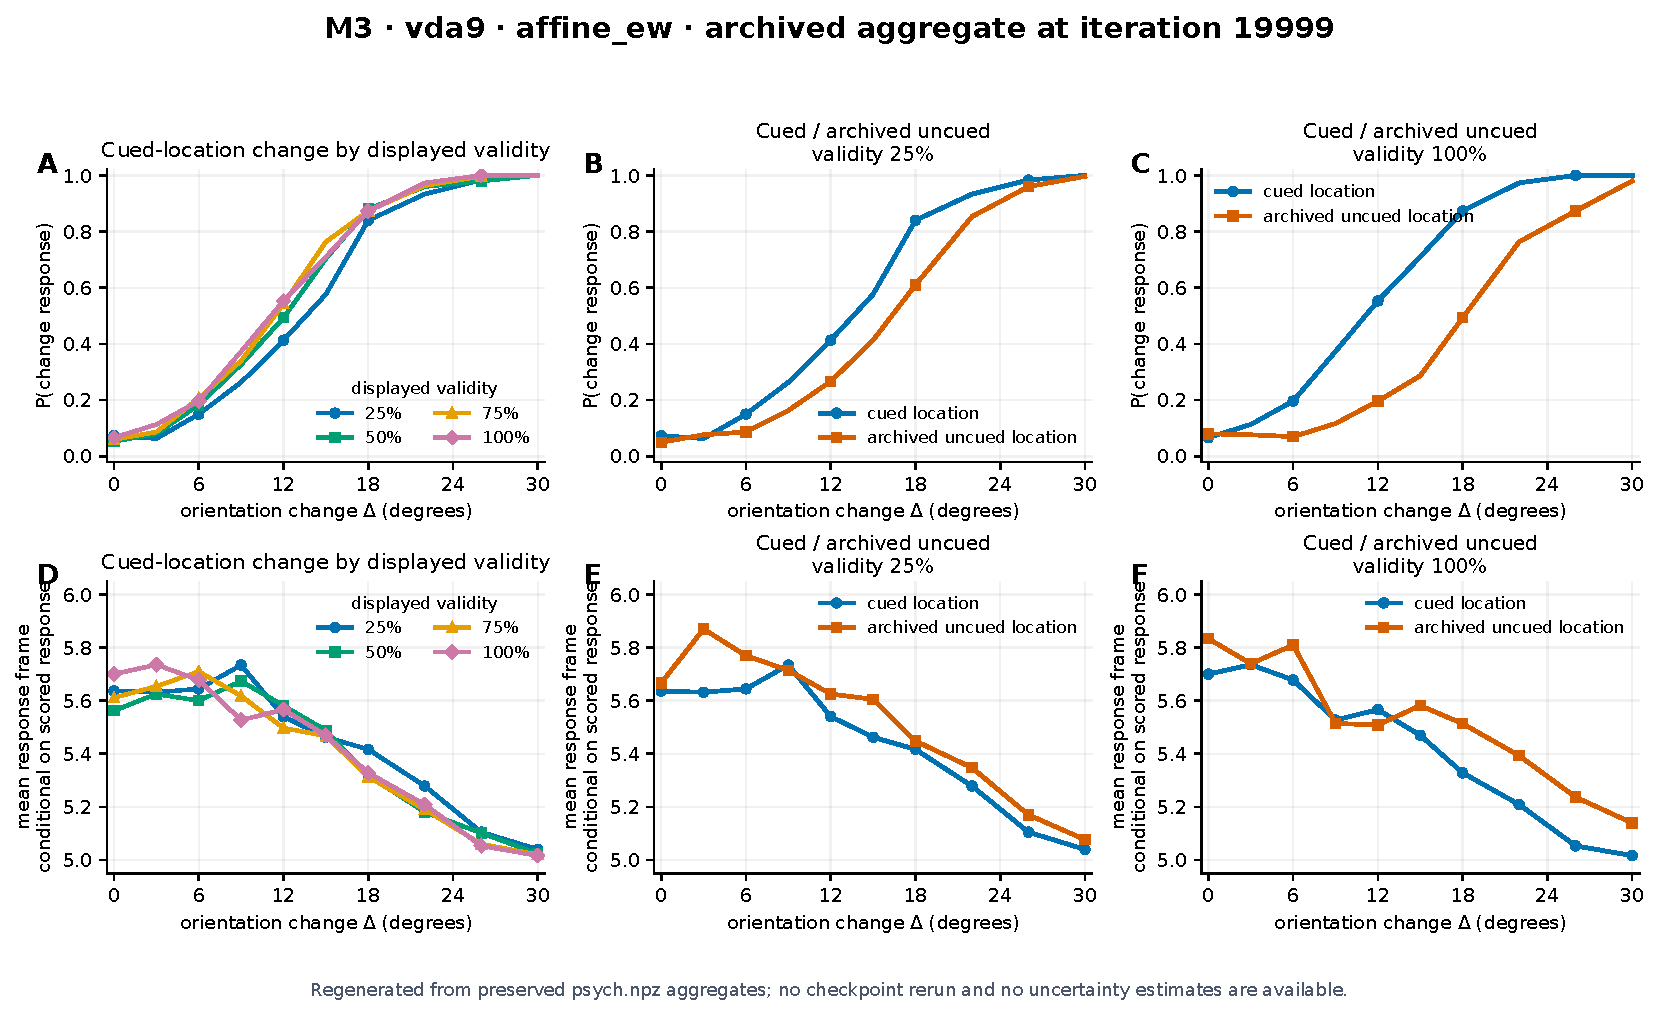
\includegraphics[width=0.89\linewidth]{m3_behavior_vda9_affine_ew.pdf}
\captionof{figure}{\textbf{Historical VDA9, affine feedback.} \eclass{Regenerated from preserved aggregate NPZ; checkpoint not rerun.} Cued and archived uncued point estimates differ; realized cue probability is $p+(1-p)/9$ under natural sampling, though this curve forces location.}\label{fig:m3-vda9-affine}
\end{center}\end{landscape}

\begin{landscape}\thispagestyle{plain}\begin{center}
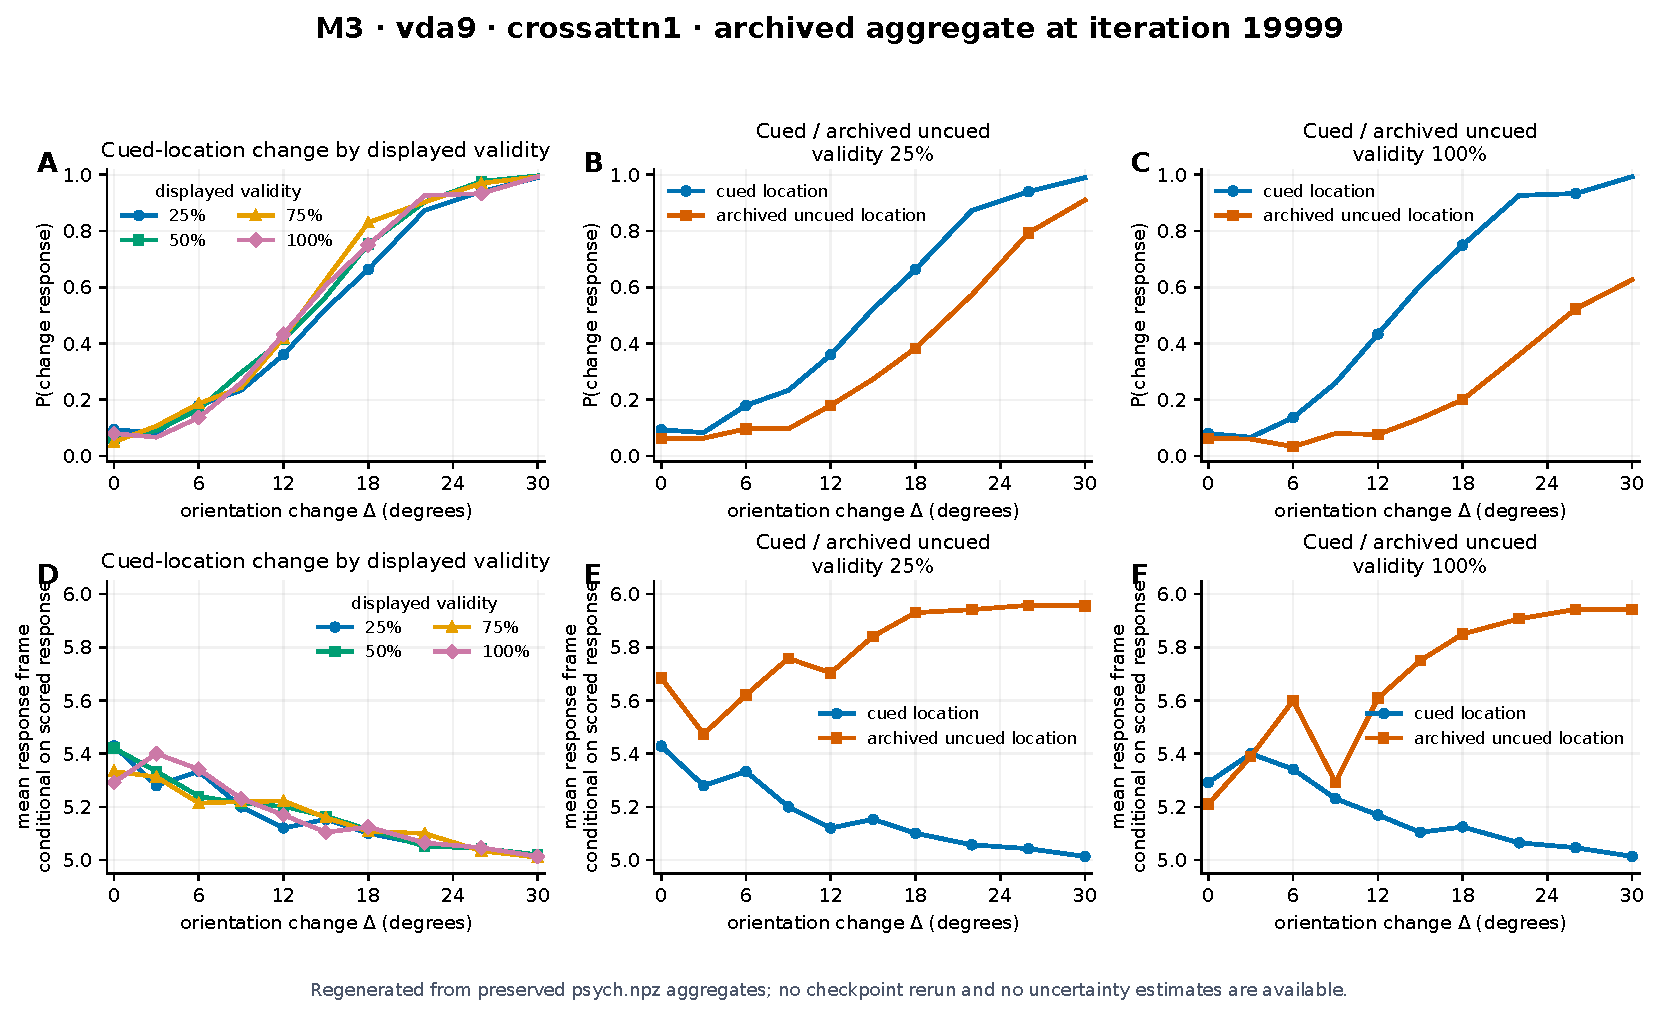
\includegraphics[width=0.89\linewidth]{m3_behavior_vda9_crossattn1.pdf}
\captionof{figure}{\textbf{Historical VDA9, cross-attention.} \eclass{Regenerated from preserved aggregate NPZ; checkpoint not rerun.} Pronounced descriptive cued--archived-uncued separation; geometry, token count, weights, and training differ from smaller tasks, so this is not a controlled capacity estimate.}\label{fig:m3-vda9-cross}
\end{center}\end{landscape}
}

\MThreeFullPlates

\begin{landscape}
\section{Coverage counts by source object}\label{app:coverage-counts}
\begin{center}
\captionof{table}{\textbf{Overall publication-coverage status.} Counts are panel--environment cells, not independent experiments.}\label{tab:coverage-status}
\begin{tabular}{@{}lrr@{}}
\toprule
Status & Cells & Share \\
\midrule
Complete & 118 & 12.4\% \\
Partial & 79 & 8.3\% \\
Available & 149 & 15.7\% \\
Training & 45 & 4.7\% \\
Blocked & 204 & 21.4\% \\
Undefined & 71 & 7.5\% \\
Inapplicable & 286 & 30.0\% \\
\midrule
Total & 952 & 100.0\% \\
\bottomrule
\end{tabular}

\end{center}
\begingroup
\normalsize
\renewcommand{\arraystretch}{1.10}
\begin{longtable}{@{}lrrrrrrrr@{}}
\caption{Coverage counts by source object. Counts are panel--environment cells, not independent experiments. Status codes are C complete, P partial, A available, T training, B blocked, U undefined, and I inapplicable.}\label{tab:object-counts}\\
\toprule
Object & Groups & C & P & A & T & B & U & I \\
\midrule\endfirsthead
\toprule Object & Groups & C & P & A & T & B & U & I \\ \midrule\endhead
M1 & 3 & 40 & 0 & 0 & 0 & 0 & 2 & 0 \\
M2 & 4 & 56 & 0 & 0 & 0 & 0 & 0 & 0 \\
M3 & 6 & 20 & 0 & 0 & 6 & 26 & 8 & 24 \\
M4 & 4 & 2 & 14 & 3 & 4 & 18 & 5 & 10 \\
M5 & 6 & 0 & 24 & 0 & 6 & 26 & 4 & 24 \\
S1 & 1 & 0 & 0 & 14 & 0 & 0 & 0 & 0 \\
S2 & 1 & 0 & 0 & 14 & 0 & 0 & 0 & 0 \\
S3 & 1 & 0 & 0 & 14 & 0 & 0 & 0 & 0 \\
S4 & 1 & 0 & 0 & 14 & 0 & 0 & 0 & 0 \\
S5 & 2 & 0 & 0 & 0 & 0 & 0 & 0 & 28 \\
S6 & 2 & 0 & 0 & 0 & 0 & 0 & 0 & 28 \\
S7 & 2 & 0 & 0 & 0 & 0 & 0 & 0 & 28 \\
S8 & 1 & 0 & 2 & 3 & 1 & 5 & 3 & 0 \\
S9 & 1 & 0 & 2 & 0 & 1 & 8 & 3 & 0 \\
S10 & 1 & 0 & 2 & 5 & 1 & 6 & 0 & 0 \\
S11 & 2 & 0 & 4 & 8 & 2 & 11 & 3 & 0 \\
S12 & 1 & 0 & 2 & 5 & 1 & 6 & 0 & 0 \\
S13 & 5 & 0 & 5 & 27 & 5 & 20 & 13 & 0 \\
S14 & 3 & 0 & 3 & 18 & 3 & 18 & 0 & 0 \\
S15 & 9 & 0 & 9 & 18 & 9 & 36 & 18 & 36 \\
S16 & 6 & 0 & 12 & 6 & 6 & 24 & 12 & 24 \\
S17 & 6 & 0 & 0 & 0 & 0 & 0 & 0 & 84 \\
\bottomrule
\end{longtable}
\endgroup

\end{landscape}

\begin{landscape}
\section{Exact panel--environment disposition matrix}
Environment abbreviations are: Val4 (\env{validity4}); H1/H2/H4/H9/H16 (historical VDA set sizes); Excl (\env{vda\_excl}); PC/PU (cued/uncued probes); and F1/F2/F4/F9/F16 (controlled fixed-grid set sizes). Status codes are C complete, P partial, A available, T training, B blocked, U undefined, and I inapplicable. Empty status groups are shown with an em dash.

\begingroup
\footnotesize
\setlength{\tabcolsep}{2.5pt}
\renewcommand{\arraystretch}{1.08}
\begin{longtable}{@{}p{1.8cm}p{3.9cm}p{2.2cm}p{2.2cm}p{2.0cm}p{2.3cm}p{2.35cm}p{2.5cm}@{}}
\caption{Exact source-panel disposition by environment. The table is generated directly from \texttt{PANEL\_COVERAGE.csv}; comma-separated abbreviations name every environment assigned to each state.}\label{tab:panel-matrix}\\
\toprule
Panel & Purpose & C/P & Available & Training & Blocked & Undefined & Inapplicable \\
\midrule
\endfirsthead
\multicolumn{8}{c}{\tablename\ \thetable\ (continued)}\\
\toprule
Panel & Purpose & C/P & Available & Training & Blocked & Undefined & Inapplicable \\
\midrule
\endhead
\midrule \multicolumn{8}{r}{Continued on next page}\\ \endfoot
\bottomrule \endlastfoot
M1a & trial sequence & C: Val4, H1, H2, H4, H9, H16, Excl, PC, PU, F1, F2, F4, F9, F16 & \textemdash & \textemdash & \textemdash & \textemdash & \textemdash \\
M1b & cue/value configurations & C: Val4, H1, H2, H4, H9, H16, Excl, PC, PU, F1, F2, F4, F9, F16 & \textemdash & \textemdash & \textemdash & \textemdash & \textemdash \\
M1c & cued versus opposing change examples & C: Val4, H2, H4, H9, H16, Excl, PC, PU, F2, F4, F9, F16 & \textemdash & \textemdash & \textemdash & H1, F1 & \textemdash \\
\addlinespace[2pt]
M2a & patching and visual features & C: Val4, H1, H2, H4, H9, H16, Excl, PC, PU, F1, F2, F4, F9, F16 & \textemdash & \textemdash & \textemdash & \textemdash & \textemdash \\
M2b & routing/allocation mechanism & C: Val4, H1, H2, H4, H9, H16, Excl, PC, PU, F1, F2, F4, F9, F16 & \textemdash & \textemdash & \textemdash & \textemdash & \textemdash \\
M2c & recurrent memory update & C: Val4, H1, H2, H4, H9, H16, Excl, PC, PU, F1, F2, F4, F9, F16 & \textemdash & \textemdash & \textemdash & \textemdash & \textemdash \\
M2d & actor/critic temporal loop & C: Val4, H1, H2, H4, H9, H16, Excl, PC, PU, F1, F2, F4, F9, F16 & \textemdash & \textemdash & \textemdash & \textemdash & \textemdash \\
\addlinespace[2pt]
M3A & response rate by cue validity & C: H1, H2, H4, H9 & \textemdash & F16 & H16, F1, F2, F4, F9 & \textemdash & Val4, Excl, PC, PU \\
M3D & conditional logical response frame by displayed validity & C: H1, H2, H4, H9 & \textemdash & F16 & H16, F1, F2, F4, F9 & \textemdash & Val4, Excl, PC, PU \\
M3B & change-response probability: cued versus archived uncued, low displayed validity & C: H2, H4, H9 & \textemdash & F16 & H16, F2, F4, F9 & H1, F1 & Val4, Excl, PC, PU \\
M3C & change-response probability: cued versus archived uncued, high displayed validity & C: H2, H4, H9 & \textemdash & F16 & H16, F2, F4, F9 & H1, F1 & Val4, Excl, PC, PU \\
M3E & conditional logical response frame: cued versus archived uncued, low displayed validity & C: H2, H4, H9 & \textemdash & F16 & H16, F2, F4, F9 & H1, F1 & Val4, Excl, PC, PU \\
M3F & conditional logical response frame: cued versus archived uncued, high displayed validity & C: H2, H4, H9 & \textemdash & F16 & H16, F2, F4, F9 & H1, F1 & Val4, Excl, PC, PU \\
\addlinespace[2pt]
M4A & allocation maps by cue validity and time & P: H1, H2, H4, H9 & \textemdash & F16 & H16, F1, F2, F4, F9 & \textemdash & Val4, Excl, PC, PU \\
M4B & S1 allocation at change time for S1 changes & C: H4, H9; P: H1, H2, Excl & Val4 & F16 & H16, F1, F2, F4, F9 & \textemdash & PC, PU \\
M4C & S1 allocation when another location changes & P: H2, H4, H9 & Val4 & F16 & H16, F2, F4, F9 & H1, Excl, F1 & PC, PU \\
M4D & S1/S4 allocation over trial time & P: H2, H4, H9, Excl & Val4 & F16 & H16, F2, F4, F9 & H1, F1 & PC, PU \\
\addlinespace[2pt]
M5A & response rate: natural/target intervention & P: H1, H2, H4, H9 & \textemdash & F16 & H16, F1, F2, F4, F9 & \textemdash & Val4, Excl, PC, PU \\
M5B & response rate: matched-location intervention contrast & P: H1, H2, H4, H9 & \textemdash & F16 & H16, F2, F4, F9 & F1 & Val4, Excl, PC, PU \\
M5C & response rate: competing-location intervention contrast & P: H1, H2, H4, H9 & \textemdash & F16 & H16, F2, F4, F9 & F1 & Val4, Excl, PC, PU \\
M5D & reaction time: natural/target intervention & P: H1, H2, H4, H9 & \textemdash & F16 & H16, F1, F2, F4, F9 & \textemdash & Val4, Excl, PC, PU \\
M5E & reaction time: matched-location intervention contrast & P: H1, H2, H4, H9 & \textemdash & F16 & H16, F2, F4, F9 & F1 & Val4, Excl, PC, PU \\
M5F & reaction time: competing-location intervention contrast & P: H1, H2, H4, H9 & \textemdash & F16 & H16, F2, F4, F9 & F1 & Val4, Excl, PC, PU \\
\addlinespace[2pt]
S1 & high-level recurrent circuit & \textemdash & Val4, H1, H2, H4, H9, H16, Excl, PC, PU, F1, F2, F4, F9, F16 & \textemdash & \textemdash & \textemdash & \textemdash \\
\addlinespace[2pt]
S2 & patch-wise recurrent memory & \textemdash & Val4, H1, H2, H4, H9, H16, Excl, PC, PU, F1, F2, F4, F9, F16 & \textemdash & \textemdash & \textemdash & \textemdash \\
\addlinespace[2pt]
S3 & immediate-input allocation before memory & \textemdash & Val4, H1, H2, H4, H9, H16, Excl, PC, PU, F1, F2, F4, F9, F16 & \textemdash & \textemdash & \textemdash & \textemdash \\
\addlinespace[2pt]
S4 & memory feedback into allocation & \textemdash & Val4, H1, H2, H4, H9, H16, Excl, PC, PU, F1, F2, F4, F9, F16 & \textemdash & \textemdash & \textemdash & \textemdash \\
\addlinespace[2pt]
S5a & memory-token architecture & \textemdash & \textemdash & \textemdash & \textemdash & \textemdash & Val4, H1, H2, H4, H9, H16, Excl, PC, PU, F1, F2, F4, F9, F16 \\
S5b-e & memory-token behavior/allocation battery & \textemdash & \textemdash & \textemdash & \textemdash & \textemdash & Val4, H1, H2, H4, H9, H16, Excl, PC, PU, F1, F2, F4, F9, F16 \\
\addlinespace[2pt]
S6a & additive Q/K/V architecture & \textemdash & \textemdash & \textemdash & \textemdash & \textemdash & Val4, H1, H2, H4, H9, H16, Excl, PC, PU, F1, F2, F4, F9, F16 \\
S6b-e & additive Q/K/V behavior/allocation battery & \textemdash & \textemdash & \textemdash & \textemdash & \textemdash & Val4, H1, H2, H4, H9, H16, Excl, PC, PU, F1, F2, F4, F9, F16 \\
\addlinespace[2pt]
S7a & multiplicative Q/K/V architecture & \textemdash & \textemdash & \textemdash & \textemdash & \textemdash & Val4, H1, H2, H4, H9, H16, Excl, PC, PU, F1, F2, F4, F9, F16 \\
S7b-e & multiplicative Q/K/V behavior/allocation battery & \textemdash & \textemdash & \textemdash & \textemdash & \textemdash & Val4, H1, H2, H4, H9, H16, Excl, PC, PU, F1, F2, F4, F9, F16 \\
\addlinespace[2pt]
S8-all & all-slot change-location decoding, natural/max allocation, t5/t6 & P: H4, H9 & Val4, PC, PU & F16 & H2, H16, F2, F4, F9 & H1, Excl, F1 & \textemdash \\
\addlinespace[2pt]
S9-all & all-slot location decoding across four allocation conditions & P: H4, H9 & \textemdash & F16 & Val4, H2, H16, PC, PU, F2, F4, F9 & H1, Excl, F1 & \textemdash \\
\addlinespace[2pt]
S10-all & single-slot binary change decoding across allocation conditions & P: H4, H9 & Val4, H1, Excl, PC, PU & F16 & H2, H16, F1, F2, F4, F9 & \textemdash & \textemdash \\
\addlinespace[2pt]
S11-location & actor-layer change-location decoding & P: H4, H9 & Val4, PC, PU & F16 & H2, H16, F2, F4, F9 & H1, Excl, F1 & \textemdash \\
S11-binary & actor-layer binary change decoding & P: H4, H9 & Val4, H1, Excl, PC, PU & F16 & H2, H16, F1, F2, F4, F9 & \textemdash & \textemdash \\
\addlinespace[2pt]
S12-all & graded actor-layer binary decoding under S1 inhibition & P: H4, H9 & Val4, H1, Excl, PC, PU & F16 & H2, H16, F1, F2, F4, F9 & \textemdash & \textemdash \\
\addlinespace[2pt]
S13-all & all-trial Wait/Declare logit scatter and density & P: H9 & Val4, H1, H2, H4, Excl, PC, PU & F16 & H16, F1, F2, F4, F9 & \textemdash & \textemdash \\
S13-S1 & Wait/Declare logit scatter and density for S1 changes & P: H9 & Val4, H1, H2, H4, Excl, PC, PU & F16 & H16, F1, F2, F4, F9 & \textemdash & \textemdash \\
S13-S2 & Wait/Declare logit scatter and density for S2 changes & P: H9 & Val4, H2, H4, PC, PU & F16 & H16, F2, F4, F9 & H1, Excl, F1 & \textemdash \\
S13-S3 & Wait/Declare logit scatter and density for S3 changes & P: H9 & Val4, H4, PC, PU & F16 & H16, F4, F9 & H1, H2, Excl, F1, F2 & \textemdash \\
S13-S4 & Wait/Declare logit scatter and density for S4 changes & P: H9 & Val4, H4, PC, PU & F16 & H16, F4, F9 & H1, H2, Excl, F1, F2 & \textemdash \\
\addlinespace[2pt]
S14-natural & natural S1-change logit scatter/density & P: H9 & Val4, H1, H4, Excl, PC, PU & F16 & H2, H16, F1, F2, F4, F9 & \textemdash & \textemdash \\
S14-max & maximal S1 allocation logit scatter/density & P: H9 & Val4, H1, H4, Excl, PC, PU & F16 & H2, H16, F1, F2, F4, F9 & \textemdash & \textemdash \\
S14-zero & zero S1 allocation logit scatter/density & P: H9 & Val4, H1, H4, Excl, PC, PU & F16 & H2, H16, F1, F2, F4, F9 & \textemdash & \textemdash \\
\addlinespace[2pt]
S15A & TD error by cue/change location & P: H9 & H2, H4 & F16 & H16, F2, F4, F9 & H1, F1 & Val4, Excl, PC, PU \\
S15B & TD error with target allocation clamp, low cue & P: H9 & H2, H4 & F16 & H16, F2, F4, F9 & H1, F1 & Val4, Excl, PC, PU \\
S15C & TD error with target allocation clamp, high cue & P: H9 & H2, H4 & F16 & H16, F2, F4, F9 & H1, F1 & Val4, Excl, PC, PU \\
S15D & TD error by allocation dose and location & P: H9 & H2, H4 & F16 & H16, F2, F4, F9 & H1, F1 & Val4, Excl, PC, PU \\
S15E & TD error under competing-location clamp, low cue & P: H9 & H2, H4 & F16 & H16, F2, F4, F9 & H1, F1 & Val4, Excl, PC, PU \\
S15F & TD error under competing-location clamp, high cue & P: H9 & H2, H4 & F16 & H16, F2, F4, F9 & H1, F1 & Val4, Excl, PC, PU \\
S15G & value by change magnitude with target clamp & P: H9 & H2, H4 & F16 & H16, F2, F4, F9 & H1, F1 & Val4, Excl, PC, PU \\
S15H & value by opposing-location allocation dose & P: H9 & H2, H4 & F16 & H16, F2, F4, F9 & H1, F1 & Val4, Excl, PC, PU \\
S15I & hit rate by opposing-location allocation dose & P: H9 & H2, H4 & F16 & H16, F2, F4, F9 & H1, F1 & Val4, Excl, PC, PU \\
\addlinespace[2pt]
S16A & criterion vs allocation at change & P: H4, H9 & H2 & F16 & H16, F2, F4, F9 & H1, F1 & Val4, Excl, PC, PU \\
S16B & criterion vs cue-time allocation with change-time control & P: H4, H9 & H2 & F16 & H16, F2, F4, F9 & H1, F1 & Val4, Excl, PC, PU \\
S16C & criterion vs cue-time allocation & P: H4, H9 & H2 & F16 & H16, F2, F4, F9 & H1, F1 & Val4, Excl, PC, PU \\
S16D & sensitivity vs allocation at change & P: H4, H9 & H2 & F16 & H16, F2, F4, F9 & H1, F1 & Val4, Excl, PC, PU \\
S16E & sensitivity vs cue-time allocation with change-time control & P: H4, H9 & H2 & F16 & H16, F2, F4, F9 & H1, F1 & Val4, Excl, PC, PU \\
S16F & sensitivity vs cue-time allocation & P: H4, H9 & H2 & F16 & H16, F2, F4, F9 & H1, F1 & Val4, Excl, PC, PU \\
\addlinespace[2pt]
S17-action-behavior & three behavioral rows: supervised actions & \textemdash & \textemdash & \textemdash & \textemdash & \textemdash & Val4, H1, H2, H4, H9, H16, Excl, PC, PU, F1, F2, F4, F9, F16 \\
S17-belief-behavior & three behavioral rows: supervised beliefs & \textemdash & \textemdash & \textemdash & \textemdash & \textemdash & Val4, H1, H2, H4, H9, H16, Excl, PC, PU, F1, F2, F4, F9, F16 \\
S17-rl-behavior & three behavioral rows: reinforcement learning & \textemdash & \textemdash & \textemdash & \textemdash & \textemdash & Val4, H1, H2, H4, H9, H16, Excl, PC, PU, F1, F2, F4, F9, F16 \\
S17-action-allocation & allocation row: supervised actions & \textemdash & \textemdash & \textemdash & \textemdash & \textemdash & Val4, H1, H2, H4, H9, H16, Excl, PC, PU, F1, F2, F4, F9, F16 \\
S17-belief-allocation & allocation row: supervised beliefs & \textemdash & \textemdash & \textemdash & \textemdash & \textemdash & Val4, H1, H2, H4, H9, H16, Excl, PC, PU, F1, F2, F4, F9, F16 \\
S17-rl-allocation & allocation row: reinforcement learning & \textemdash & \textemdash & \textemdash & \textemdash & \textemdash & Val4, H1, H2, H4, H9, H16, Excl, PC, PU, F1, F2, F4, F9, F16 \\
\end{longtable}
\endgroup

\end{landscape}

\begin{landscape}
\section{Matched-width constituent values}\label{app:matched-width-constituents}
The tables expose the absolute and within-checkpoint values behind the d256-minus-d128 summary in Section~\ref{sec:width-behavior}. They are regenerated by \path{reports/vda_series/manuscript/build_constituent_tables.py}, which verifies all twelve shard hashes against the immutable upstream manifest before reading arrays; the machine-readable companion is \path{generated/matched_width_constituents.json}.
\begingroup\scriptsize\setlength{\tabcolsep}{2.7pt}
\captionof{table}{\textbf{Absolute valid-location response probabilities.} Checkpoint-recomputed values at displayed validity 0.75; each cell uses 300 trials. These are the constituents behind Figure~\ref{fig:matched-width}A, not replicated estimates of a width effect.}\label{tab:absolute-behavior}
\begin{center}
\begin{tabular}{@{}llr*{10}{r}@{}}
\toprule
Task & Routing & Width & \multicolumn{10}{c}{Orientation change (degrees)} \\
\cmidrule(lr){4-13}
 & & & 2 & 6 & 10 & 14 & 18 & 22 & 26 & 30 & 34 & 38 \\ 
\midrule
VDA1 & \texttt{affine} & 128 & 0.133 & 0.250 & 0.460 & 0.697 & 0.903 & 0.923 & 0.960 & 0.957 & 0.953 & 0.947 \\
VDA1 & \texttt{affine} & 256 & 0.123 & 0.230 & 0.487 & 0.653 & 0.907 & 0.917 & 0.953 & 0.953 & 0.947 & 0.963 \\
VDA1 & \texttt{cross-attn} & 128 & 0.060 & 0.123 & 0.313 & 0.520 & 0.717 & 0.843 & 0.863 & 0.873 & 0.890 & 0.857 \\
VDA1 & \texttt{cross-attn} & 256 & 0.177 & 0.287 & 0.480 & 0.730 & 0.810 & 0.910 & 0.897 & 0.907 & 0.923 & 0.897 \\
VDA4 & \texttt{affine} & 128 & 0.093 & 0.177 & 0.437 & 0.663 & 0.833 & 0.947 & 0.973 & 0.997 & 1.000 & 1.000 \\
VDA4 & \texttt{affine} & 256 & 0.120 & 0.337 & 0.587 & 0.777 & 0.933 & 0.980 & 0.990 & 0.997 & 0.997 & 1.000 \\
VDA4 & \texttt{cross-attn} & 128 & 0.063 & 0.140 & 0.410 & 0.617 & 0.803 & 0.967 & 0.980 & 1.000 & 1.000 & 1.000 \\
VDA4 & \texttt{cross-attn} & 256 & 0.037 & 0.113 & 0.303 & 0.487 & 0.690 & 0.923 & 0.953 & 0.993 & 1.000 & 1.000 \\
VDA9 & \texttt{affine} & 128 & 0.073 & 0.170 & 0.420 & 0.640 & 0.863 & 0.970 & 0.990 & 1.000 & 1.000 & 1.000 \\
VDA9 & \texttt{affine} & 256 & 0.087 & 0.140 & 0.407 & 0.597 & 0.813 & 0.963 & 0.983 & 0.997 & 1.000 & 1.000 \\
\bottomrule
\end{tabular}
\end{center}
\endgroup

\begingroup\scriptsize\setlength{\tabcolsep}{4.0pt}
\captionof{table}{\textbf{Within-checkpoint clamp constituents.} Each entry is $D_{w,x}(b)=d'_{w,x}(b)-d'_{w,x}(0)$ from 250 trials per bias, condition, and checkpoint. VDA1 invalid-location effects are undefined and therefore absent. Figure~\ref{fig:matched-width}C--D plots $W_x(b)=D_{256,x}(b)-D_{128,x}(b)$.}\label{tab:clamp-constituents}
\begin{center}
\begin{tabular}{@{}llll*{5}{r}@{}}
\toprule
Task & Routing & Condition & Width & \multicolumn{5}{c}{Assigned key-logit bias $b$} \\
\cmidrule(lr){5-9}
 & & & & -6 & -3 & 0 & 3 & 6 \\ 
\midrule
VDA1 & \texttt{affine} & valid & 128 & -1.681 & -1.124 & 0.000 & -0.474 & -0.572 \\
VDA1 & \texttt{affine} & valid & 256 & -0.017 & -0.017 & 0.000 & -0.017 & -0.020 \\
VDA1 & \texttt{cross-attn} & valid & 128 & -0.470 & 0.054 & 0.000 & 0.071 & 0.137 \\
VDA1 & \texttt{cross-attn} & valid & 256 & 0.087 & 0.028 & 0.000 & -0.019 & -0.102 \\
VDA4 & \texttt{affine} & valid & 128 & -1.384 & -0.622 & 0.000 & 0.247 & 0.092 \\
VDA4 & \texttt{affine} & invalid & 128 & 0.375 & 0.351 & 0.000 & -0.785 & -1.484 \\
VDA4 & \texttt{affine} & valid & 256 & -0.491 & -0.176 & 0.000 & 0.046 & -0.156 \\
VDA4 & \texttt{affine} & invalid & 256 & 0.284 & 0.146 & 0.000 & -0.377 & -0.787 \\
VDA4 & \texttt{cross-attn} & valid & 128 & -0.544 & -0.426 & 0.000 & -0.297 & -0.456 \\
VDA4 & \texttt{cross-attn} & invalid & 128 & 0.172 & 0.172 & 0.000 & -0.610 & -0.750 \\
VDA4 & \texttt{cross-attn} & valid & 256 & -0.736 & -0.577 & 0.000 & -0.009 & -0.047 \\
VDA4 & \texttt{cross-attn} & invalid & 256 & 0.117 & 0.133 & 0.000 & -0.434 & -0.574 \\
VDA9 & \texttt{affine} & valid & 128 & -0.978 & -0.300 & 0.000 & -0.097 & -0.199 \\
VDA9 & \texttt{affine} & invalid & 128 & 0.420 & 0.391 & 0.000 & -0.187 & -0.462 \\
VDA9 & \texttt{affine} & valid & 256 & -0.046 & 0.040 & 0.000 & 0.086 & 0.097 \\
VDA9 & \texttt{affine} & invalid & 256 & 0.150 & 0.076 & 0.000 & -0.160 & -0.378 \\
\bottomrule
\end{tabular}
\end{center}
\endgroup

\end{landscape}

\section{Artifact locations and provenance classes}
\begingroup
\small
\begin{tabularx}{\textwidth}{@{}p{3.2cm}Y Y@{}}
\toprule
Artifact & Path & Provenance class\\
\midrule
This manuscript & \path{reports/vda_series/manuscript/VDA_Set_Size.pdf} & Restructured narrative manuscript, updated 20 July 2026\\
M1 task products & \path{reports/vda_series/figures/task/} & Newly regenerated deterministic specifications\\
M2 architecture & \path{reports/vda_series/figures/architecture/} & Newly authored source-derived specification diagrams\\
M3 behavior & \path{reports/vda_series/figures/behavior/} & Newly regenerated plots from preserved aggregate NPZ\\
First-wave checkpoint products & \path{reports/vda_series/figures/first_wave/} & Byte-identical publication snapshots from the independently approved 96/300 production build\\
First-wave production QA & \path{RViT_plus_paper_jepa_grid9/reports/vda_series/first_wave_20260711_production_QA.md} & Dated semantic, provenance, format, and visual approval record\\
Matched-width publication snapshots & \path{reports/vda_series/figures/matched_width/} & Locally manifested PDF/SVG/PNG/JSON and production-manifest projection from the audited v15 summary\\
Matched-width production root & \path{reports/vda_series/matched_width_20260712_production_v15/} & Exact-inventory summary bound to the immutable 12-file upstream battery\\
VDA16 cross-attention production shard & \path{RViT_plus_paper_jepa_grid9/reports/vda_series/vda16_crossattn_nodecay_20260719_production/} & Terminal checkpoint-bound, validation-gated controlled fixed-grid evidence\\
VDA16 affine production shard & \path{RViT_plus_paper_jepa_grid9/reports/vda_series/vda16_affine_nodecay_20260720_production/} & Terminal checkpoint-bound, validation-gated controlled fixed-grid evidence; freezes the admitted cross-attention companion shard for paired context\\
VDA16 paired-location attention experiment & \path{RViT_plus_paper_jepa_grid9/reports/vda_series/vda16_cued_vs_opposite_attention_20260719/} & Checkpoint-rerun trial cache, behavior/attention curves, spatial maps, source snapshot, and hash manifest\\
Logistic psychometric-fit re-analysis & \path{reports/vda_series/figures/psychometric_fits/} & New re-analysis of already-cached first-wave/VDA16 arrays; no checkpoint access\\
Change-location intervention (VDA16) & \path{RViT_plus_paper_jepa_grid9/reports/vda_series/change_location_intervention_20260719/} & Checkpoint-recomputed paired intervention; VDA4/VDA9 cells recorded blocked (missing checkpoint files)\\
Memory-decay architecture comparison & \path{RViT_plus_paper_jepa_grid9/analysis/vda4_decay_comparison.py}, \path{vda4_crossattn_decay_series.py} & Checkpoint-recomputed, paired frozen-checkpoint comparison\\
Panel inventory & \path{reports/vda_series/MAH_SOURCE_PANEL_INVENTORY.md} & Newly authored source-grounded inventory\\
Coverage matrix & \path{reports/vda_series/PANEL_COVERAGE.csv} & Newly authored machine-readable disposition matrix\\
Older upgraded manuscript & \path{reports/upgraded_paper/manuscript/main.pdf} & Rebuilt from an older manuscript lineage; not this report\\
Preserved VDA9 reports & historical report directories & Preserved older artifacts; visually audited, not relabeled as new\\
\bottomrule
\end{tabularx}
\endgroup

\clearpage
\begin{thebibliography}{9}
\bibitem{mah2025} J. Morgan, L. Albanna, and J. P. Herman. \emph{Recurrent vision transformers model visual attention through feedback}. arXiv:2502.10955v1, 2025.

\bibitem{carrasco2011} M. Carrasco. Visual attention: the past 25 years. \emph{Vision Research}, 2011. doi:10.1016/j.visres.2011.04.012.

\bibitem{herman2017} J. P. Herman and R. J. Krauzlis. Color-change detection activity in the primate superior colliculus. \emph{eNeuro}, 2017. doi:10.1523/ENEURO.0046-17.2017.

\bibitem{luo2018} T. Z. Luo and J. H. R. Maunsell. Attentional changes in either criterion or sensitivity are associated with robust modulations in lateral prefrontal cortex. \emph{Neuron}, 2018. doi:10.1016/j.neuron.2018.02.007.

\bibitem{moore2003} T. Moore and K. M. Armstrong. Selective gating of visual signals by microstimulation of frontal cortex. \emph{Nature}, 2003. doi:10.1038/nature01341.

\bibitem{cavanaugh2004} J. Cavanaugh and R. H. Wurtz. Subcortical modulation of attention counters change blindness. \emph{Journal of Neuroscience}, 2004. doi:10.1523/JNEUROSCI.3724-04.2004.

\bibitem{luck1997} S. J. Luck and E. K. Vogel. The capacity of visual working memory for features and conjunctions. \emph{Nature}, 1997. doi:10.1038/36846.

\bibitem{awh2001} E. Awh and J. Jonides. Overlapping mechanisms of attention and spatial working memory. \emph{Trends in Cognitive Sciences}, 2001. doi:10.1016/S1364-6613(00)01593-X.

\bibitem{panichello2021} M. F. Panichello and T. J. Buschman. Shared mechanisms underlie the control of working memory and attention. \emph{Nature}, 2021. doi:10.1038/s41586-021-03390-w.
\end{thebibliography}

\end{document}
